\chapter[Reconstrução da Física do Canal eGamma do Experimento ATLAS]
{Reconstrução da Física do Canal e/$\gamma$ do Experimento ATLAS}
\label{cap:reco}

\newacronym[type=Abrev]{t2calo}{\emph{T2Calo}}{Algoritmo para a Reconstrução do
Calorímetro no Segundo Nível de Filtragem} 
\newacronym[type=Abrev]{hltringer}{\emph{HLT\_Ringer}}{HLT\_EgammaCaloRinger} 
\glsunset{t2calo}

A alta energia e luminosidade do \gls{lhc} (Seção~\ref{sec:lhc}) oferecem um alto alcance para
explorar física, desde a medição precisa de propriedades de objetos conhecidos, a
ultrapassar a fronteira de energias onde a física ainda não havia sido experimentada.
Por ser um detector de propósito geral, o \gls{atlas} (Seção~\ref{sec:ATLAS}) deve ser capaz de
explorar diversos dos objetivos do \gls{lhc} (Subseção~\ref{ssec:obj_lhc}), e
para isso ele precisar ter a capacidade de explorar um largo espectro de assinaturas
físicas. Esse fato guiou a otimização do projeto do \gls{atlas}, dando as especificações de sensibilidade e precisão do
detector para que seja possível através das assinaturas realizar a reconstrução
com precisão da física ocorrida nas colisões. O foco principal é na busca pelo
bóssom de Higgs \cite{ATLAS_TDR2}, com o objetivo de provar a origem da escala
eletrofraca\footnote{A escala eletrofraca existe somente no estado primitivo descrito na
Subseção~\ref{ssec:bossoms}.}. 

A física se apoia em algoritmos
para realizar a busca pelas assinaturas, sendo este capítulo dedicado aos
algoritmos que fazem a reconstrução do Canal \gls{eg},
onde se deseja encontrar as assinaturas dessas partículas (e dos pósitrons, que
tem a mesma assinatura de elétrons, excluindo a direção de deflexão de seus
traços, oposta àquela de elétrons devido a sua carga positiva). A identificação
dessas partículas é de fundamental importância por formarem os canais de
decaimentos mais limpos do bóssom de Higgs (Sessão~\ref{sec:busca_higgs}). Além
disso, outras partículas como o bóssom Z e partícula $\text{J}/\Psi$, podem ser
utilizadas para melhorar a escala de medida de energia dos calorímetros e
estudar sua linearidade de resposta por terem suas massas bem conhecidas, 
em especial os decaimentos de elétrons do
$\text{J}/\Psi$ para baixas energias ($\gls{Et} > 5$ GeV), onde se esperam encontrar 
decaimentos leptônicos do bóssom de Higgs de menor energia ($\gls{Et} > 7$ GeV).
Outras assinaturas experimentais são as de hádrons e jatos, que serão tratadas
quando abordando o Canal \gls{eg}, por serem o ruído de fundo do qual se deseja
filtrar nesse canal. Entretanto existem setores de física que se
interessam por esses decaimentos, como o já citado decaimento do bóssom W em jatos
duplos\footnote{A citação foi realizada no Subtópico~\ref{par:cal_part_id}.}. 
Além disso, múons constituem de outras assinaturas, uma vez que interagem
pouco com os calorímetros, tendo seu próprio subsistema, o Espectômetro de
Múons. Existem outras três assinaturas:
táons, sabores pesados e léptons neutrinos. Os táons decaem
rapidamente em múons (ou elétrons) e mais dois neutrinos, ou ainda, em um ou três
píons carregados, de forma que sua assinatura é
feita nos espectometros de múons (ou calorímetro), ou de chuveiros \gls{had} com um ou três
traços isolados apontando para o chuveiro. Os sabores pesados procuram
assinaturas de mésons pesados, que geralmente decaem a menos de 1 mm do ponto de
colisão, sendo necessário criar um vértice secundário que será identificado com
a alta precisão do Detector de Pixel. Finalmente, léptons neutrinos escapam da
detecção, para sua assinatura é utilizada a propriedade de conservação de
\gls{pt}, de modo que, quando há quantidade suficiente de \gls{ptmiss}, há indicios
de que algo escapou do processo de detecção.

Os algoritmos são implementados em dois ambientes diferentes, um ambiente mais
restrito, necessário devido ao alto nível de ruído físico gerado nas condições 
impostas do \gls{lhc} (citadas no Tópico~\ref{sssec:minb_ue_pileup}): o
\glsdesc{sf} (Seção~\ref{sec:sf}). Nesse ambiente o tempo de discriminação 
é limitado a latência suportada pela capacidade computacional das máquinas localizadas 
no \gls{ip}1. O trabalho segue com o desenvolvimento do algoritmo
\acrlong{hltringer} (Subseção~\ref{ssec:hlt_ringer}), um algoritmo alternativo proposto para o
Segundo Nível de Filtragem desse sistema. A versão implementada pela
colaboração, o \gls{t2calo} (Subseção~\ref{ssec:cadeia_egamma}), 
também é descrita em detalhes. Por sua vez o outro ambiente, o \glsdesc{sr}
(Seção~\ref{sec:sr}), visa fazer uma análise mais precisa dos eventos de colisão e da 
física gerada, sendo o \glsdesc{sf}, nos níveis mais altos de filtragem, 
nada mais que uma versão restringida baseada no mesmo. Para que a Colaboração tenha 
um melhor contato com o algoritmo proposto e entenda o seu funcionamento, se fez
necessário a implementação (Tópico~\ref{sssec:egringer_impl}) de uma versão no Sistema 
de \glsdesc{sr} (Subseção~\ref{ssec:egringer}) para que os físicos o utilizassem nas suas 
análises a posteriori. A versão padrão (Subseção~\ref{ssec:egamma}) utilizada
pelos físicos também foi abordada.

\section{Busca pelo bóssom de Higgs}
\label{sec:busca_higgs}

\newacronym[type=Simb]{mh}{\ensuremath{m_H}}{massa do bóssom de Higgs} 
\newacronym[type=Abrev]{lep}{LEP}{\emph{Large Electron Positron Collider}} 
\glsunset{mh}

O bóssom de Higgs no setor do \gls{mp} é amplamente irrestrito, de forma que sua
massa, \acrshort{mh}, não é prevista pela teoria. Um limite superior na ordem de
$\sim$1 TeV teórico, e um limite inferior experimental\footnote{As exclusões
citadas foram feitas para um nível de confiança de 95\%.\label{fn:95cl}} de 95,2
GeV \cite{lep_higgs_1999} por um experimento anterior do \gls{cern}, o \gls{lep}, determinam a região para a qual
se esperava encontrar o bóssom de Higgs durante a época das últimas propostas técnicas
do projeto do \gls{atlas} \cite{ATLAS_TDR,ATLAS_TDR2}, por volta de 1999. 

Um estudo do potêncial de descoberta do bóssom de Higgs através de seus
possíveis canais de decaimentos explorados pelo programa de física do
\gls{atlas} foi revisado na propostas citadas. Esses canais são:

\begin{itemize}
\item $H\rightarrow\gamma\gamma$ (110 a 150 GeV/$c^2$), produção direta;
\item $H\rightarrow\gamma\gamma$ (110 a 150 GeV/$c^2$), da produção associada $WH$, $ZH$ e
$t\bar{t}H$, usando um lépton (e, $\mu$) rotulado do decaimento dos bóssom W, Z ou
do quark \emph{top};
\item $H\rightarrow b\bar{b}$ (110 a 130 GeV/$c^2$), da produção associada $WH$, $ZH$ e
$t\bar{t}H$, usando um lépton (e, $\mu$) rotulado do decaimento dos bóssom W, Z ou
do quark \emph{top};
\item $H\rightarrow ZZ^*\rightarrow4l$ (110 a 600 GeV/$c^2$. O símbolo $^*$ representa uma partícula 
que está fora de sua fronteira de massa\footnote {Na literatura em inglês 
\emph{off the mass shell}, ou simplesmente \emph{off
shell}.} na relação massa-momento dada pela equação~\ref{eq:rel_mom}. Essas
partículas só existem como estados intermediários, constituindo partículas
virtuais, e estão de acordo com o princípio da incerteza, em que as partículas
só podem existir nesse estado durante um tempo menor que uma fração da
constante 
de Plank pela diferença de energia, ou $\Delta E \Delta t \gtrsim h$), onde l
representa estes léptons: $e,\mu$; 
\item $H\rightarrow ZZ\rightarrow4l$ e $H\rightarrow ZZ\rightarrow ll\nu\nu$i
(200 a 600 GeV/$c^2$), aqui $\nu$ são os léptons neutrinos;
\item $H\rightarrow WW\rightarrow l\nu jj$ e $H\rightarrow ZZ\rightarrow ll jj$
($\sim$600 a 1 TeV),
onde $jj$ representa o decaimento em jatos duplos;
\item $H\rightarrow WW^*\rightarrow l\nu l\nu$ (110 a 300 GeV/$c^2$). 
\end{itemize}


Nesse estudo se utilizou simulações
de \gls{mc} do \emph{Pythia}, através da significância desses 
canais numa região de 80-1000 GeV/$c^2$ (lembrando que na época só havia sido excluído
o bóssom de Higgs para \gls{mh} < 95,2), utilizando os valores de resposta dos
subdectores, resolução e capacidade esperadas de identificação de sinais e rejeição 
de ruídos redutivéis. 
Os resultados desse estudo estão resumidos na Figura~\ref{fig:higgs_sim_atlas},
mostrando a significância do sinal para uma luminosidade integrada\footnote{A 
luminosidade integrada, como seu nome indica, não passa da integral da luminosidade 
instantânea no tempo de operação do \gls{lhc}: $\int{L_{inst} dt}$.} de
100 $\text{fb}^{-1}$. Para efeito de comparação na
Figura~\ref{fig:higgs_branch_ratio} há as relações entre os canais
e seus alcânces em massa. A Figura~\ref{fig:higgs_production} contêm a seção
de choque esperada para as possíveis massas.

\begin{figure}[ht!]
    \label{fig:higgs_expected}
    \begin{center}
%
        \subfigure[]{%
            \label{fig:higgs_branch_ratio}
            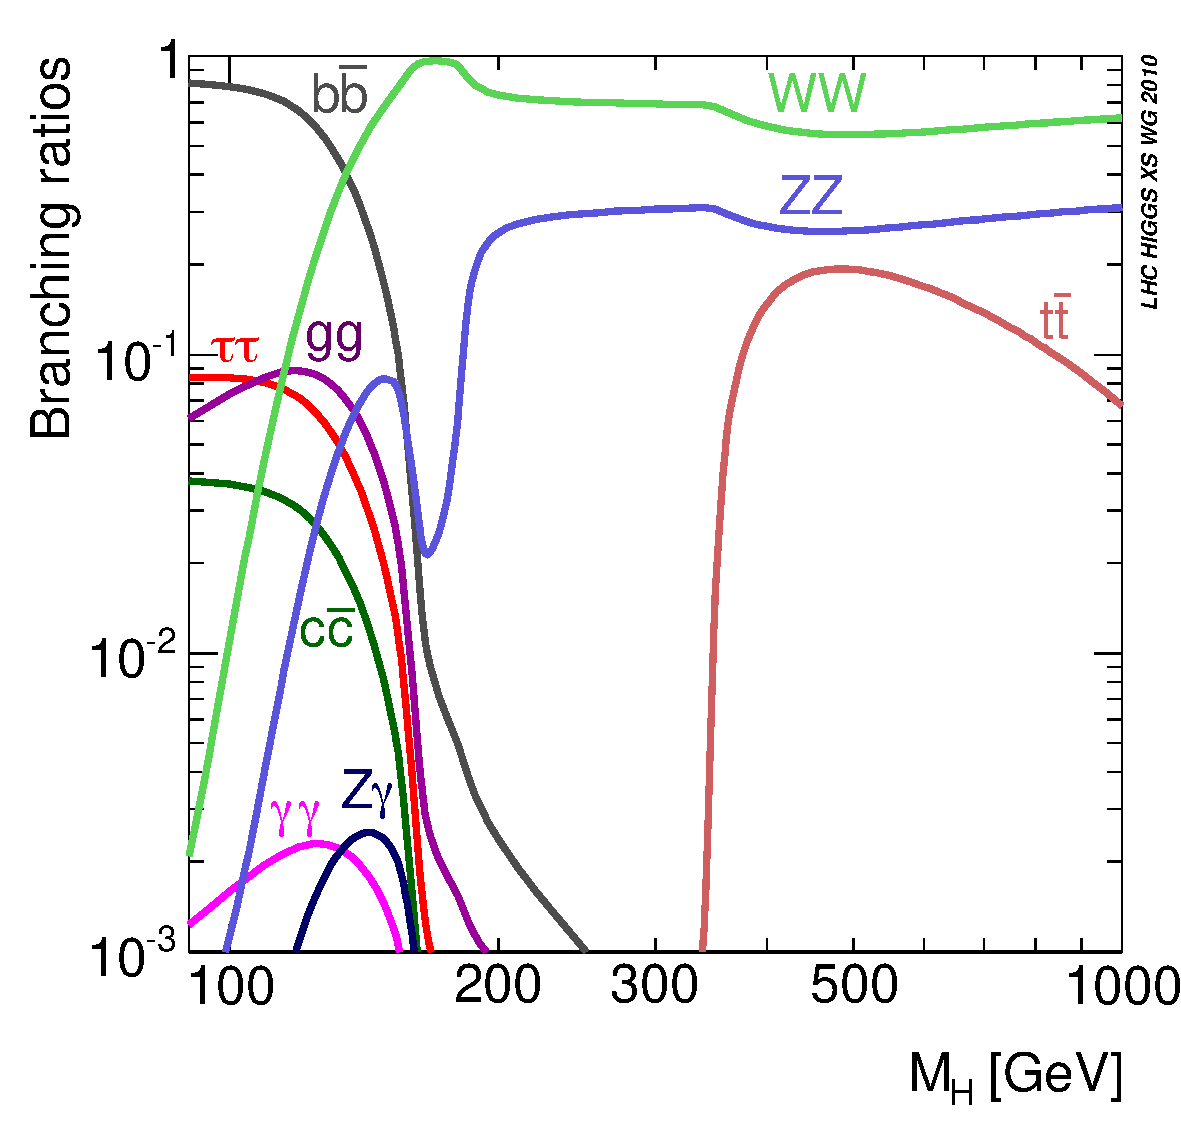
\includegraphics[width=0.47\textwidth,height=6cm]{imagens/higgs_branch_ratio.pdf}
        }%\hspace{0.1\textwidth}
        \subfigure[]{
            \label{fig:higgs_production}
            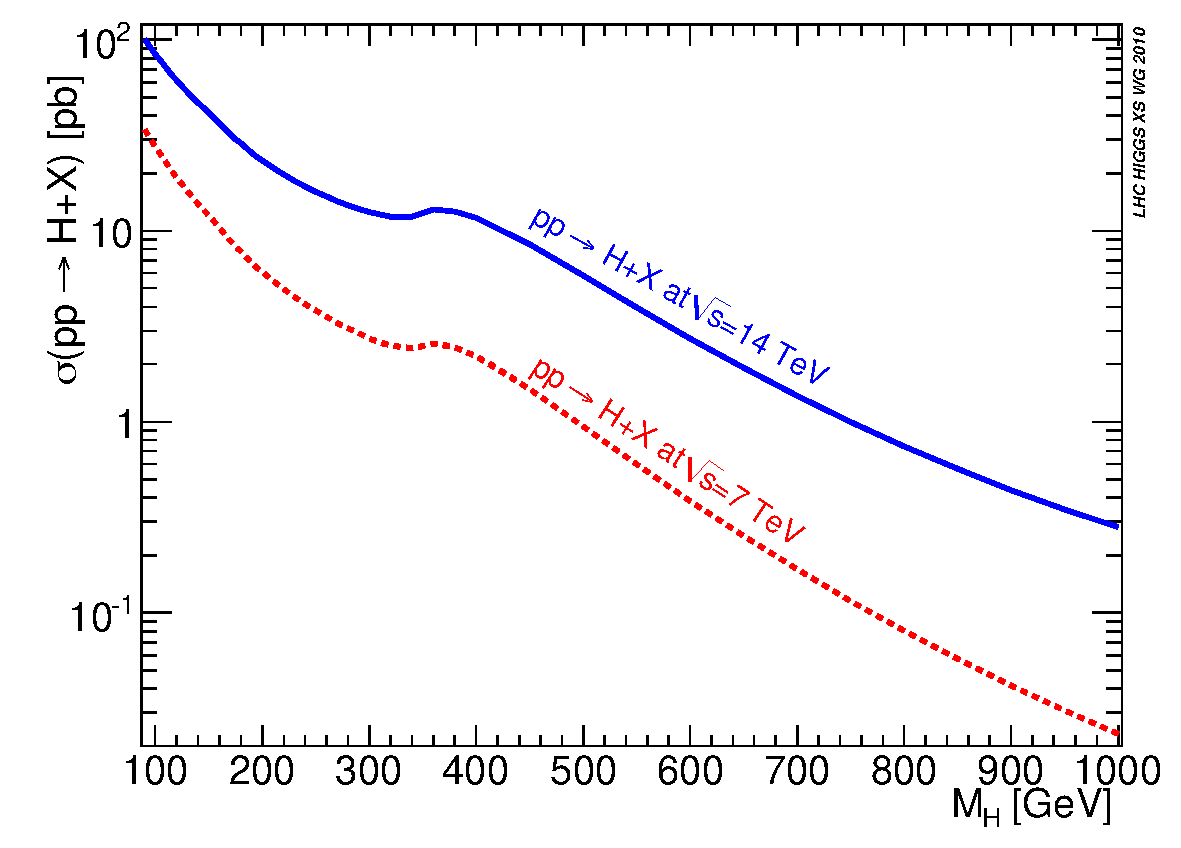
\includegraphics[width=0.47\textwidth,height=6cm]{imagens/higgs_production.pdf}
        }\\
        \subfigure[]{%
            \label{fig:higgs_sim_atlas}
            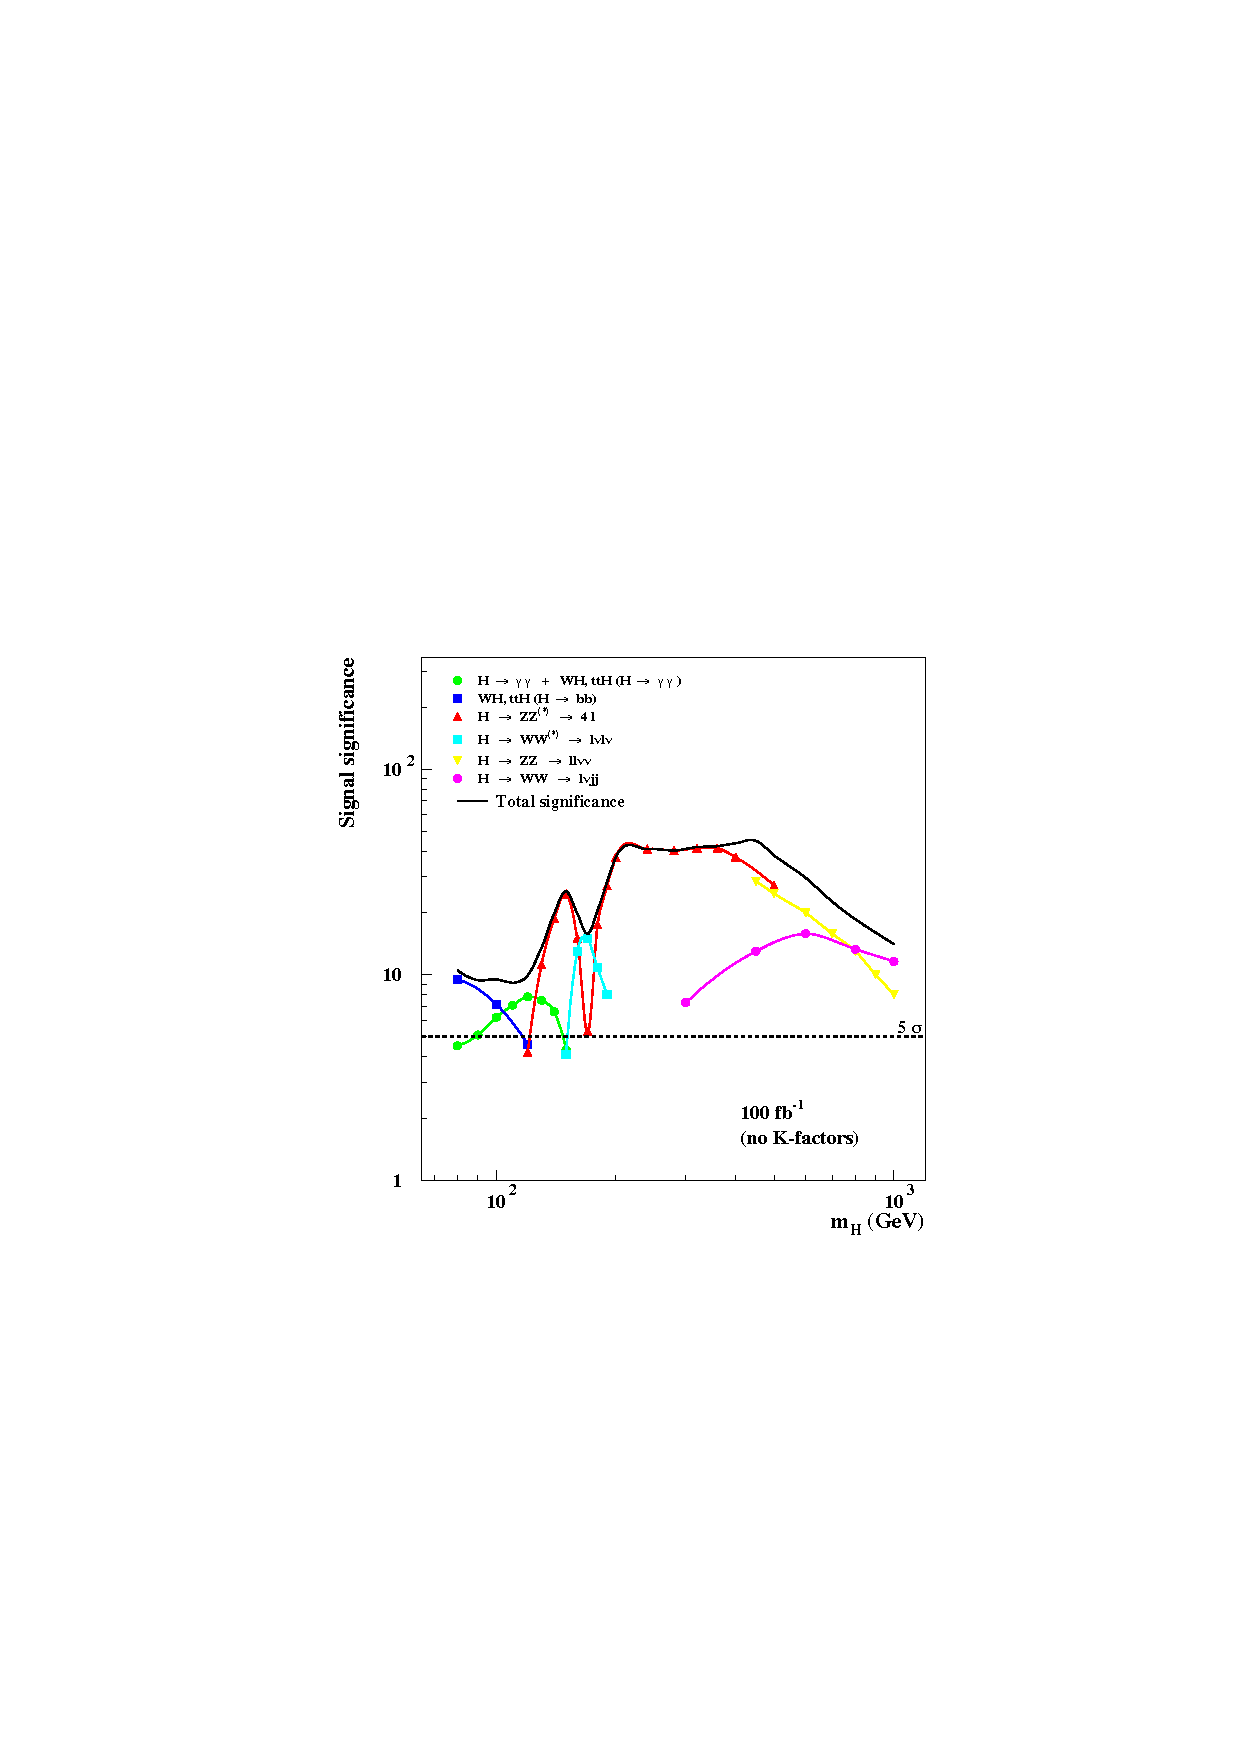
\includegraphics[width=.6\textwidth]{imagens/higgs_sim_atlas.pdf}
        }
    \end{center}
\caption[Simulação da significância dos canais de decaimento do bóssom
de Higgs explorados pelos ATLAS, as relações de seus canais e alcances em massa,
e a seção de choque do mesmo.]
{Os decaimentos do bóssom de Higgs do MP e suas relações de
seus canais e alcances em massa,~\ref{fig:higgs_branch_ratio}, e os seus valores de seção de choque para suas
repectivas massas,~\ref{fig:higgs_production}, ambos extraídas de \cite{lhc_higgs_group}. 
Em \ref{fig:higgs_sim_atlas} está uma simulação da significancia dos possíveis canais de decaimento do
bóssom de Higgs, explorados pelo ATLAS, para uma luminosidade integrada de
$100fb^{-1}$, utilizando as eficiências esperadas para a detecção das
assinaturas dos estados finais e resoluções dos subdetectores, extraído de
\cite{ATLAS_TDR2}.}
\end{figure}

Observe que decaimentos do bóssom de Higgs mais frequentes não são,
necessariamente, os canais com melhor significância esperada. Aqueles canais em
que se tem mais facilidade de observar os decaimentos finais e poder associá-los
a produção de um bóssom de Higgs podem ter mais significância do que canais com
maior produção para uma dada massa. Isso reflete, por outro lado, na importância
dos algoritmos de reconstrução, obtendo melhor eficiência na reconstrução dos
estados finais facilitariam a encontrar o bóssom com menor quantidade de dados.
Os canais mais importantes nas regiões de massa intermediária, $\gls{mh}<2m_Z$,
onde se espera que os decaimentos reconstruam um pico de massa, são 
o canal de quatro léptons, $H\rightarrow ZZ^* \rightarrow 4l$, o canal de
produção direta em dois fótons, $H\rightarrow \gamma\gamma$, junto com os
canais de produção associada com o mesmo estados finais, . Para massas por volta
de 170 GeV/$c^2$, onde a produção de $ZZ^*$ é suprimida, o potêncial da descoberta do
Higgs pode ser elevada pelo decaimento $H\rightarrow WW^*\rightarrow l\nu l\nu$,
nesse caso, o sinal deverá ser observado como um excesso de eventos. O canal de
quatro léptons com dois bóssoms Z reais é o dominante na região de
$\gls{mh}>2m_Z$, cobrindo uma vasta região de massa\footnote{Por isso chegou a
ser referênciado como canal banhado a ouro.}. Em massas mais elevadas, por volta de 600 GeV/$c^2$ até 1
TeV, outros canais como $H\rightarrow WW\rightarrow l\nu jj$, $H\rightarrow
WW\rightarrow ll\nu\nu$ são utilizados para a busca do bóssom de Higgs.

Posteriormente, outro canal foi adicionado, por outros estudos
\cite{atlas_tautau,atlas_tautau2}:

\begin{itemize} 
\item $H\rightarrow \tau \tau \rightarrow ll4\nu$ e $H\rightarrow \tau \tau
\rightarrow l\tau_{had}3\nu$ (110 a 150 GeV/$c^2$), onde $\tau_{had}$ seria o
decaimento do táon em píons especificados no início deste capítulo.
\end{itemize} 

Assim, a reconstrução de elétrons e múons fazem parte de grande
parte dos canais explorados para a vasta região de massa em que se espera
encontrar o bóssom de Higgs, inclusive um dos canais
mais importante por cobrir uma vasta região de massa. Se o Higgs existir com
uma massa mais baixa, os fótons serão necessários para poder encontrar o bóssom,
mostrando a importância do Canal \gls{eg}. 

\begin{figure}[t!]
    \label{fig:higgs_exclusion}
    \begin{center}
    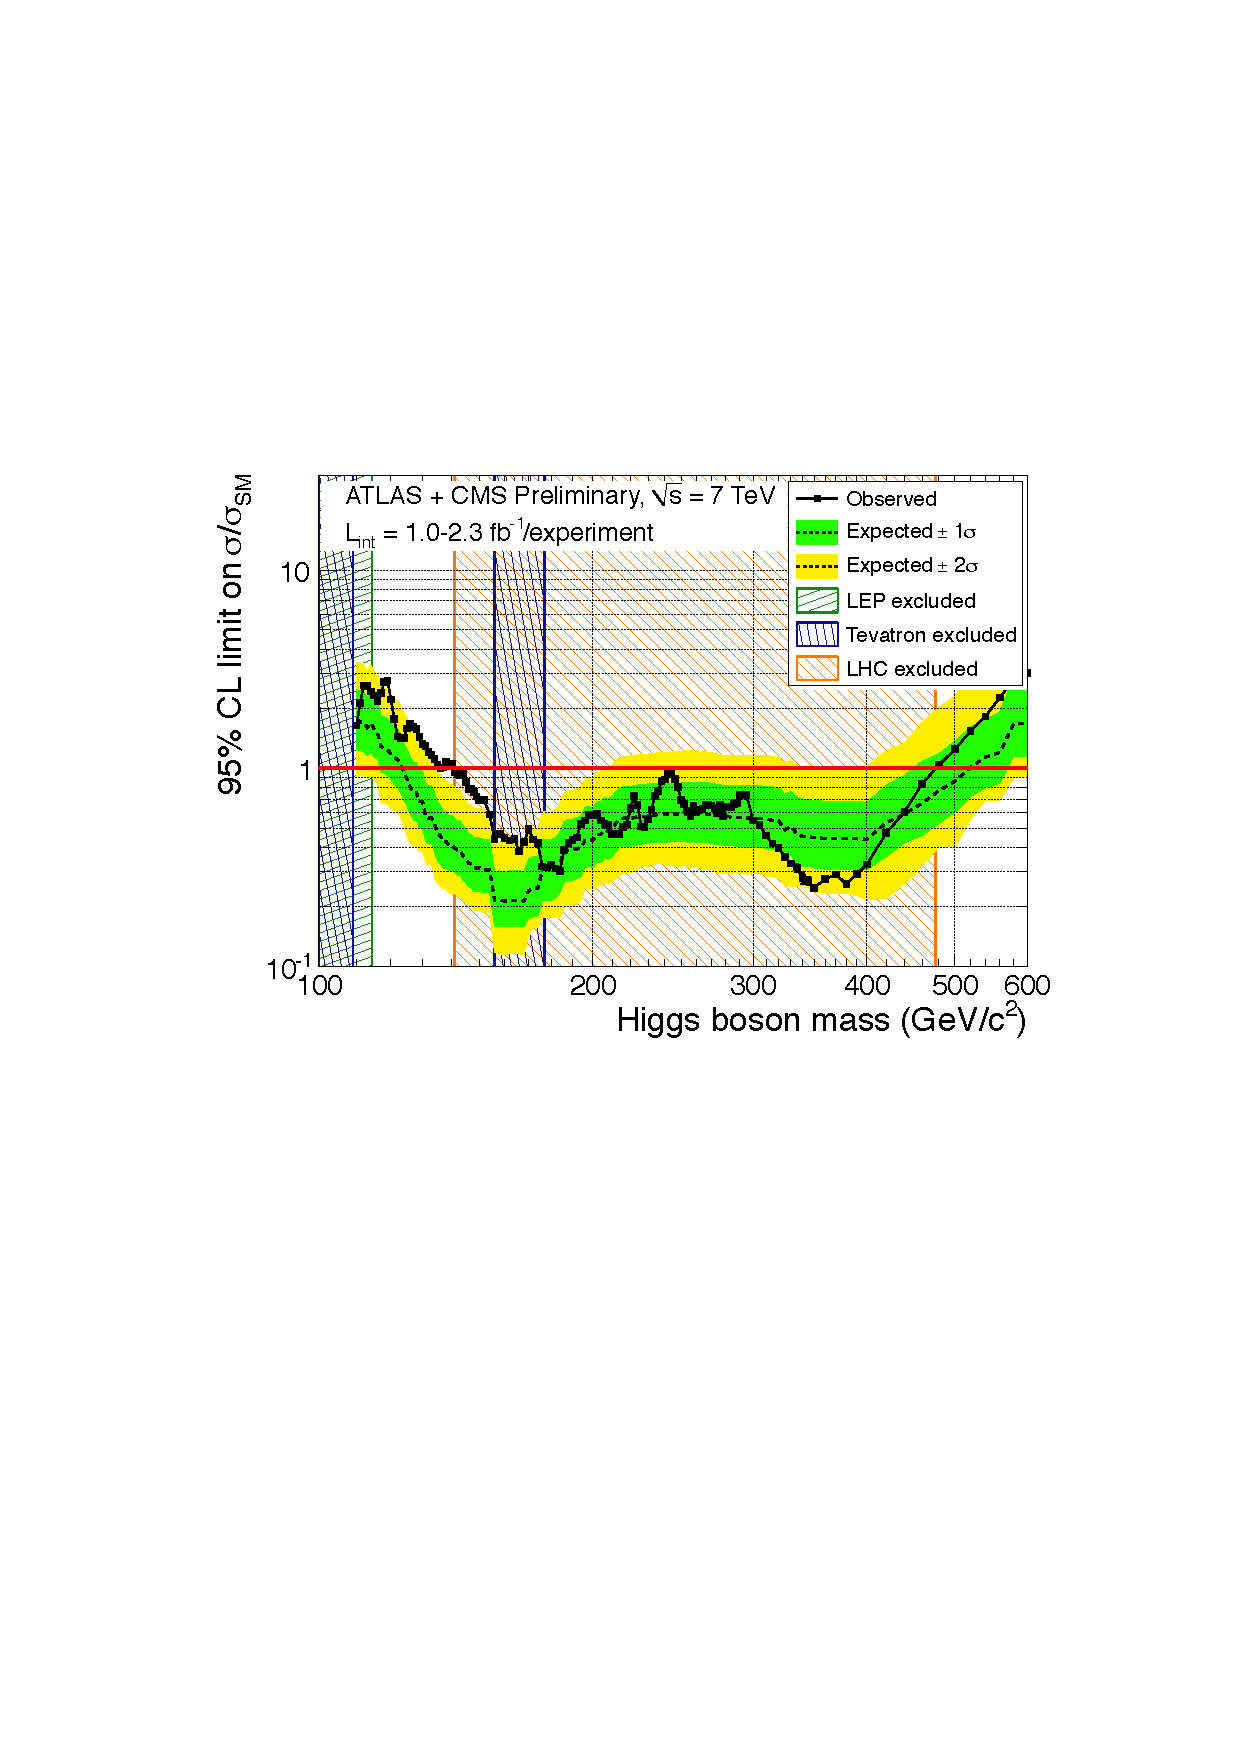
\includegraphics[width=0.8\textwidth]{imagens/exclusion_cms_atlas.pdf}
%
%        \subfigure[LEP, extraído de \cite{lep_higgs_2008}.]{%
%            \label{fig:lep_exclusion}
%            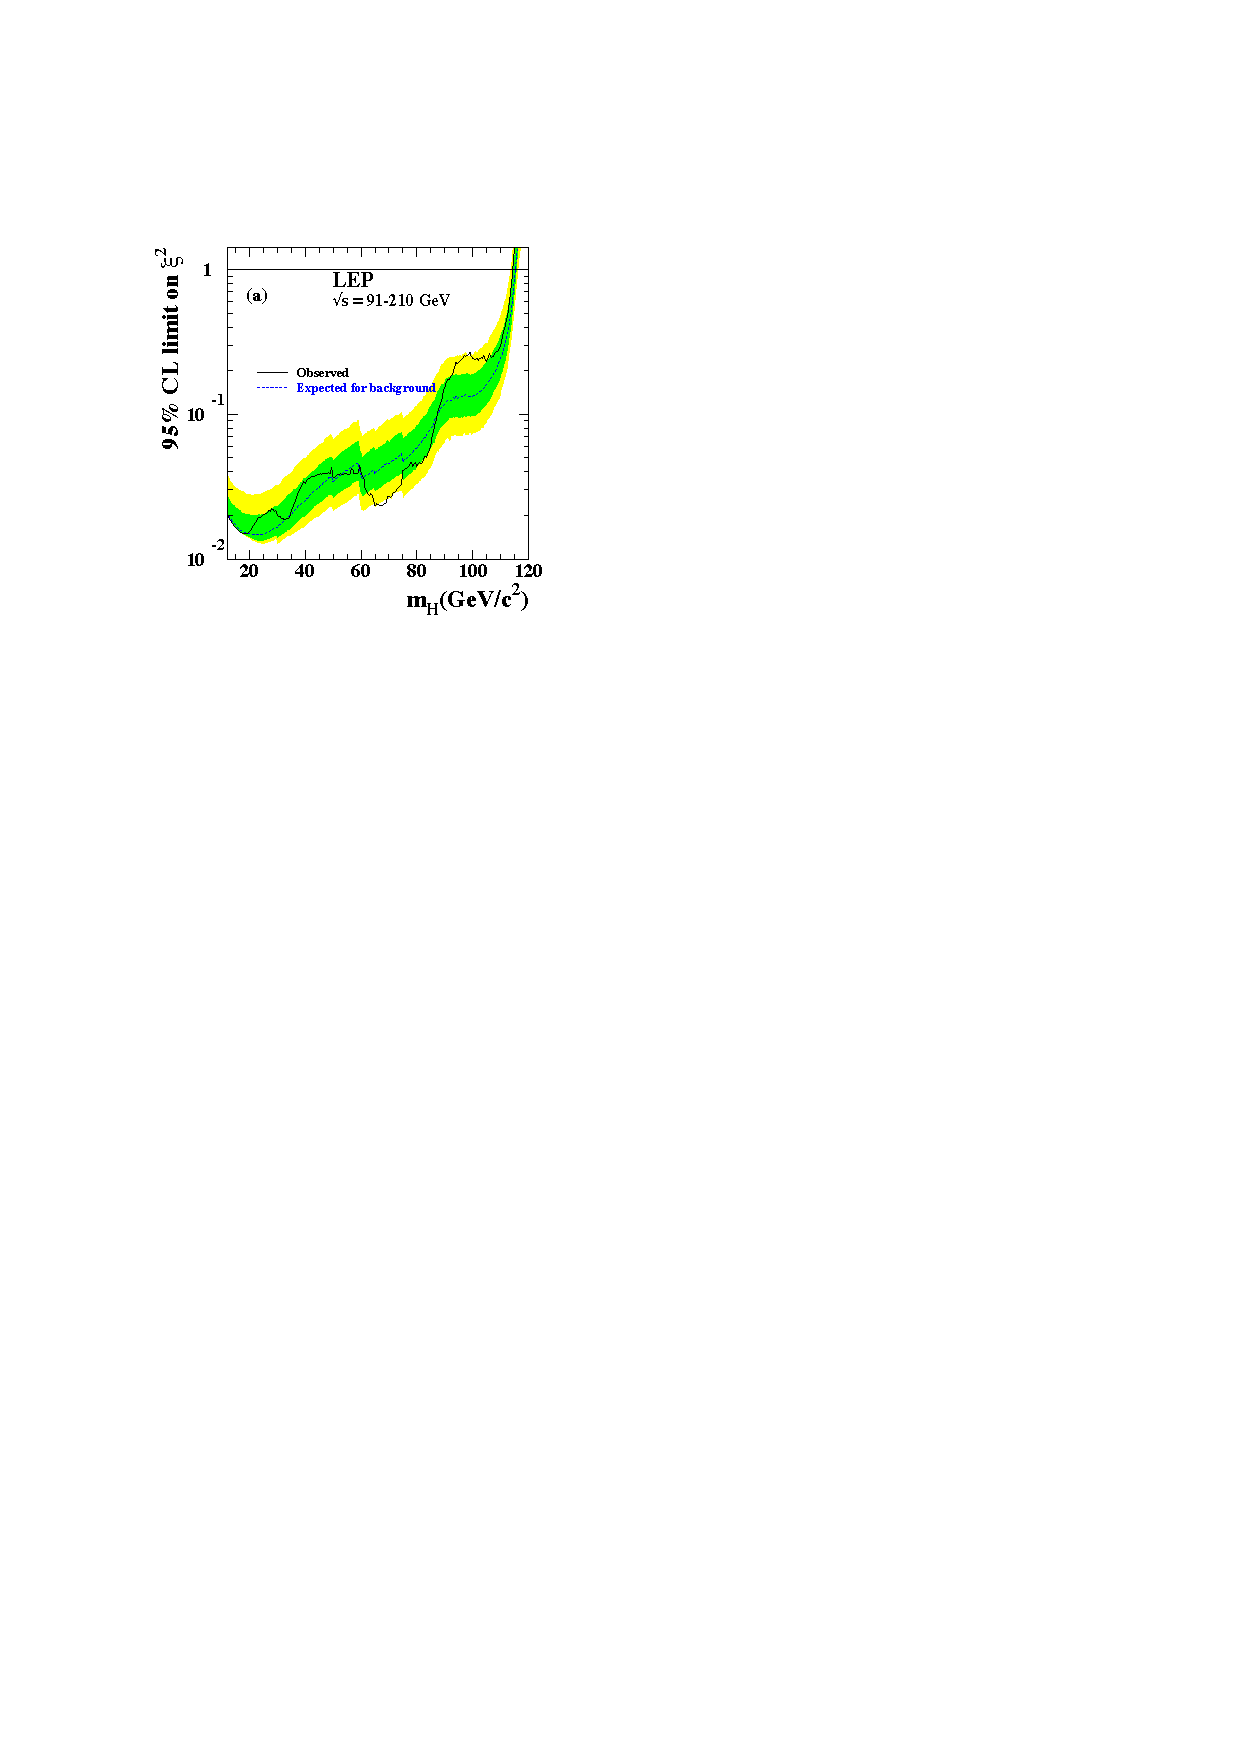
\includegraphics[width=0.47\textwidth]{imagens/lep_exclusion.pdf}
%        }%\hspace{0.1\textwidth}
%        \subfigure[Tevatron, extraído de \cite{tevatron_higgs}.]{%
%            \label{fig:tevatron_exclusion}
%            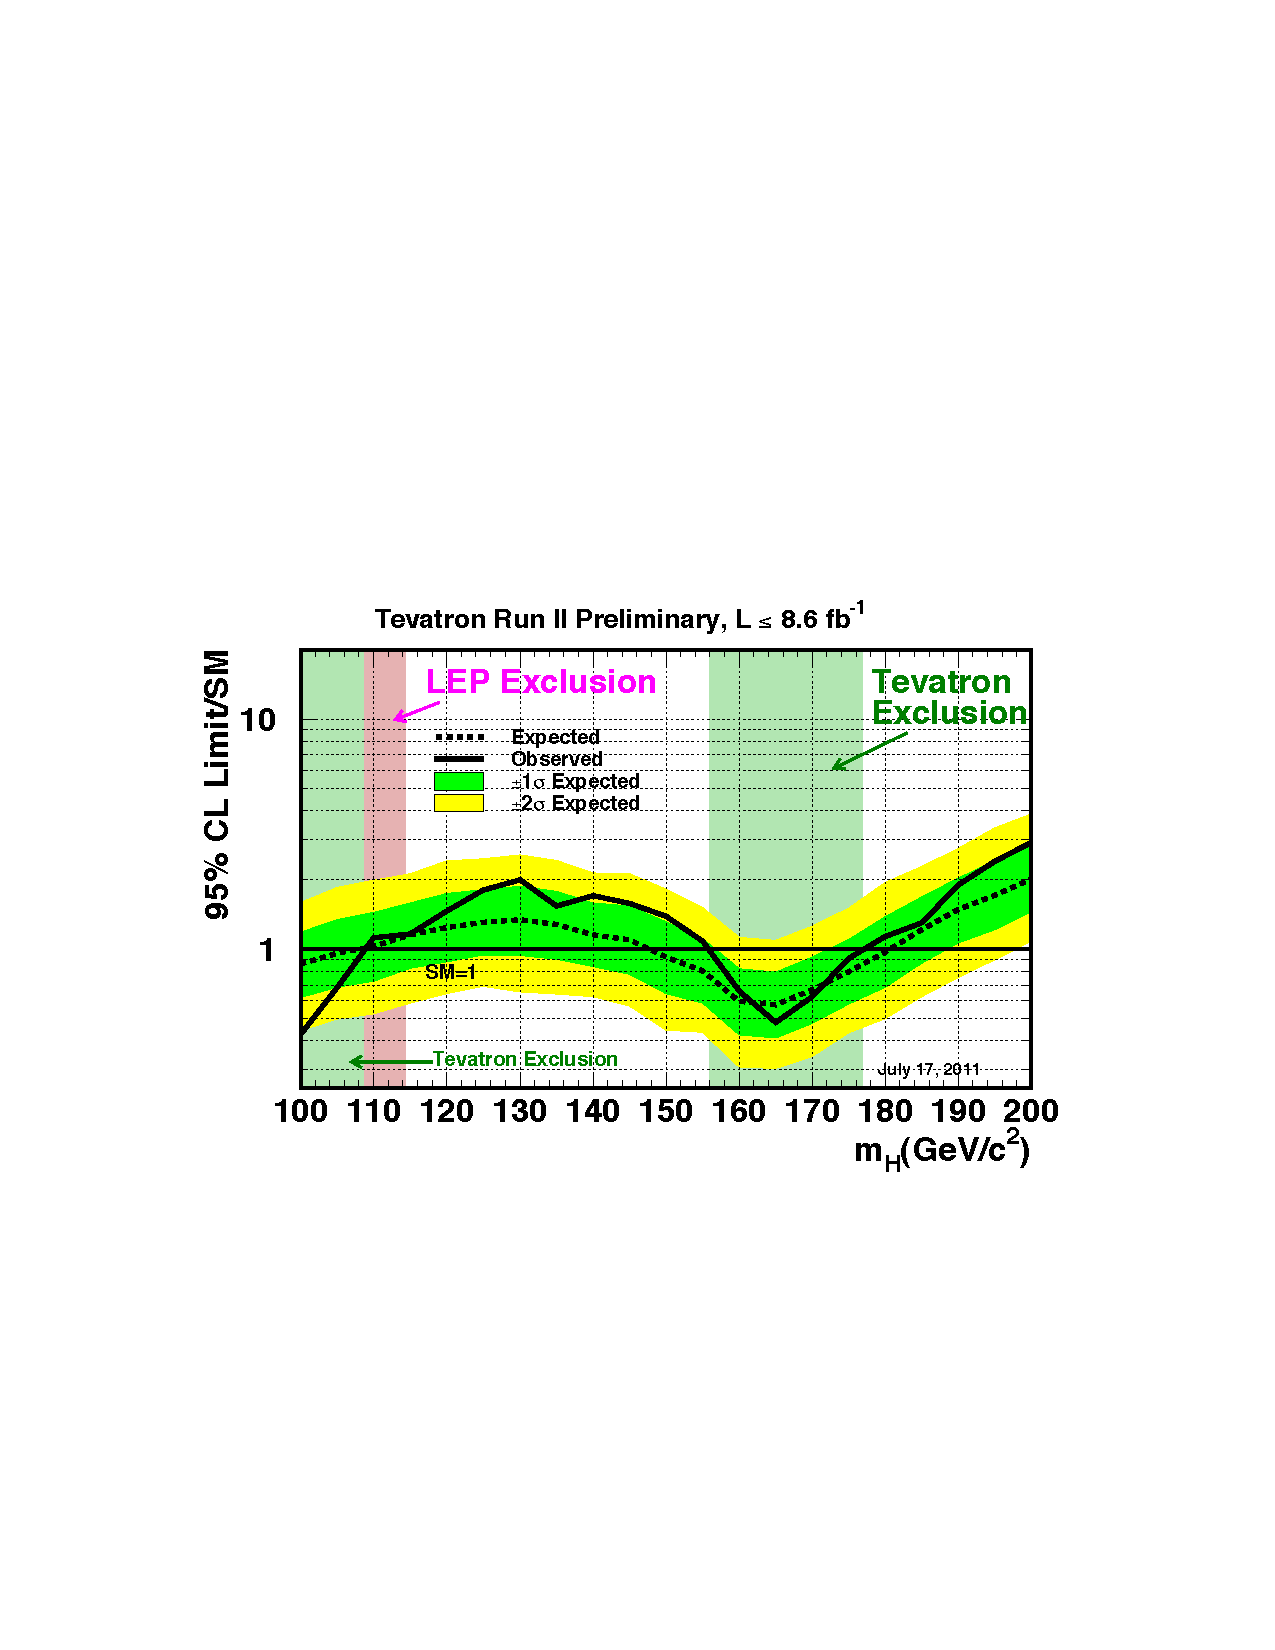
\includegraphics[width=0.47\textwidth]{imagens/tevatron_exclusion.pdf}
%        }\\%\hspace{0.1\textwidth}
%        \subfigure[ATLAS, extraído de \cite{atlas_higgs}.]{
%            \label{fig:atlas_exclusion}
%            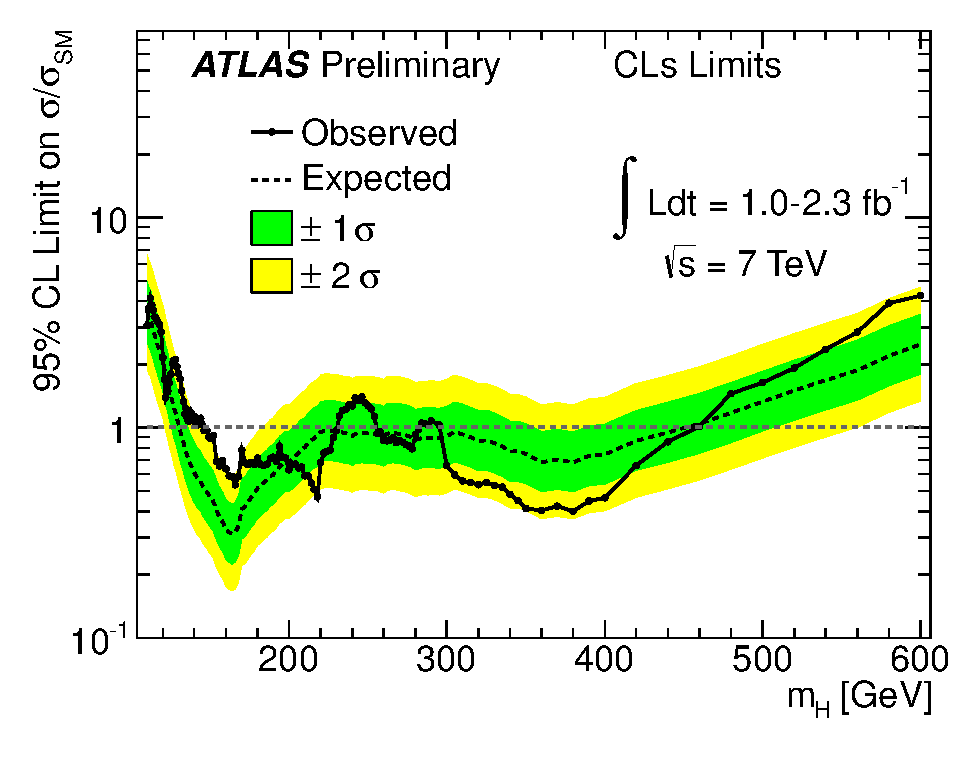
\includegraphics[width=0.47\textwidth]{imagens/atlas_exclusion.pdf}
%        }
%        \subfigure[CMS, extraído de \cite{cms_higgs}.]{%
%            \label{fig:cms_exclusion}
%            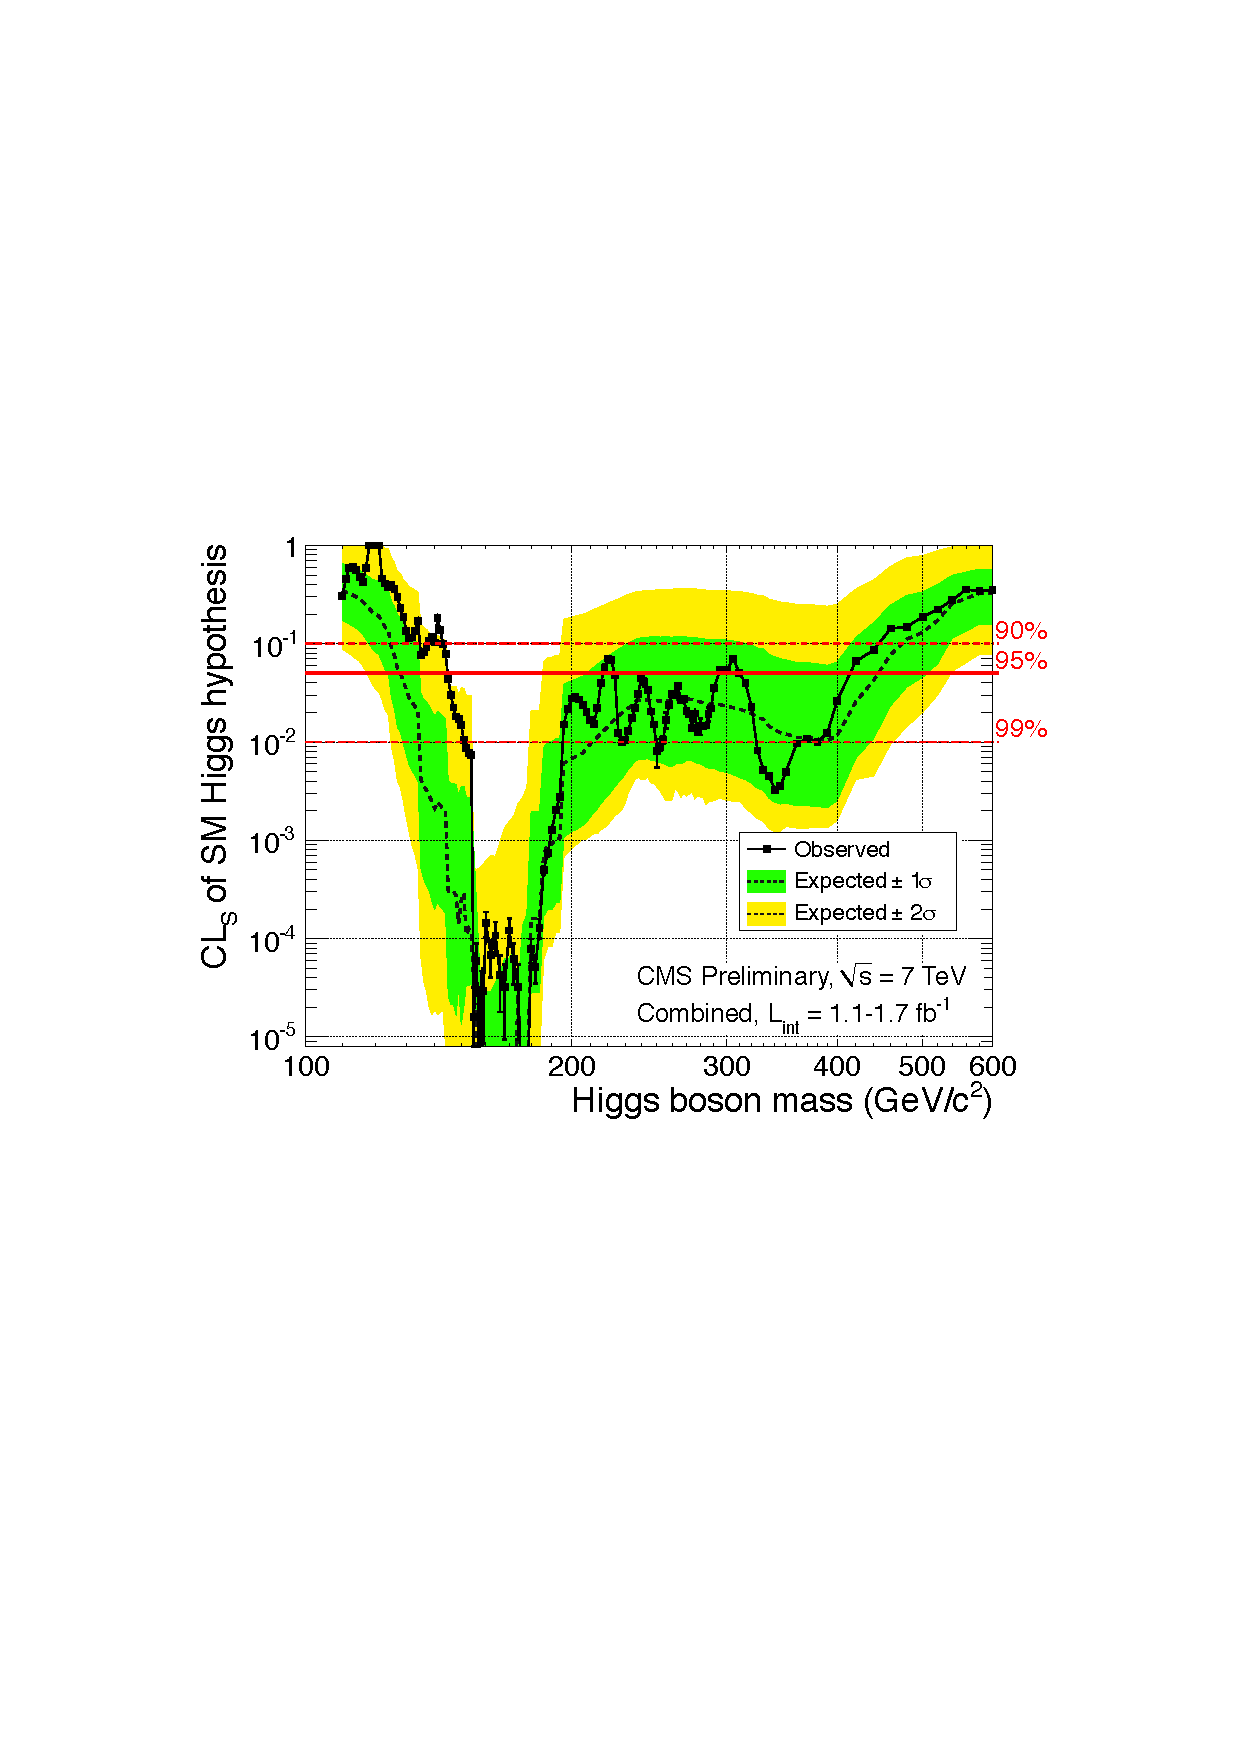
\includegraphics[width=0.47\textwidth]{imagens/cms_exclusion.pdf}
%        }
    \end{center}
\caption[Exclusões de massa do Higgs realizada pela combinação dos dados do
ATLAS e CMS. As exclusões de massa do Tevatron e LEP também estão indicadas.]{As exclusões de massa do bóssom de Higgs. Os valores de massa
observados, no caso para os resultados combinados do ATLAS e CMS, quando
abaixo da linha horizonal vermelha indicada são excluídos com um nível de
confiança de 95\%. A linha pontilhada indica o ruído de fundo esperado gerado
por física na ausência do bóssom de Higgs. As faixas verdes e amarelas indicam
um nível de certeza de 68\% e 95\% de certeza de que algo fora do comum está
ocorrendo. Caso a linha observada ultrapasse o limite superior da faixa amarela
em regiões acima da linha vermelha, então há 95\% de certeza de que há indicios
do bóssom de Higgs ou algum processo de física (talvez ruído físico) não bem
conhecido. Extraído de \cite{atlas_cms_higgs}.}
\end{figure}

Resultados mais recentes excluiram outras regiões de massa do bóssom de Higgs. Em 2008, 
o legado deixado pelo \gls{lep} elevou o limite inferior para 114 GeV/$c^2$
\cite{lep_higgs_2008}, enquanto o experimento Tevatron realizado pelo Fermilab, excluiu as
regiões de $156 < \gls{mh} < 177$ GeV/$c^2$, em Setembro de 2011
\cite{tevatron_higgs}. Também no final de Setembro, resultados preliminares do
\gls{atlas} excluiram o bóssom de Higgs para as regiões de 146-230 GeV/$c^2$, 256-282 GeV/$c^2$ 
e 296-459 GeV/$c^2$ \cite{atlas_higgs}. Um mês antes o \gls{cms} havia excluido o bóssom para
as regiões parecidas: de 145-216 GeV/$c^2$, 226-288 GeV/$c^2$ e 310-400 GeV/$c^2$
\cite{cms_higgs}. Em meados de Novembro o \gls{atlas} e \gls{cms} uniram seus
dados para excluir a região de 141-476 GeV/$c^2$ \cite{atlas_cms_higgs}. Esses
resultados estão indicados na Figura~\ref{fig:higgs_exclusion}, onde estão os
resultados mais recentes do \gls{lhc}, incluidas das regiões anteriormente
excluídas por outros experimentos.


\section{O Sistema de Filtragem (SF)}
\label{sec:sf}

\newacronym[type=Abrev]{asic}{ASIC}{Circuitos Integrados de Aplicação Específica}

O \gls{atlas}, para a luminosidade na qual tem operado: $\sim10^{33}cm^{-2}s^{-1}$,
gera cerca de 19 colisões inelásticas para cada cruzamento entre
feixes, que irão se cruzar numa frequência máxima de 40 MHz. O propósito do
\gls{sf} \cite{trigger_perf_2010,trigger_tdr} é de reduzir essa taxa a cerca
de 200 Hz para seu armazenamento e processamento a posteriori. Esse
limite, correspondendo uma média de $\sim$300 MB/s ($\sim$ 1,5 MB por evento de
cruzamento entre pacotes), é determinado pelos recursos
computacionais para armazenamento e processamento dos dados. É possível gravar
dados com taxas relativamentes mais altas por períodos mais curtos, como foi
realizado durante 2010 quando a física foi beneficiada utilizando taxas de saída
de até $\sim$600 Hz. Nessa época, a luminosidade instantânea máxima atingida foi de
$\sim10^{32}cm^{-2}s^{-1}$, gerando cerca de $\sim$ 1,3 MB, e o \gls{lhc} não 
operava de forma continua -- o que é comum para um acelerador novo -- permitindo 
elevar a taxa de armazenamento.

\subsection{A estrutura do Sistema de Filtragem}
\label{ssec:estru_sf}
\newacronym[type=Abrev]{rob}{ROB}{\emph{Buffer} de Leitura}
\newacronym[type=Abrev]{ros}{ROS}{Sistemas de Leitura}

O \gls{sf}, Figura~\ref{fig:sf_esboco}, é dividido em três níveis sequenciais,
sendo descrito aqui resumidamente uma vez que já foi explicada em maiores detalhes em
trabalhos anteriores como \cite{tese_eduardo,tese_torres}, também podendo ser encontrada 
em detalhes nas referências \cite{trigger_tdr,l1_trigger_tdr,l2_ef_daq_dcs_tdr,trigger_perfomance}.

Os sinais do detector são armazenados em memórias \emph{pipeline}, com pendência
à decisão do \acrshort{l1}. Para obter uma latência de menos de 2,5 $\mu$s, 
o \gls{l1} é implementado em rápida eletrônica constituída de \gls{fpga} e
\gls{asic}, de forma a reduzir a taxa para uma valor máximo de 75 kHz. Para
aumentar a velocidade, esse nível utiliza apenas a informação dos subsistemas de
calorimetria e câmaras de mûons com granularidade reduzida. Além do
primeiro passo de seleção, o \gls{l1} identifica as \glspl{roi} do detector a
serem investigadas pelo \acrshort{hlt}. 

\begin{figure}[ht!]
\label{fig:sf_esboco}
\centering
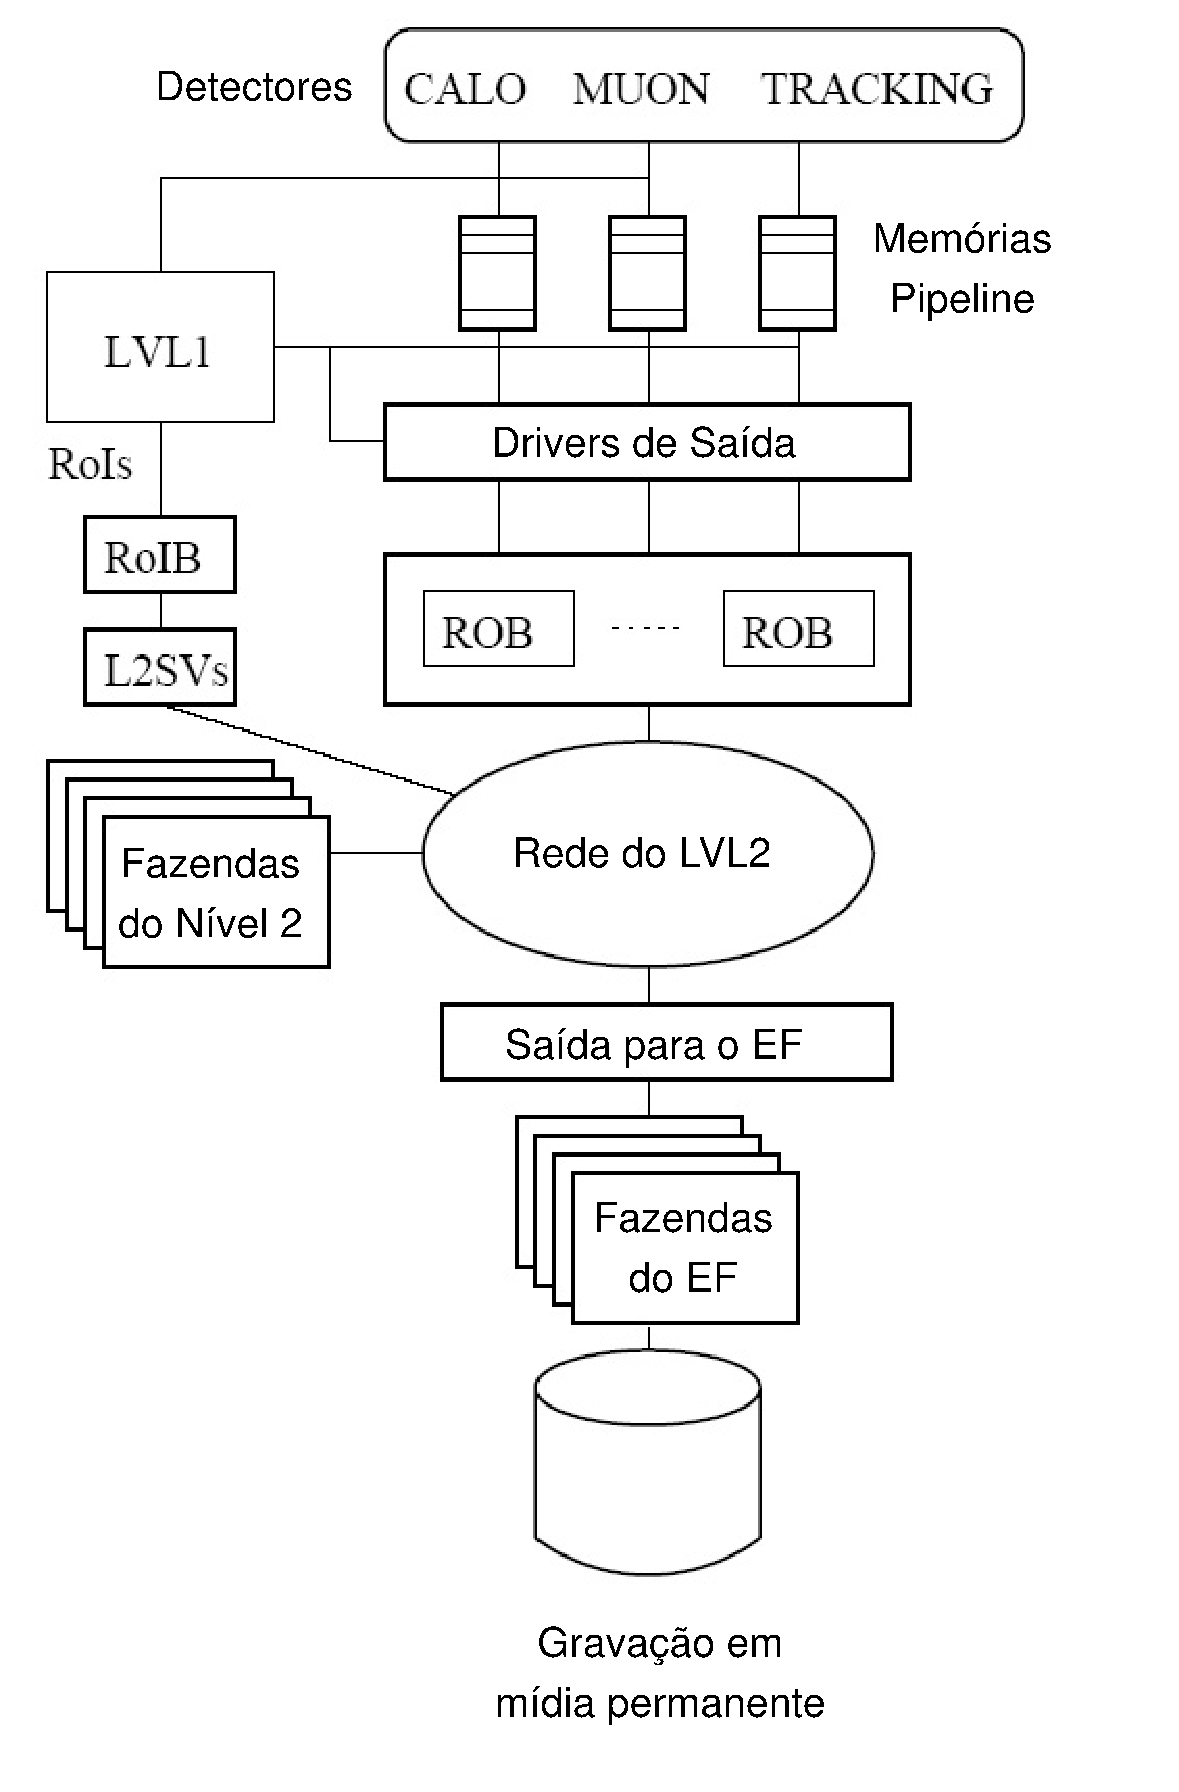
\includegraphics[width=0.6\textwidth]{imagens/sf_resumo.pdf}
\caption[Esboço do Sistema de Filtragem.]{Esboço do Sistema de Filtragem. Extraído de \cite{tese_eduardo}.}
\end{figure}

O \gls{hlt} se consiste de fazendas de
processadores comerciais conectados a rede dedicadas (\emph{Ethernet} de \emph{Gigabit} 
e 10 \emph{Gigabit}).  O \gls{sf} foi projetado para conter cerca de 500 nós para o
\acrshort{l2} e 1800 nós para o \acrshort{ef}\footnote{Em 2010, a fazenda de processamento 
se consistia de 800 nós configuraveis como tanto \acrshort{l2} ou \acrshort{ef}, este 
contendo mais 300 nós dedicados.}. Quando um evento é aceito pelo
\gls{l1}, os dados na memória de cada um dos detectores são então transferidos
para \gls{rob} específicos para cada um dos subdetectores, que armazenam o
evento em fragmentos pendendo à decisão do \gls{l2}. Um ou mais \glspl{rob} são
agrupados para formar os \gls{ros} que são conectados a rede do \gls{hlt}. O
seleção do \gls{l2} é baseada em algoritmos personalizados e rápidos que
processam os dados dos eventos de forma parcial nas regiões especificadas pelas
\glspl{roi} identificadas pelo \gls{l1}. Os processores do \gls{l2} solicitam os
dados dos \gls{ros} correspondentes aelementos do subdetector dentro de cada
\gls{roi}, reduzindo a quantidade de dados a serem transferidas e processadas no
mesmo a cerca de 2-6\% do volume total dos dados. O \gls{l2} reduz a taxa de
dados para cerca de $\sim$3 kHz com uma média de processamento de $\sim$40
ms/evento. Qualquer evento com tempo excedendo a 5 s nesse nível é perdido a
rotulado como evento excedente ao tempo limite.   

O \gls{ef} reune todos os framentos dos eventos aceitos pelo \gls{l2} das
\glspl{rob}, tendo assim acesso a toda sua informação. O \gls{ef} é, em grande
maioria, baseado nos algoritmos do \acrlong{sr} rodando em interfaces
personalizadas para o ambiente do \gls{sf}. Esse nível é projetado para reduzir
os dados para $\sim$200 Hz com uma média de processamento de $\sim$4 s/evento.
Qualquer evento com um tempo excedente a 180 s também é rotulado e perdido como
no \gls{l2}. 

Os eventos de dados selecionados pelo \gls{sf} são escritos nos fluxos de dados
inclusivos, baseados no canal de filtragem. Existem quatro canais de dados
primários, cada um com uma banda pré-determinada (taxa em Hz utilizada na
luminosidade de $10^{32}cm^{-2}s^{1}$): Egamma (50),
Muons (50), JetTauEtMiss (65), Minbias (10), adicionados de diversos canais
de calibração (13). Cerca de 10\% dos eventos são escritos 
para um canal expresso aonde a reconstrução pronta dos eventos é realizada, como foi dito na
Subseção~\ref{ssec:lcg}. Ainda, além da gravação de evnetos completos em um
canal, é possível escrever informação parcial de um ou mais subdetectores em um
canal, o que é normalmente realizado para a calibração do detector nos canais
destinados a esse propósito.


\subsection{Topologia dos algoritmos e sua configuração}
\label{ssec:alg_topo}

\newacronym[type=Abrev,\glslongpluralkey={Algoritmos de Extração de
Características}]{fex}{FEX}{Algoritmo de Extração de Característica}
\newacronym[type=Abrev,\glslongpluralkey={Algoritmos de Hipótese}]
{hypo}{HYPO}{Algoritmo de Hipótese}

A configuração do \gls{sf} é realizada por um \emph{menu}, que define as
\emph{cadeias} de filtragem que especificam uma sequência de passos de reconstrução e
seleção para as especificas assinaturas de filtragems requeridas pela filtragem.
A cadeia de filtragem de elétrons é ilustrada na Figura~\ref{fig:electron_chain}.
Cada \emph{cadeia} é composta pelo \gls{fex} que criam objetos,
como os aglomerados de células e variáveis que permitam obter uma informação
sobre a descrição do evento, e pelo \gls{hypo} que fazem a discriminação através dos
critérios de seleção nos objetos gerados, como por exemplo a exigência de um
$\gls{pt} > 20$ GeV. As extrações de características realizadas por uma
\emph{cadeia} podem ser reutilizadas por outro cadeia, reduzindo tanto o acesso
a dados como o tempo de processamento do \gls{sf}.

\begin{figure}[ht!]
\label{fig:electron_chain}
\centering
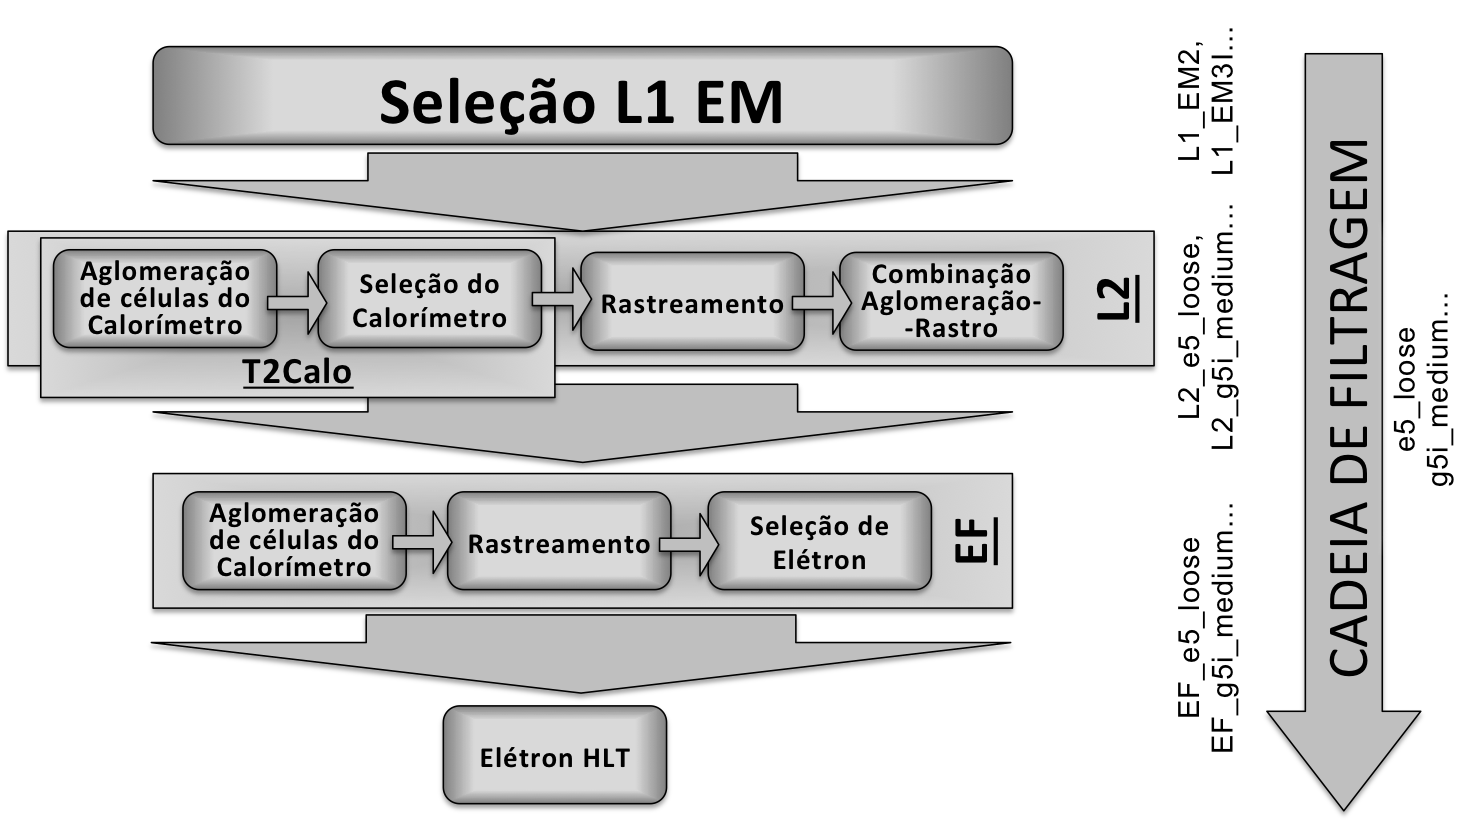
\includegraphics[width=0.9\textwidth]{imagens/cadeia_eletron.png}
\caption[A \emph{cadeia} de filtragem de elétrons.]{A \emph{cadeia} de filtragem
de elétrons. A direita de cada nível de filtragem estão colocados exemplos de
nomes de filtros de elétrons e fótons, e o nome de sua respectiva cadeia a
direita da seta indicando a evolução da \emph{cadeia}. Adaptado de \cite{trigger_perf_2010}.}
\end{figure}

Aproximadamente 500 filtros são definidos nos \emph{menus} atuais, sendo
composto por um número de diferentes classes de filtros:

\begin{enumerate}
\item \textbf{Objetos de filtro único}: usado para determinar estados com pelo
menos um objeto característico. Por exemplo, um filtro para elétron único com um
limiar nominal superior a 3 GeV seria referido como $e3$;
\item \textbf{Objetos de filtro multiplos}: usado para determinar estados finais
com dois ou mais objetos do mesmo tipo. Por exemplo, elétrons duplos decaindo da
partícula $\text{J}/\Psi$. Esses filtros são indicados dependendo de sua
multiplicidade, por exemplo: $2e3$;
\item \textbf{Objetos de filtro combinados}: usados por estados finais de dois
ou mais objetos característicos de tipos diferentes. Por exemplo, um múon de 13
GeV adicionado de 20 GeV de \gls{Etmiss} para selecionar decaimentos
$W\rightarrow \mu\nu$, que seriam denotados de $mu13\_xe20$;
\item \textbf{Filtros Topológicos}: usados para estados finais selecionados de
duas ou mais \glspl{roi}, como no caso do decaimento da partícula
$\text{J}/\Psi$, que combina os traços das duas \glspl{roi} provenientes dos
elétrons.
\end{enumerate}

Quando se referindo a um nível em partícular, o nível (\gls{l1}, \gls{l2},
\gls{ef}) aparece como um prefixo, como por exemplo L1\_EM3 (aqui elétrons e
fótons não são diferenciados, então se utiliza o prefixo EM em ambos os casos)
para denotar um filtro de elétrons e fótons com um limiar nominal superior a 3
GeV para o \gls{l1} e L2\_e3 no caso de elétrons para um filtro com o mesmo
limiar mas para elétrons apenas no \gls{l2}. Um nome sem o prefixo de nível
refere-se a toda a \emph{cadeia}.

O controle das taxas de filtragem podem ser realizadas mudando os limiares ou
aplicando outros valores de seleção. A seletividade de um grupo de cortes
aplicados para um certo objeto de filtragem é representado pelos termos
\emph{Loose} (relaxado), \emph{Medium} (mediano), \emph{Tight} (apertado). Esses
critérios de seleção são colocados como sufixos ao nome do filtro, por exemplo,
e10\_medium. Requerimentos adicionais como isolamento, podem ser adicionados
para reduzir as taxas dos filtros. O isolamento mede a quantidade de energia, ou
o número de partículas próximos a uma assinatura, se esse valor estiver acima de
um limiar, então a partícula não está isolada. Nesse caso se adiciona a letra
'i' ao nome do filtro, como por exemplo L1\_EM20I ou e20i\_tight.

Fatores de \emph{pré-escala} podem ser adicionados a cada filtro da 
\emph{cadeia} do \gls{hlt}, de tal forma que apenas 1 em cada N eventos passando
o filtro causam que o evento seja aceito por aquele nível. A \emph{pré-escala}
controla a taxa e composição dos canais expressos. Uma série de
\emph{pré-escalas} são utilizadas baseadas em diversas regras que levam em
consideração a prioridade dos filtros em relação com as seguintes categorias:

\begin{enumerate}
\item \textbf{Filtros Primários}: filtros princípais de física, que não deveriam
ser \emph{pré-escalados};
\item \textbf{Filtros de Suporte}: filtros importantes de suporte a filtros
primários, como filtros que permitam estudar a eficiência utilizando 
seletividades mais baixas e limiar mais baixo de \gls{Et} \emph{pré-escalados}
para permitir sua gravação em disco, uma vez que a quantidade de dados que
passam esse filtro será maior;
\item \textbf{Filtros de Monitoração e Calibração}: permitindo a coleta de dados
para garantir a operação correta do \gls{sf} e dos subdetectores do \gls{atlas},
incluindo a calibração dos mesmos. 
\end{enumerate}

\newacronym[type=Abrev]{lb}{LB}{Bloco de Luminosidade} 

Esses fatores de \emph{pré-escala} devem ser modificados conforme a queda da
luminosidade durante um preenchimento do \gls{lhc} de forma a garantir a
maximização das taxas utilizadas pelos filtros, enquanto garantindo uma taxa
constante para a monitoração e calibração. Assim, as mesmas podem ser alteradas
em quaisquer momentos de uma temporada, no início de um novo \gls{lb}. Um
\gls{lb} é a unidade fundamental para a medição da luminosidade, cerca de 120 s
em 2010, na qual se considera que a mesma permaneceu constante com o valor
medido.

Flexibilidade adicional é oferecida ao definir \emph{grupos de pacotes}, separando os
filtros para colisões com pacotes emparelhados (compõe as colisões de física
regulares, contendo pacotes de feixes opostos que se encontram no ponto de
colisão simultaneamente), pacotes vazios para estudo de pedestal criado por ruído 
no detector e raios cósmicos, ou até mesmo configurações mais inusitadas, como 
exigindo pacotes desparelhados separados por no mínimo 75 ns de quaisquer outro 
pacote no feixe oposto.



\subsection[Algoritmos Padrões da \emph{Cadeia} de Filtragem de eGamma]{Algoritmos Padrões da \emph{Cadeia} de Filtragem de $e/\gamma$}
\label{ssec:cadeia_egamma}

\newacronym[type=Abrev,\glslongpluralkey={Torres de Filtragem}]
{tt}{TT}{Torre de Filtragem}

O sistema de calorimetria do \gls{atlas} cobre uma região de $|\gls{eta}| <
4,9$, enquanto o \gls{id} fornece reconstrução precisa de traços dentro de
$|\gls{eta}| < 2,5$. Os chuveiros \gls{em} são reconstruídos com melhor
performance para essa última região, a região de precisão do \gls{atlas}, 
contendo calorímetros com maior granularidade como descrito na
Subseção~\ref{ssec:calorimetria}. Assim, os filtros de elétrons e fótons
\cite{expected_perf_2011,perf_2011} do \gls{sf} atuam somente para essa região.
A cadeia de elétrons no \gls{sf} está esboçada na Figura~\ref{fig:electron_chain}, entretanto
a cadeia de fótons pode ser facilmente extrapolada ao se remover os algoritmos
referentes ao \gls{id}.

No \gls{l1}, os aglomerados de informação\footnote{No caso, um conjunto de
células identificados como \emph{clusters} na literatura em inglês.} \gls{eg} do calorímetro são retirados
utilizando granularidade reduzida, as chamadas \glspl{tt}, que cobrem uma região
de aproximadamente $\Delta\eta\times\Delta\phi\approx0,1\times0,1$, 
a Figura~\ref{fig:cal_lar_camadas} contem um esboço da \gls{tt} para o
\gls{emb}. A vantagem de se utilizar \glspl{tt} se deve ao
fato de reduzir a quantidade de fluxo de informação, reduzindo o custo e
complexidade do sistema, e, ao mesmo tempo, conter o chuveiro \gls{em} inteiramente 
em cerca de uma ou duas dessas torres, podendo
assim identificar a região em que foi formado o chuveiro não prejudicando a sua
eficiência. Para cada \gls{tt}, as células do \gls{ecal} e \gls{hcal} são somadas, com a
excessão da quarta camada do \gls{hec} e dos cintiladores.
Um algoritmo de janela deslizante formada por uma dimensão de $4\times4$
\gls{tt}, ilustrada na Figura~\ref{fig:sliding_window_l1}, 
busca pela região com a melhor deposição de energia do chuveiro por
todo o calorímetro com um passo de uma \gls{tt}.
O \gls{l1} seleciona o evento como um candidato a \gls{eg} 
quando os seguintes critérios forem satisfeitos:

\begin{figure}[ht!]
\label{fig:l1_alg}
\centering
        \subfigure[A janela deslizante, seu núcleo e as regiões de isolamento.]{
            \label{fig:sliding_window_l1}
            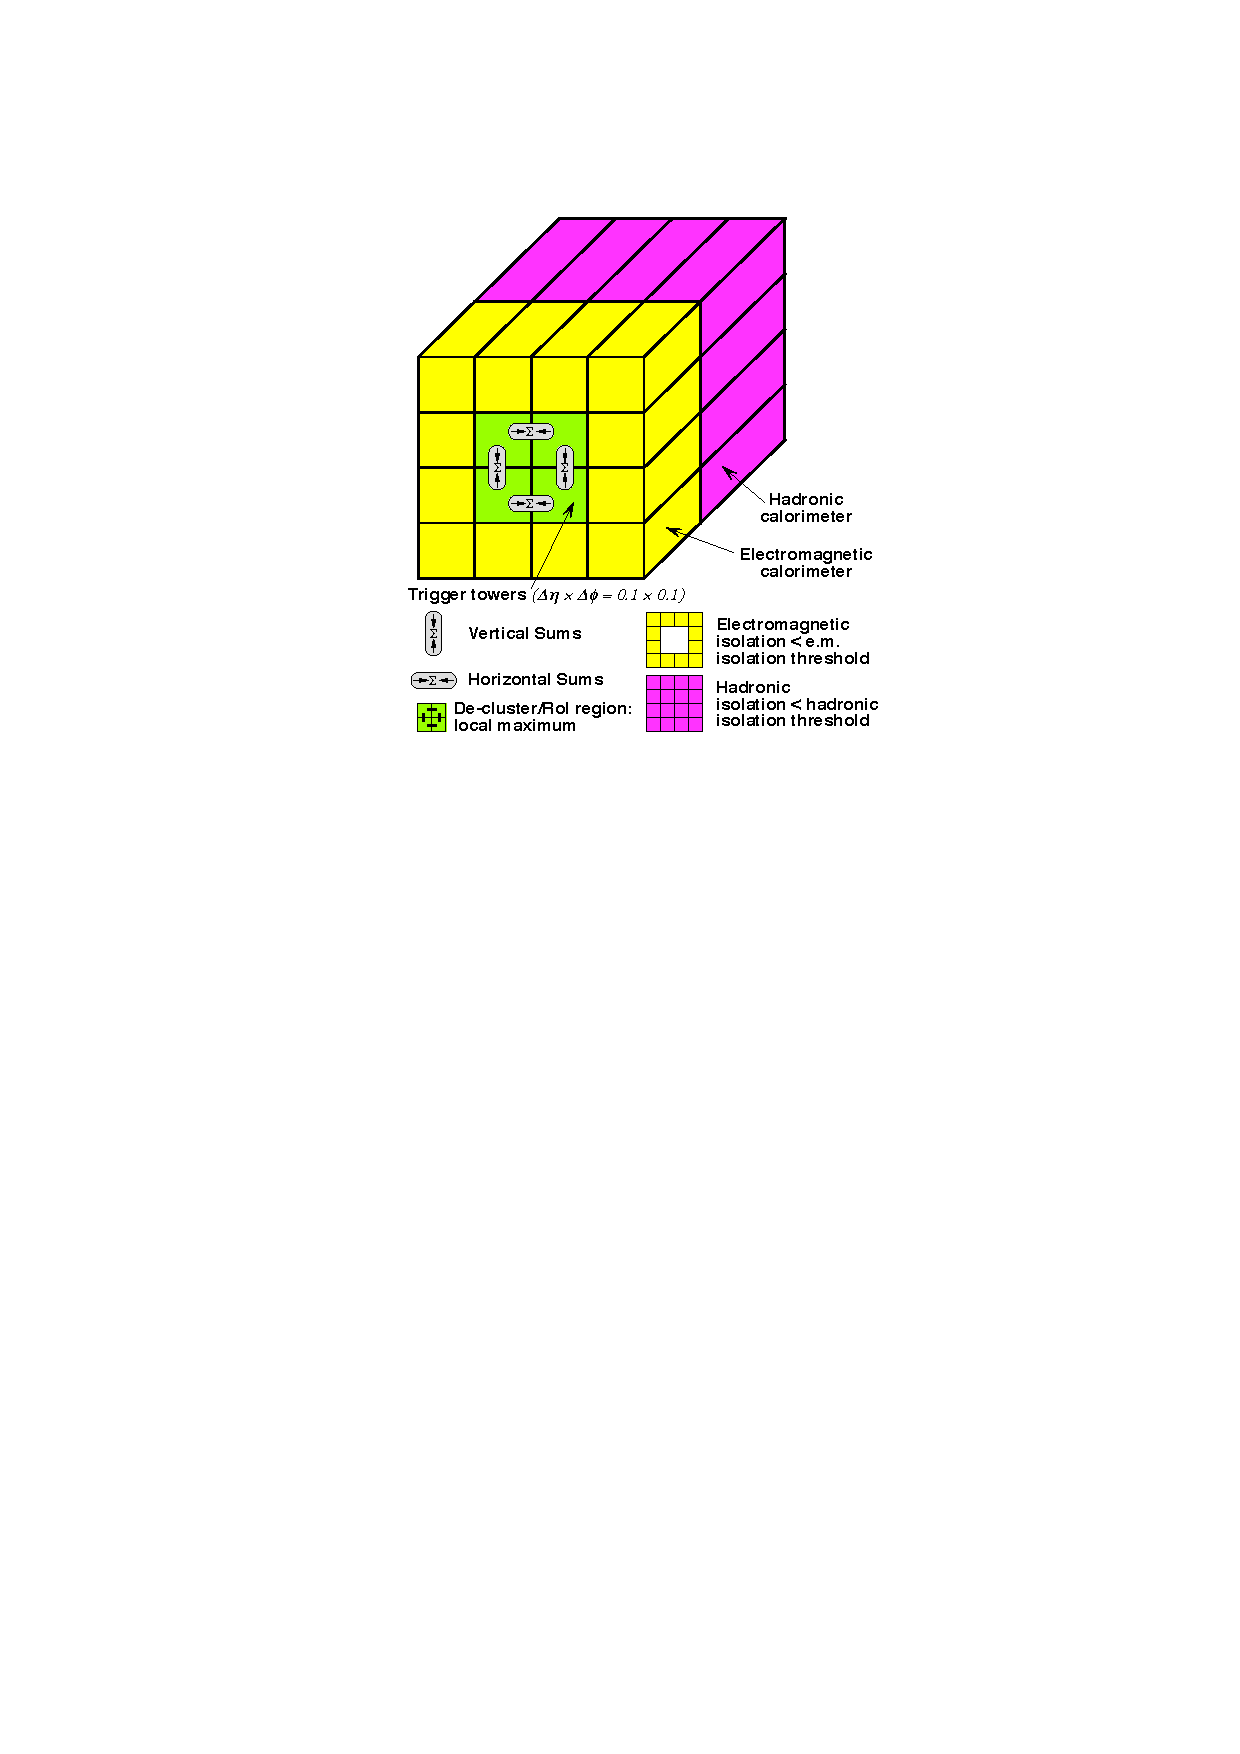
\includegraphics[width=0.6\textwidth]{imagens/sliding_window_l1.pdf}
        }\hspace{0.01\textwidth}
        \subfigure[Requerimento para o núcleo ser máximo local.]{%
            \label{fig:local_et}
            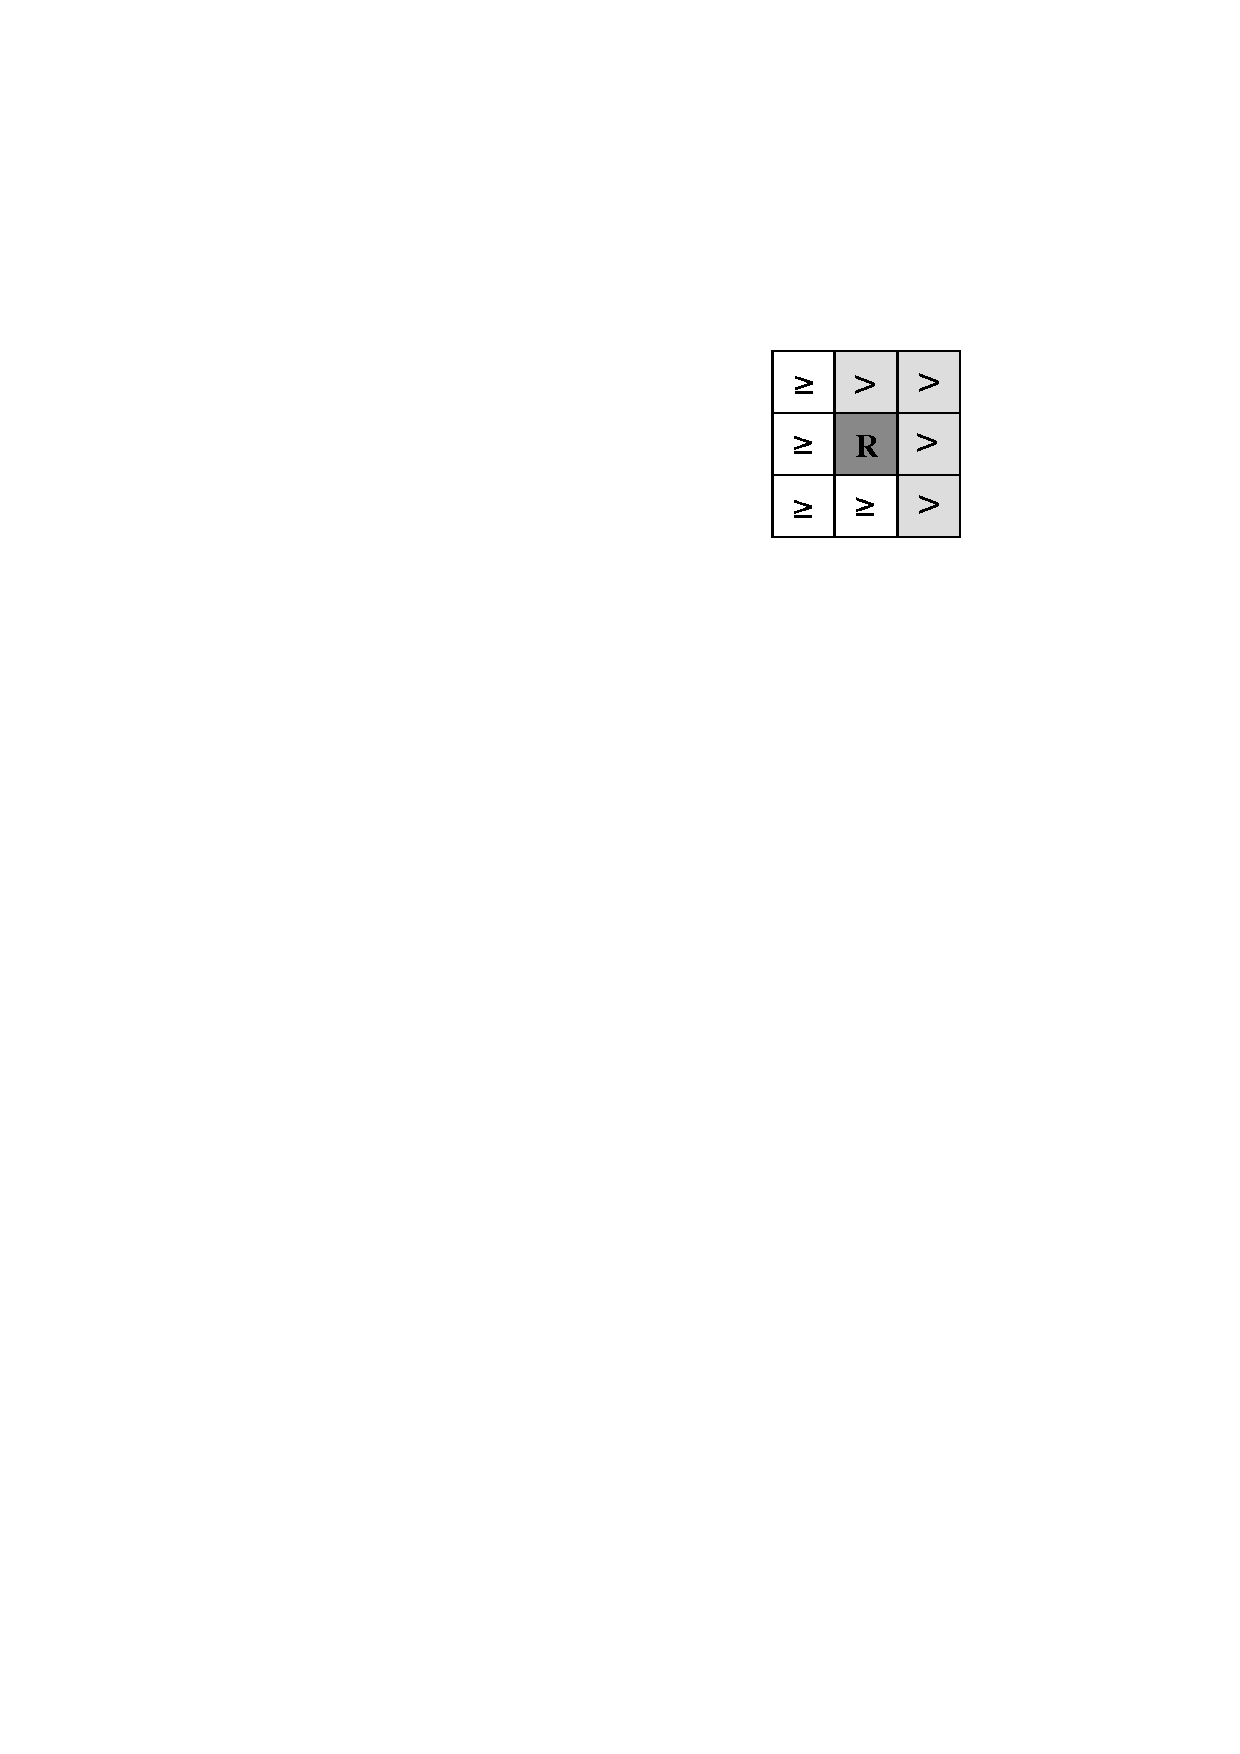
\includegraphics[width=0.3\textwidth]{imagens/roi_local_max.pdf}
        }
\caption[O Primeiro Nível de Filtragem para a Cadeia de Elétrons e Fótons.]
{O Primeiro Nível de Filtragem para a Cadeia de Elétrons e Fótons. Extraído de
\cite{l1_trigger_tdr}.}
\end{figure}

\begin{itemize}
\item A região deve ser um máximo local. Essa condição é importante para se
evitar multiplicidade de \glspl{roi} a serem analisadas pelo \gls{l2}.
Assim, a energia contida no núcleo deve ser
maior, ou ao menos igual, como na lógica da Figura~\ref{fig:local_et}, 
que em todos as outras regiões de $2\times2$ que podem ser formados na
janela;
\item O aglomerado formado pela dupla de torre mais energética na região
(indicados na Figura~\ref{fig:sliding_window_l1} como somas verticais ou horizontais) deve ultrapassar o limiar
\gls{em} exigido pelo filtro do \gls{l1}. A posição de \gls{eta} e \gls{phi} desse aglomerado é passado
para o \gls{l2}, junto com outros \emph{bits} indicando os critérios que foram
satisfeitos, que formarão a palavra informada para o \gls{l2} para a qual será
utilizada para a formação da \gls{roi};
\item Se isolamento for exigido: 
\begin{itemize}
\item A \gls{Et} total da região \gls{em} de
isolamento não deve ultrapassar o limiar de isolamento \gls{em};
\item A \gls{Et} total da região \gls{had} de isolamento não deve ultrapassar o
limiar de isolamento \gls{had}.
\end{itemize}
\end{itemize}


O \gls{l2}, alimentado pela posição dos
aglomerados de torres do \gls{l1}, realiza uma rápida reconstrução do
calorímetro, e no caso de elétrons, uma rápida reconstrução dos traços no \gls{id}. A
reconstrução do calorímetro trabalha de maneira semelhante aos algoritmos do
\gls{sr}, entretanto apenas a região da janela de $\Delta\eta\times\Delta\phi =
0,4 \times 0,4$, região chamada de \gls{roi}, em torno da posição alimenda pelo \gls{l1} 
é utilizada, o que reduz o tráfico de dados e aumenta a velocidade de processamento no \gls{l2}.
Algumas diferenças entre o algoritmo do \gls{l2} e o \gls{sr} se dão as
limitações no tempo de latência. O algoritmo de reconstrução do aglomerado de
células do calorímetro no \gls{l2} começa utilizando a célula mais energética da
\gls{e2} dentro da região central de $0,2 \times 0,2$, enquanto o
algoritmo de análise a posteriori utiliza uma janela deslizante para encontrar
sua semente.

No \gls{l2}, o tamanho do aglomerado é fixado para $3
\times 7$ células em $\gls{eta} \times \gls{phi}$ para o barril ($|\gls{eta}|<1,5$) e 
$5 \times 5$ na tampa ($1,5<|\gls{eta}|<2,5$). O algoritmo a posteriori possui
tamanhos diferentes dependendo do tipo de partícula e se a incidência foi no
barril ou na tampa. No caso de incidência no barril, elétrons são reconstruídos
através de aglomerados com $3\times7$ torres; fótons $3\times5$, 
e fótons convertidos em elétrons, $3\times7$. Na tampa todos os aglomerados 
são de $5\times5$.

As energias das células podem ser corrigidas na análise a posteriori, para
problemas transientes no \emph{hardware}, como falhas de energia, etc., o que não
pode ser realizado em tempo real, o que se aplica para tanto o \gls{l2} e
\gls{ef}. Para a reconstrução de traços no \gls{l2}, um rápido reconhecimento de
padrões é utilizado ao se determinar primeiro a posição z de interação ao longo
do eixo do feixe e então realizando a combinação de pontos do traço apenas para o grupo
de pontos que apontam para a posição determinada. O traço com a menor distância
$\Delta R$, definida por \ref{eq:dist_clust_traco}, será atribuido ao
aglomerado e seus parâmetros utilizados pelo \gls{l2} para a discriminação.

\begin{equation}\label{eq:dist_clust_traco}
\Delta R = \sqrt{\Delta'2\eta+\Delta^2\phi}
\end{equation}

Como no \gls{sr}, a reconstrução do aglomerado no \gls{ef} é realizado
utilizando um algoritmo de janela deslizante que será
explicado em \ref{ssec:egamma}. Basicamente, após encontrada
a semente através do máximo local, um aglomerado é construido iniciando da \gls{e2},
com o mesmo tamanho que aqueles descritos para o algoritmo a posteriori. O
centro de distribuição de energia em \gls{eta} e \gls{phi} é calculado
utilizando o aglomerado construido na \gls{e2}, e então o valor dessa
posição é propagado de forma a incluir as camadas faltantes. O algoritmo
de reconstrução de traços é feito como no algoritmo a posteriori, com uma
combinaçao dos traços começando dos pontos dos Detectores de Silicone e
\gls{trt}.

Os algoritmos de seleção são aplicados na reconstrução do
\gls{l2} e no \gls{ef} com o objetivo de identificar bons candidatos a \gls{eg}
e rejeitar falsos alarmes provenientes de jatos. As seleções são baseadas no
formato do chuveiro nas aglomerações, tentando identificar as diferenças já
citadas entre os chuveiros \gls{em} e \gls{had} no
Subtópico~\ref{par:cal_part_id}, como: a largura dos chuveiros, onde os \gls{em}
devem ser mais estreitos; sua profundidade, no qual os \gls{had} são mais
profundos que os \gls{em} para uma partícula de mesma energia e geralmente
somente os \gls{had} deverão alcançar o \gls{hcal}, ou deverão
depositar a maior parte de sua energia no calorímetro específico para a
contenção de sua energia. Para elétrons, também se utiliza critérios de seleção 
baseados em informação do traço e qualidade de casamento entre o aglomerado e o
traço. A parte do algoritmo responsável pela reconstrução do calorímetro no
\gls{l2} é chamada de \emph{T2Calo}.

\newacronym[type=Simb]{Rhad1}{\ensuremath{R_{had1}}}{Variável de corte dos
algoritmos \acrshort{eg} padrões. Ver tabela \ref{tab:cortes_em}} 
\newacronym[type=Simb]{Rhad}{\ensuremath{R_{had}}}{Variável de corte dos
algoritmos \acrshort{eg} padrões. Ver tabela \ref{tab:cortes_em}} 
\newacronym[type=Simb]{reta}{\ensuremath{R_{\eta}}}{Variável de corte dos
algoritmos \acrshort{eg} padrões. Ver tabela \ref{tab:cortes_em}} 
\newacronym[type=Simb]{eratio}{\ensuremath{E_{ratio}}}{Variável de corte dos
algoritmos \acrshort{eg} padrões. Ver tabela \ref{tab:cortes_em}} 
\newacronym[type=Simb]{weta2}{\ensuremath{w_{\eta2}}}{Variável de corte dos
algoritmos \acrshort{eg} padrões. Ver tabela \ref{tab:cortes_em}} 
\newacronym[type=Simb]{wstot}{\ensuremath{w_{stot}}}{Variável de corte dos
algoritmos \acrshort{eg} padrões. Ver tabela \ref{tab:cortes_em}} 
\newacronym[type=Simb]{deta1}{\ensuremath{\Delta\eta_1}}{Variável de corte dos
algoritmos \acrshort{eg} padrões. Ver tabela \ref{tab:cortes_em}} 
\newacronym[type=Simb]{dphi2}{\ensuremath{\Delta\phi_2}}{Variável de corte dos
algoritmos \acrshort{eg} padrões. Ver tabela \ref{tab:cortes_em}} 
\newacronym[type=Simb]{Ep}{\ensuremath{\frac{E}{p}}}{Variável de corte dos
algoritmos \acrshort{eg} padrões. Ver tabela \ref{tab:cortes_em}} 

\glsunset{Rhad1}
\glsunset{Rhad}
\glsunset{eratio}
\glsunset{reta}
\glsunset{wstot}
\glsunset{weta2}
\glsunset{deta1}
\glsunset{dphi2}
\glsunset{Ep}

Os três conjuntos de requerimentos citados em~\ref{ssec:alg_topo} são utilizados para 
seleção de partículas \gls{eg}. Eles são definidos ao se elevar a potência de rejeição 
de ruído físico nos dados finais: \emph{Loose}, com menor seletividade, 
evitando a perda de dados prematura, mas ao mesmo tempo elevando a taxa de dados 
a serem gravados; \emph{Tight}, com grande seletividade, reduzindo o
ruído físico e a taxa de dados, mas podendo haver perda de eventos de interesse;
\emph{Medium}, que concilia a escolha da seletividade de forma
a reduzir a taxa de armazenamento ao mesmo tempo que evita a perda de eventos
de forma prematura. As variáveis utilizadas no \gls{ef}, dispostas na
Tabela~\ref{tab:cortes_em}, são as mesmas que as
utilizadas na versão a posteriori, mas com limiares tipicamente mais relaxados
que no último para se evitar a perda de eventos interessantes, enquanto o
\gls{l2} utiliza apenas algumas dessas variáveis, novamente com valores mais relaxados que no 
\gls{ef} pelo mesmo motivo. No caso do \gls{t2calo} essas variáveis são: \gls{reta}, 
\gls{eratio}, \gls{Et} e \gls{Rhad1}, com algumas condições específicas 
dependendo da região em que a partícula está incidindo, em especial nesse 
caso para a região de fenda do calorímetro, e para partículas de altas energias onde se aceita um maior
vazamento hadrônico. Os valores dos limiares são escolhidos através de estudos
de \gls{mc}, e, ainda que os mesmos variem conforme \gls{eta} e a energia da
partícula, eles são compostos por diversos cortes lineares nessas variáveis
físicas. Vale ressaltar que as variáveis utilizando o \gls{id} 
não se aplicam para fótons, independente do algoritmo em questão.


\begin{table}
\centering
\resizebox{\textwidth}{!}{
\begin{tabular}{p{4cm}p{9cm}c}
\hline
\hline
\hline
\textbf{Tipo} & \textbf{Descrição} & \textbf{Símbolo (se aplicável)} \\
\hline
\hline
 & \centering Cortes \emph{Loose} & \\
\hline
\hline
Vazamento Hadrônico & Razão de \gls{Et} da primeira camada \gls{had} com a
depositada no \gls{ecal} (usado para $|\gls{eta}|<0,8$ e
$|\gls{eta}|>1,37$). & \gls{Rhad1} \\
 & Razão de \gls{Et} da energia depositada no \gls{hcal} com a
depositada no \gls{ecal} (usado para $|\gls{eta}|>0,8$ e
$|\gls{eta}|<1,37$). & \gls{Rhad} \\
\hline
\gls{e2} & Razão em \gls{eta} entre a enegia contida nas
células numa região de $3\times7$ por uma região $7\times7$. & \acrshort{reta}\\
 & Largura lateral do chuveiro. & \gls{weta2} \\
\hline
\hline
 & \centering Cortes \emph{Medium} (Incluem o \emph{Loose}) & \\
\hline
\hline
\gls{e1} & Largura total do chuveiro. & \gls{wstot} \\
 & Diferença entre o primeiro e o segundo depósito de maiores
energias normalizadas por sua soma. & \gls{eratio} \\
\hline
Qualidade do Traço & Número de pontos no Detector de Píxel ($\ge1$). & \\
 & Número de pontos no Detector de Píxel e \gls{sct} ($\ge7$). & \\
 & Parâmetro de impacto transverso ($<5$ mm). & \gls{d0} \\
\hline
Casamento de Traço & $\Delta\eta$ entre o aglomerado de células e traço (<0,01)
& \\
\hline
\hline
 & \centering Cortes \emph{Tight} (Incluem o \emph{Medium}) & \\
\hline
\hline
Primeira Camada do Detector de Pixel (Camada B) & Número de pontos na camada B
($\ge1$).  & \\
\hline
Casamento de Traço & $\Delta\phi$ entre o aglomerado de células e traço
(<~0,02). & \gls{dphi2} \\
 & Razão entre a energia do aglomerado com o momento medido pelo \gls{id}. & \gls{Ep} \\
 & Corte mais restritivo em $\Delta\eta$ (<~0,005). & \gls{deta1} \\
\hline
Qualidade do Traço & Parâmetro de impacto transvero mais restritivo (<~1 mm).  & \gls{d0} \\
\hline
\gls{trt} & Número de pontos no \gls{trt}. & \\
 & Razão entre o número de pontos de alto limiar pelo número total de pontos para o
\gls{trt}. & \\
\hline
Conversões & Candidatos a elétron provenientes de fótons convertidos são
rejeitados. & \\
\hline
\hline
\end{tabular}
}
\caption[Definições dos cortes utilizados para os critérios de identificação de elétrons \emph{loose}, \emph{medium}
e \emph{tight}, na região de $|\eta|<2,47$]
{Definições dos cortes utilizados para os critérios de identificação de elétrons \emph{loose}, \emph{medium}
e \emph{tight}, na região de $|\gls{eta}|<2,47$. Adaptado de \cite{expected_perf_2011}.}
\label{tab:cortes_em}
\end{table}

Cada uma dessas variáveis contribuem na discriminação de acordo com os critérios
de corte utilizados. Na Figura~\ref{fig:cortes_egamma_padrao} estão dispostos a
distribuição nas variáveis de corte dos algoritmos padrão utilizados na
colaboração para dados de simulações de \gls{mc} separados nas seguintes 
categorias \cite{expected_perf_2011}:

\begin{itemize}
\item Elétrons isolados: elétrons originados de decaimentos dos
bóssoms W ou Z, ou outras partículas como o $\text{J}/\Psi$;
\item Hádrons: os hádrons provenientes de
jatos hadrônicos compondo ruído físico para o Canal \gls{eg};
\item Elétrons não-isolados: elétrons
provenientes de mésons-b(c). Elétrons não-isolados têm sua distribuição
comprometida, uma vez que são formados por elétrons dentro de jatos;
\item Elétrons constituintes de ruído: elétrons
provenientes de decimentos \emph{Dalitz} ou provenientes de fótons. Os elétrons
provenientes de fótons podem ser divididos dependendo da origem do fóton, por
exemplo, o fóton pode ser gerado de um decaimento de um $\pi^0$, ou de um
chuveiro \gls{em} de um elétron originados de um decaimento de um Z, ou da
radiação de estado inicial ou final de um bóssom Z.
\end{itemize}

\begin{sidewaysfigure}[p]
\centering
        \subfigure[\protect\acrshort{Rhad1}.]{%
            \label{fig:Rhad1}
            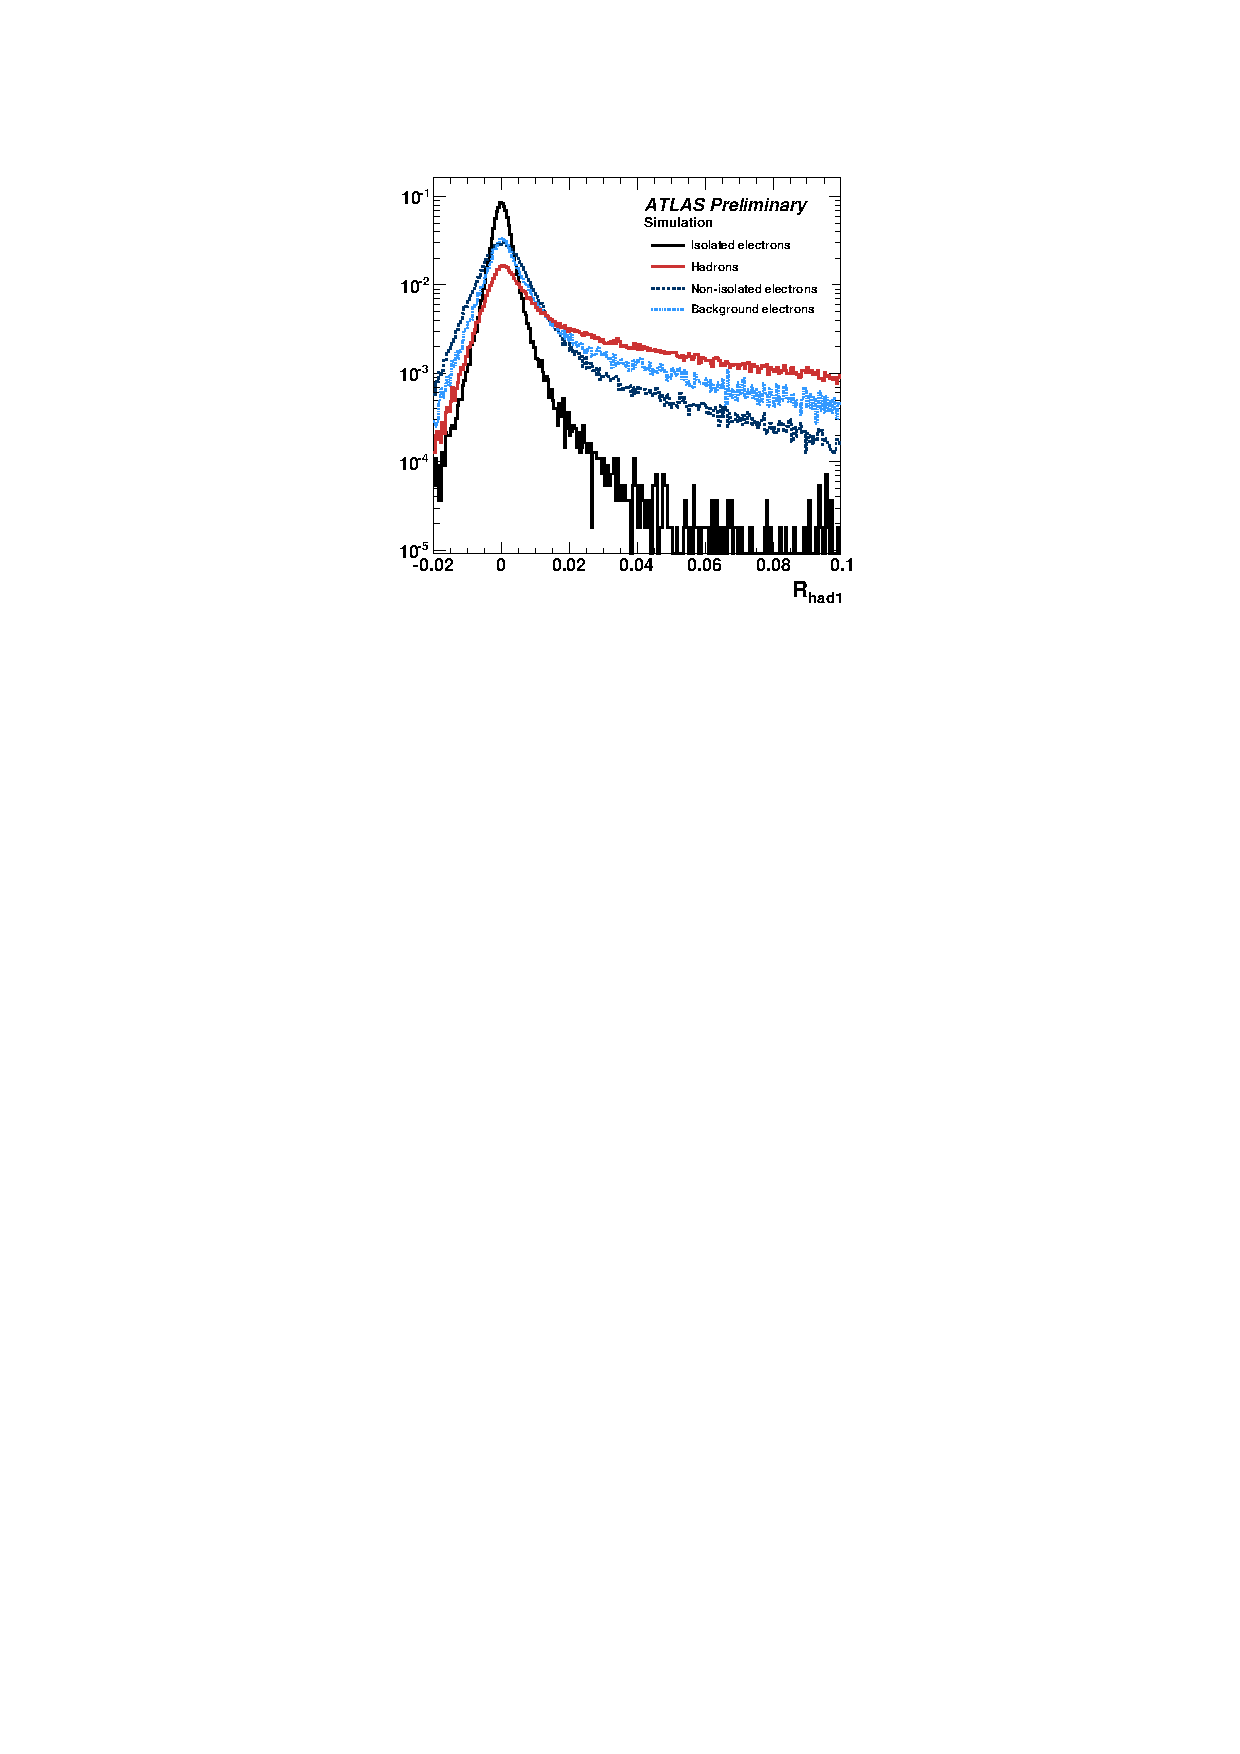
\includegraphics[width=0.2\textwidth]{imagens/egamma_padrao/egamma_padrao_rhad1.pdf}
        }
        \subfigure[\protect\acrshort{weta2}.]{%
            \label{fig:weta2}
            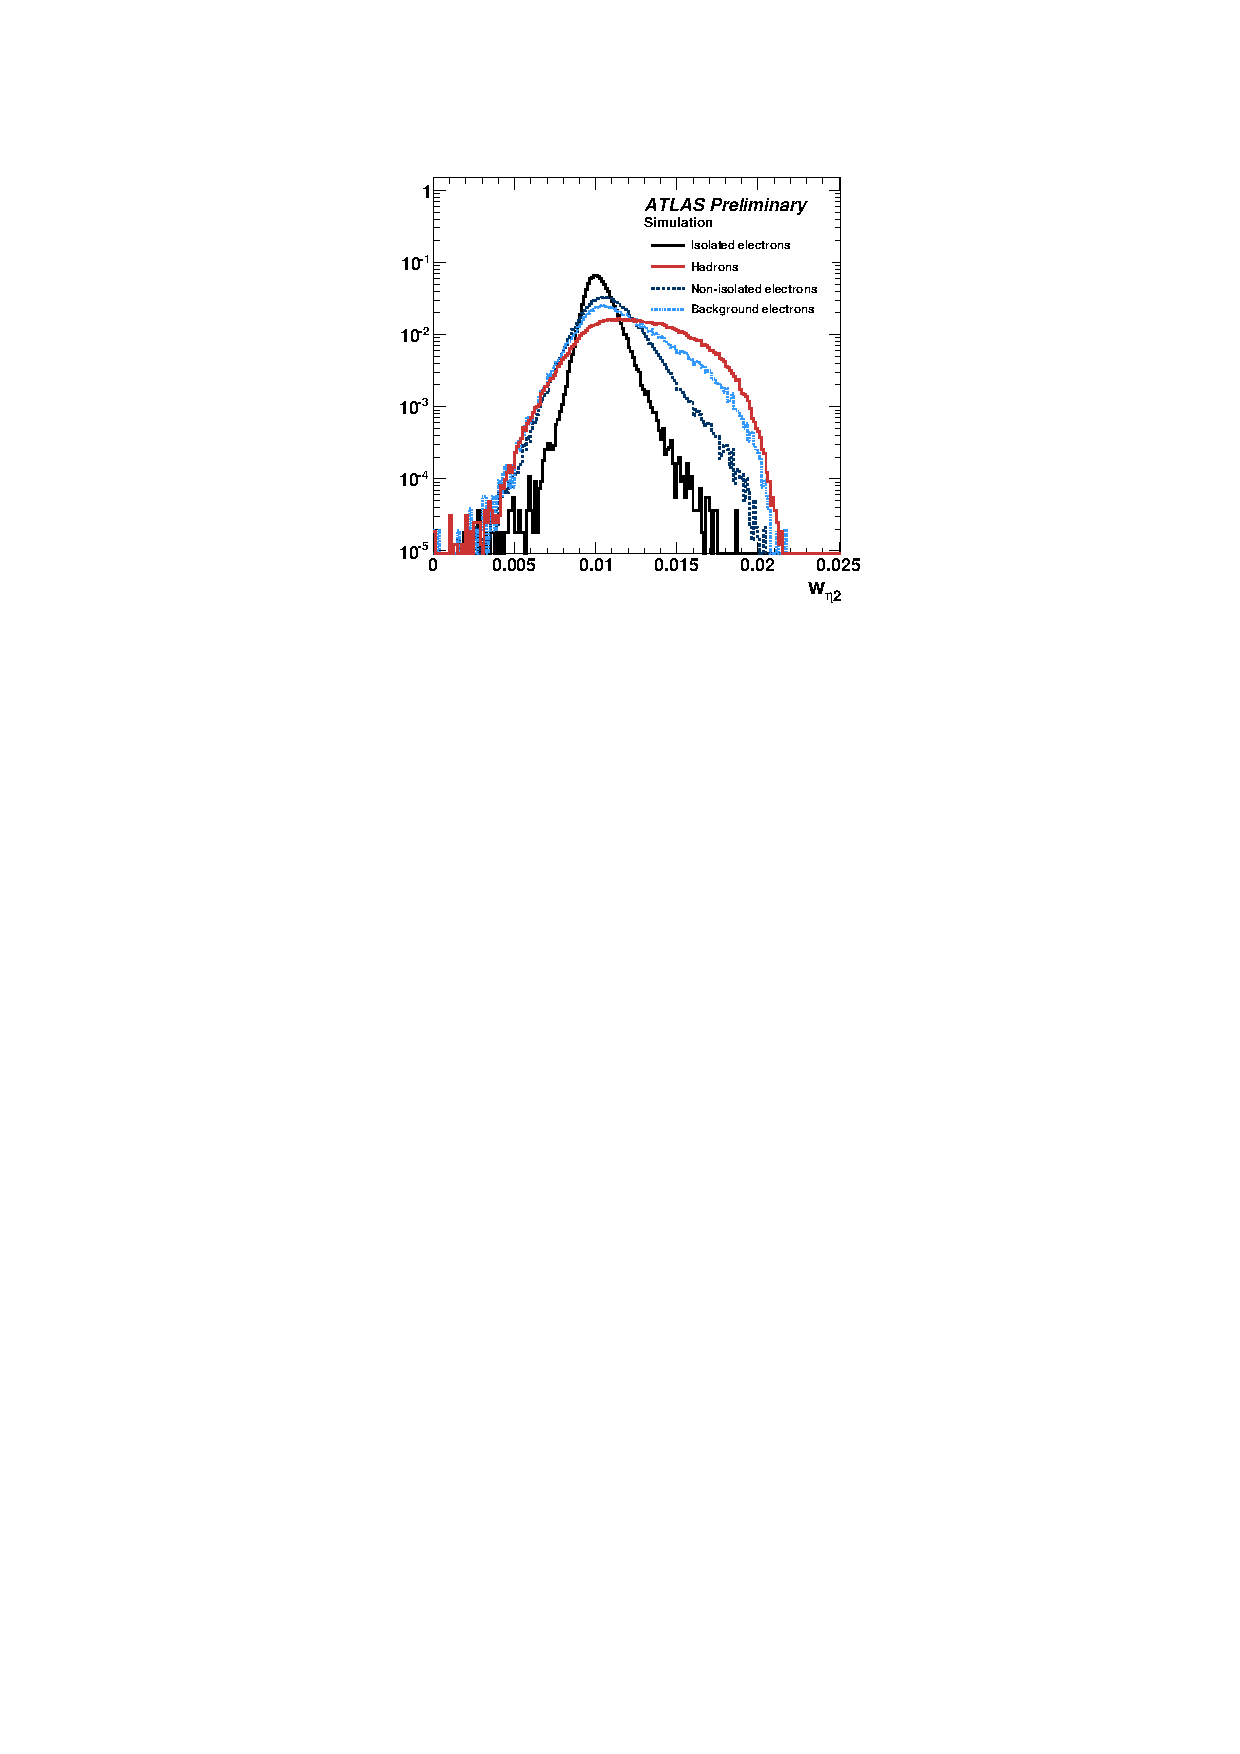
\includegraphics[width=0.2\textwidth]{imagens/egamma_padrao/egamma_padrao_weta2.pdf}
        }
        \subfigure[\protect\acrshort{reta}.]{%
            \label{fig:reta}
            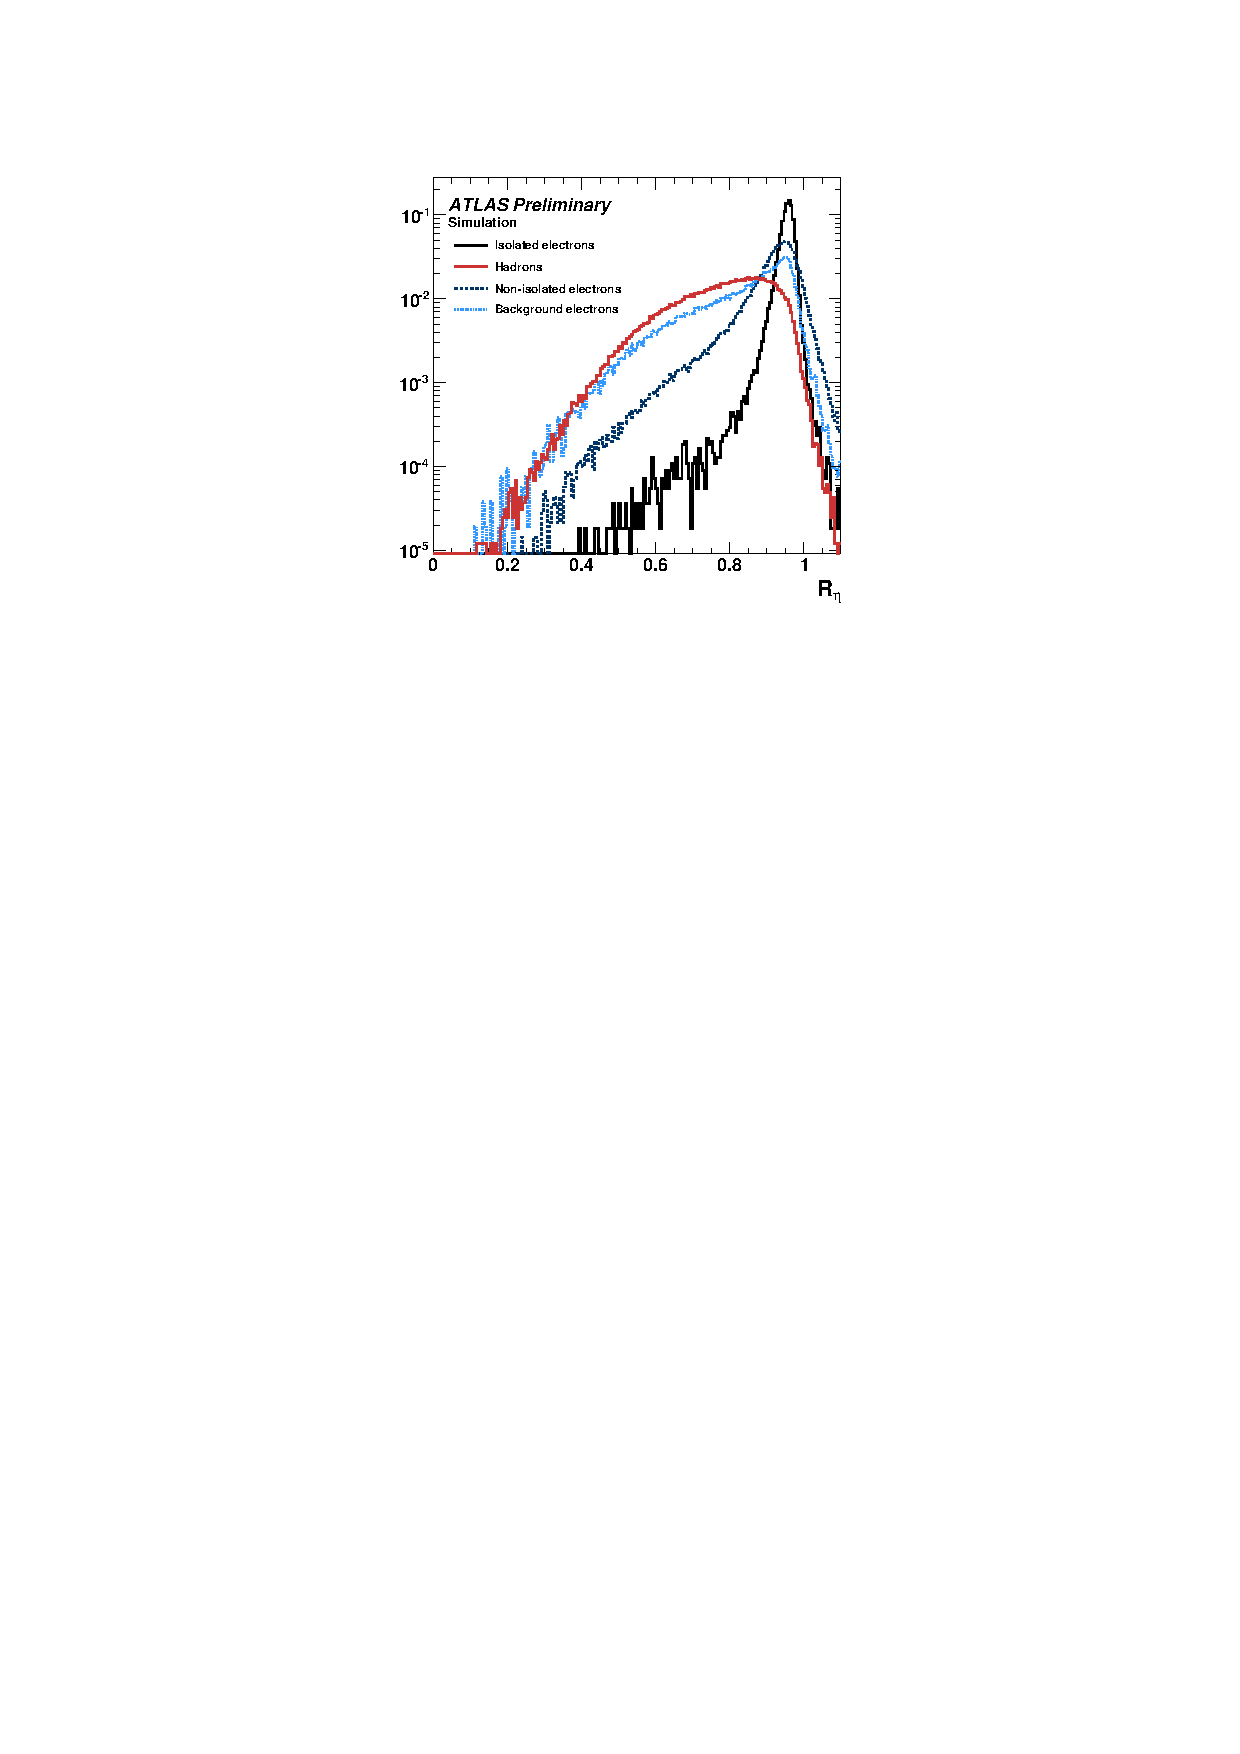
\includegraphics[width=0.2\textwidth]{imagens/egamma_padrao/egamma_padrao_reta.pdf}
        }
        \subfigure[\protect\acrshort{wstot}.]{%
            \label{fig:wstot}
            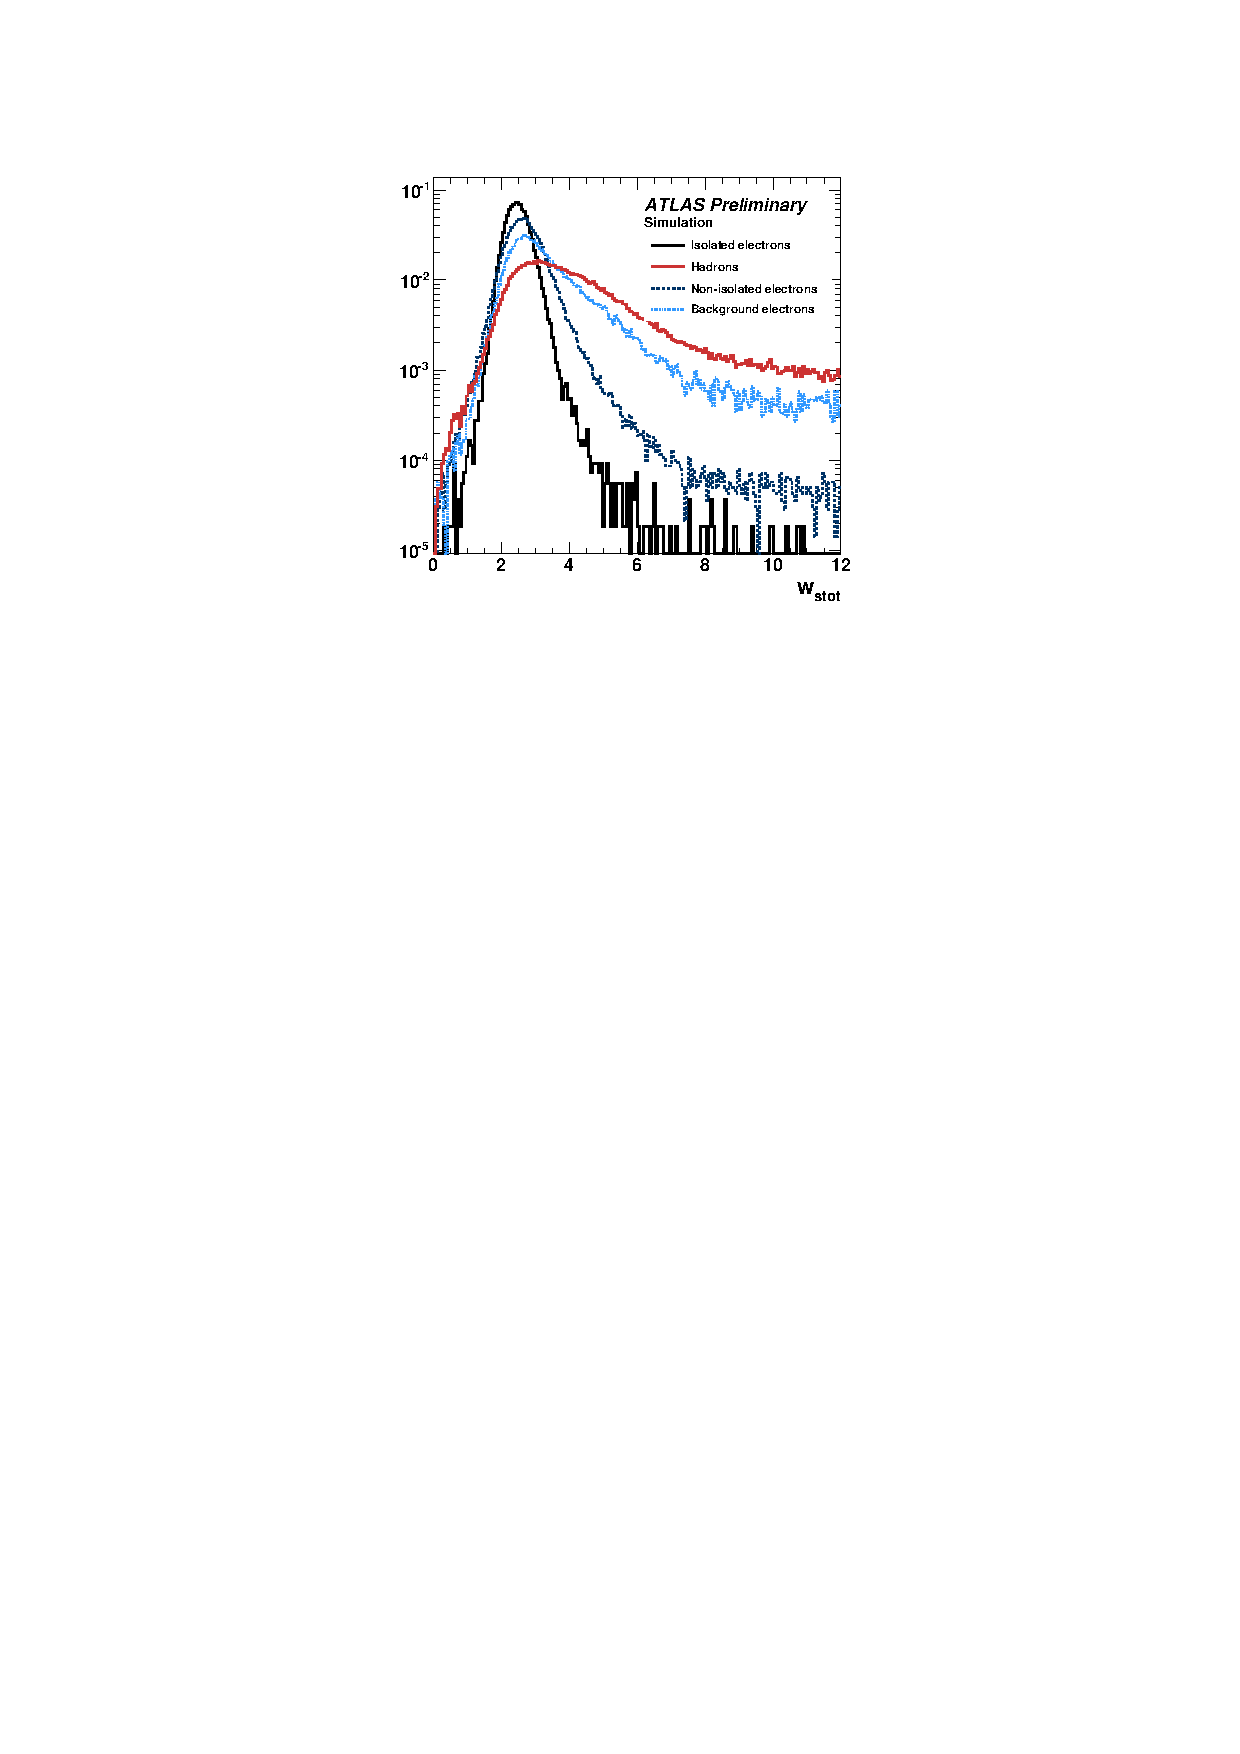
\includegraphics[width=0.2\textwidth]{imagens/egamma_padrao/egamma_padrao_wstot.pdf}
        }\\
        \subfigure[\protect\acrshort{eratio}.]{%
            \label{fig:eratio}
            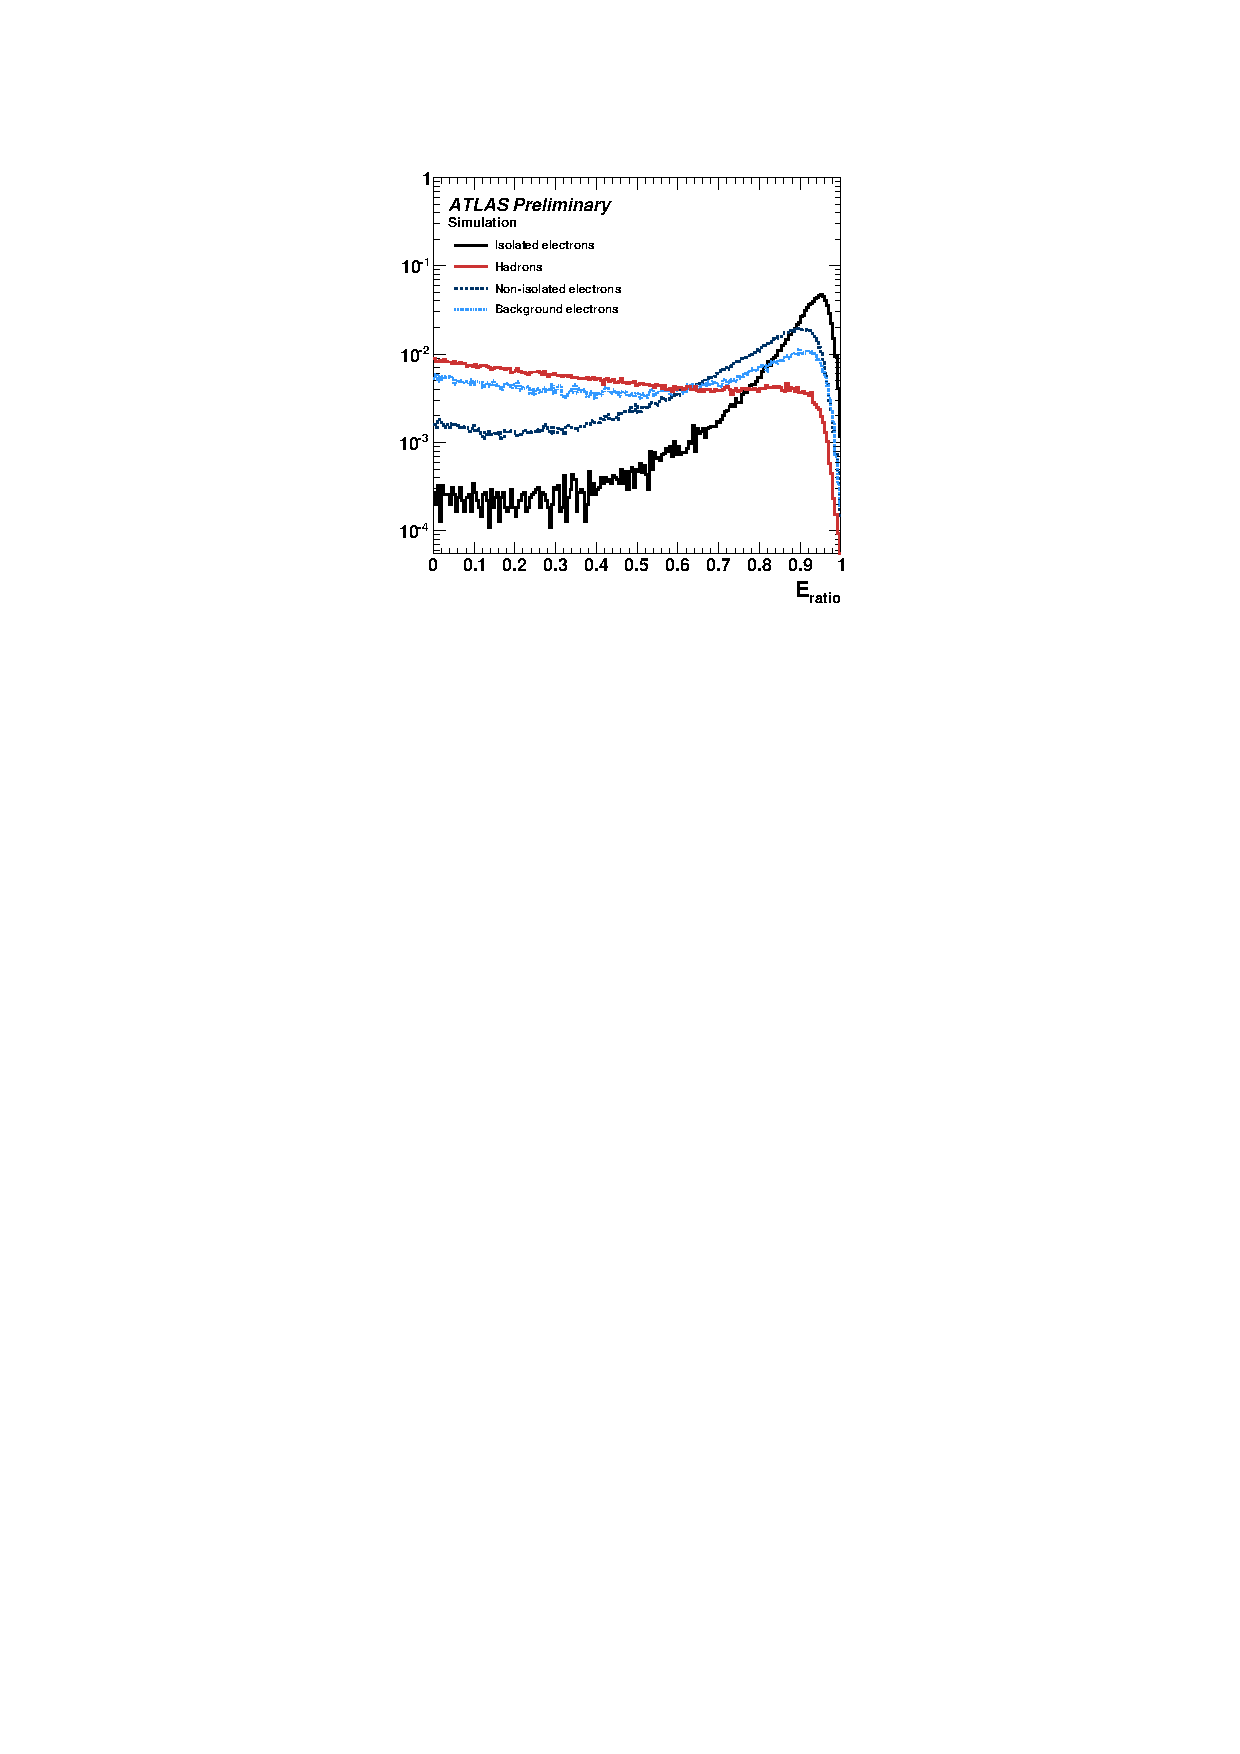
\includegraphics[width=0.2\textwidth]{imagens/egamma_padrao/egamma_padrao_eratio.pdf}
        }
        \subfigure[\protect\acrshort{d0}.]{%
            \label{fig:d0}
            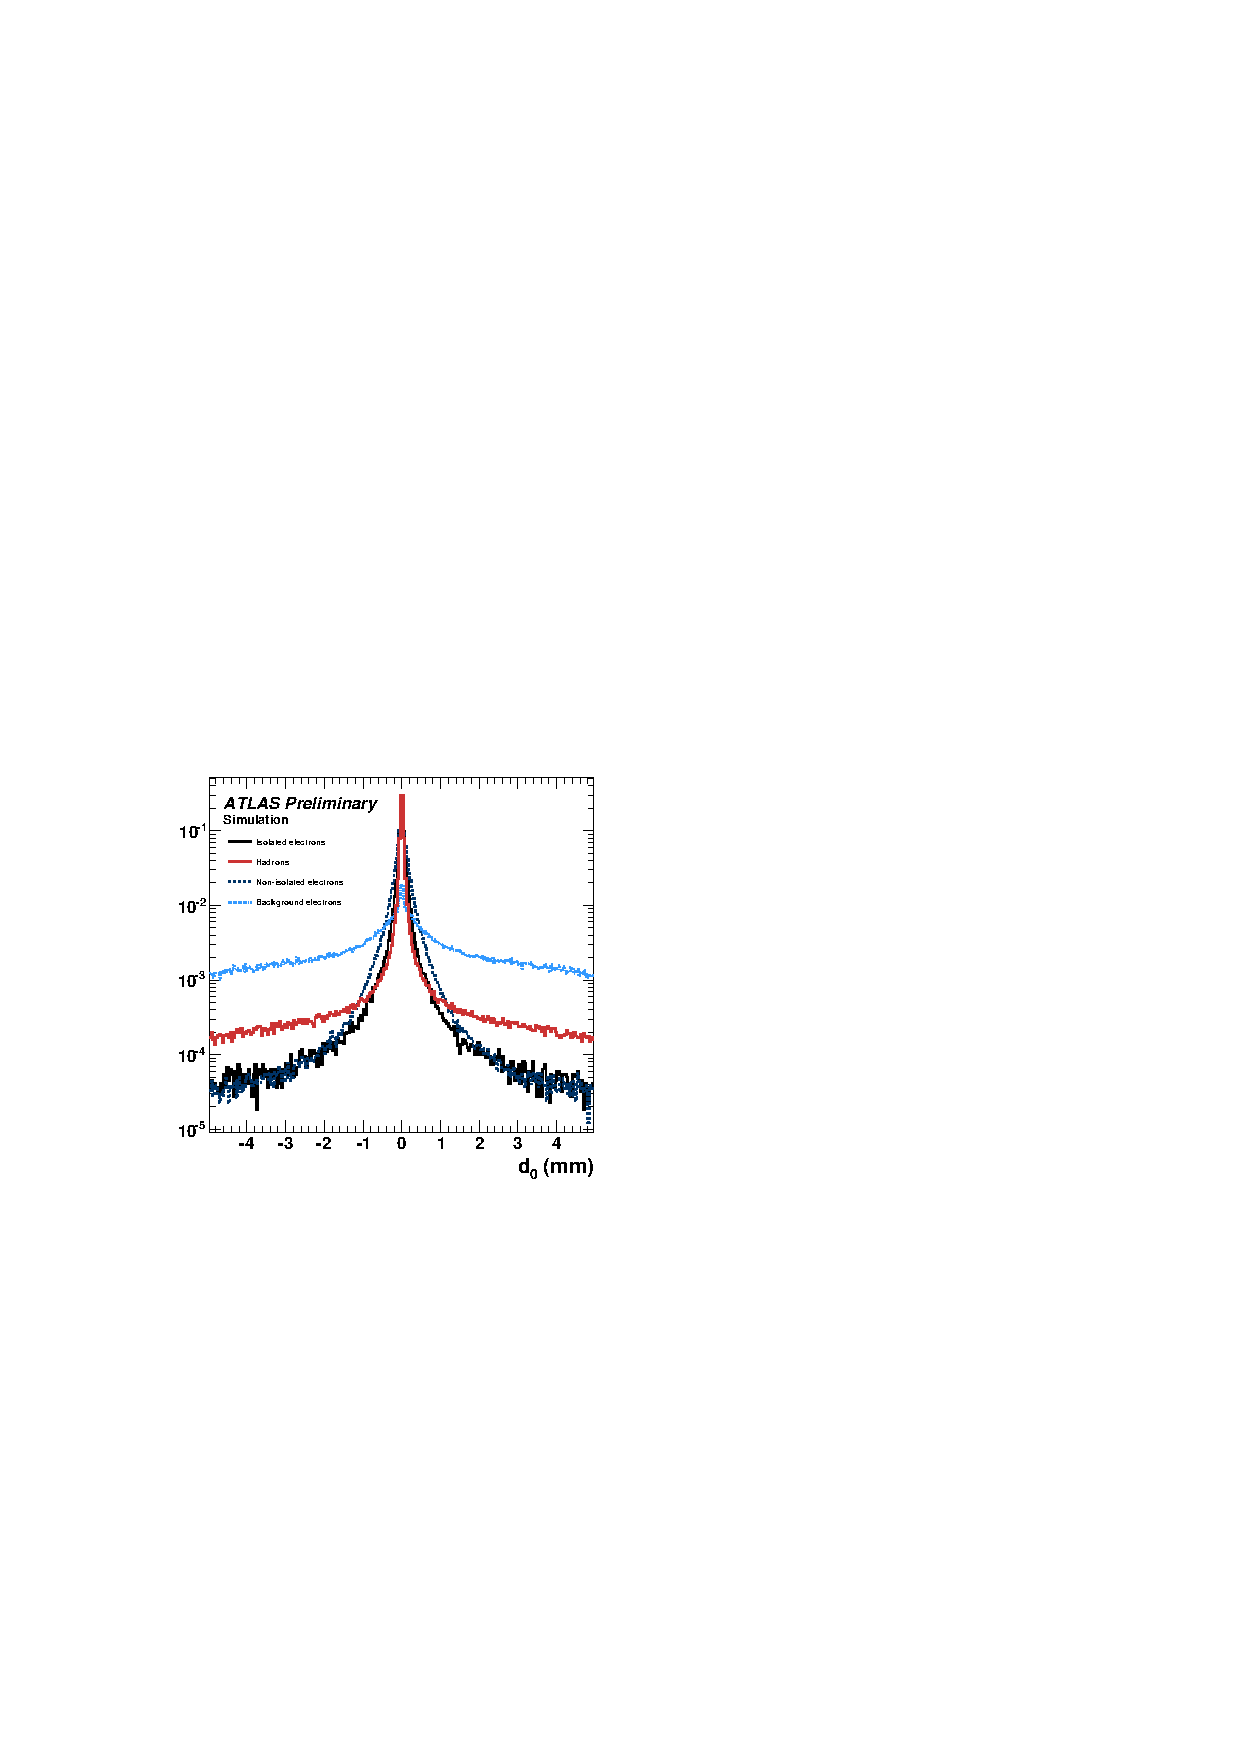
\includegraphics[width=0.2\textwidth]{imagens/egamma_padrao/egamma_padrao_d0.pdf}
        }
        \subfigure[\protect\acrshort{deta1}.]{%
            \label{fig:deta1}
            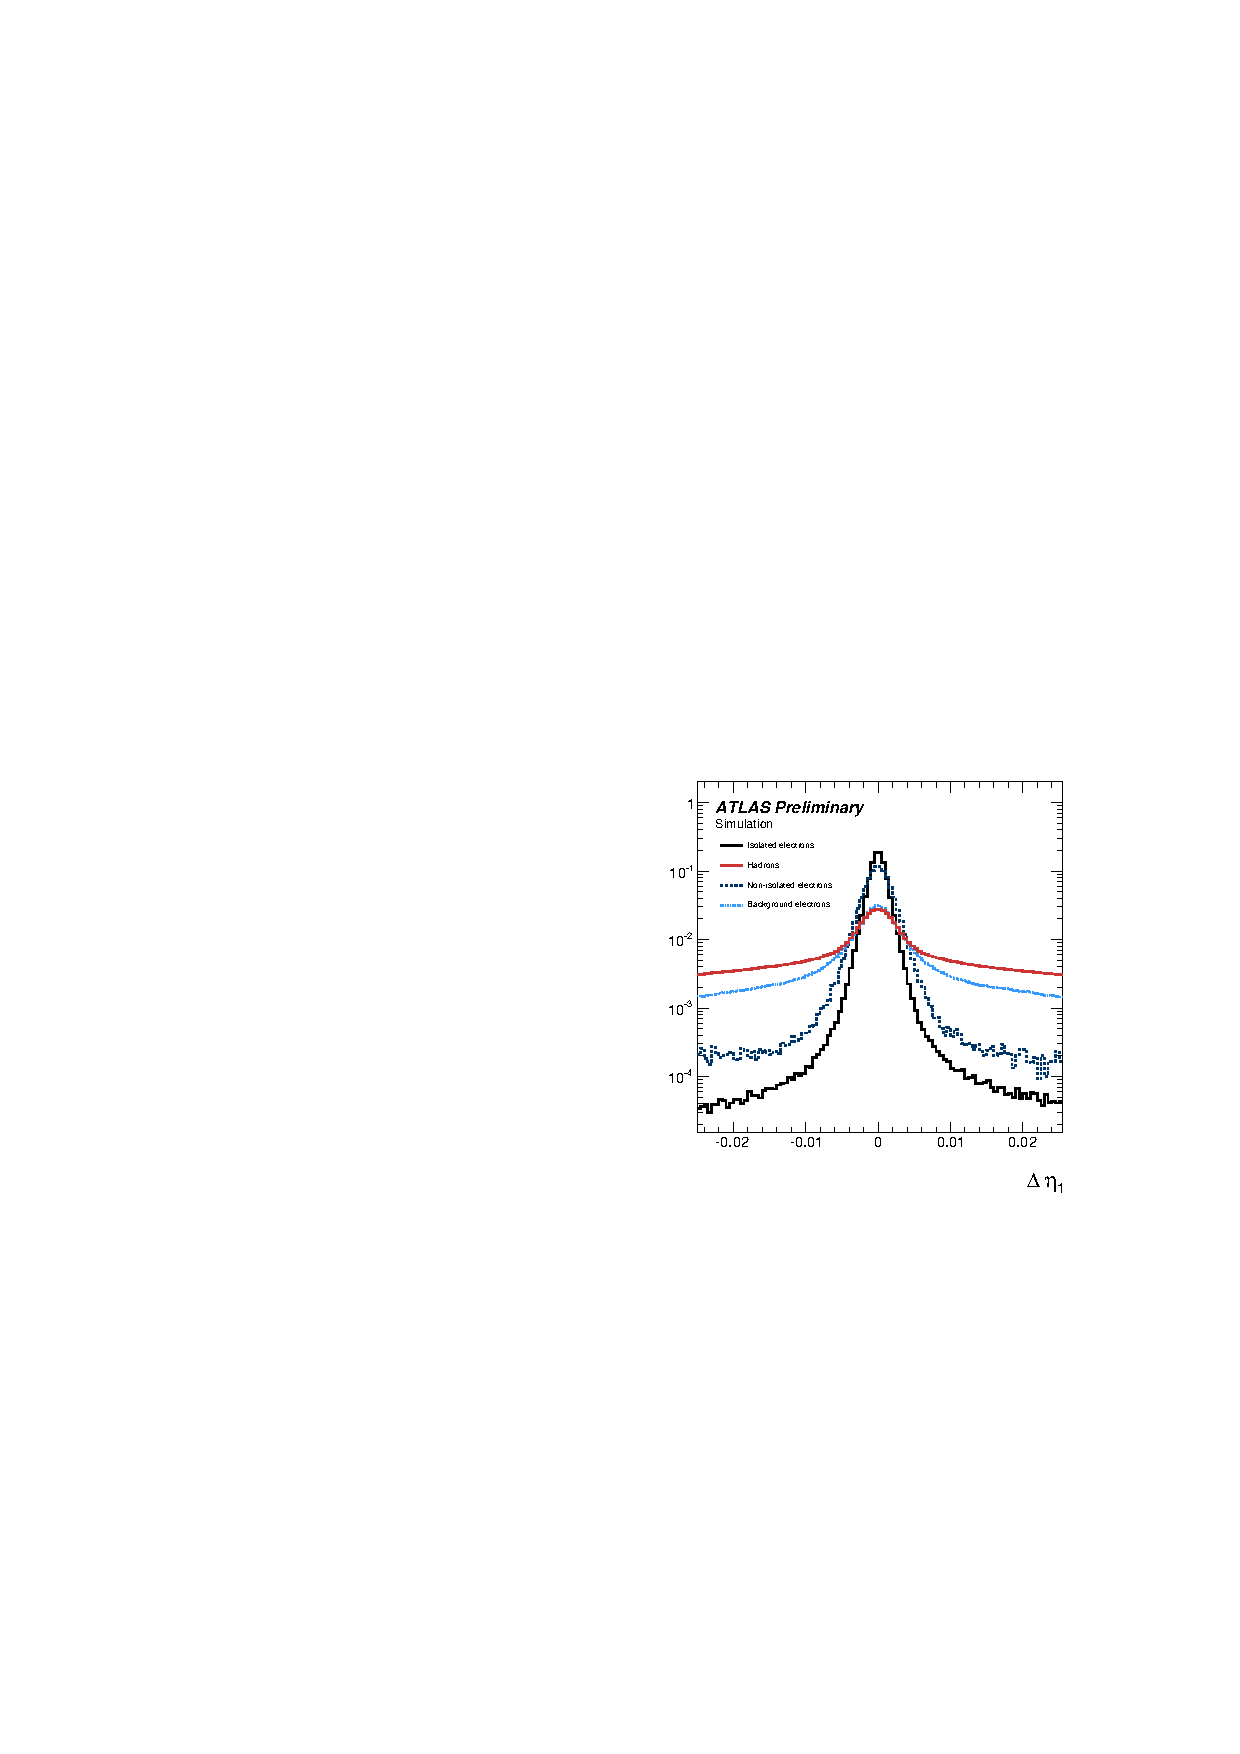
\includegraphics[width=0.2\textwidth]{imagens/egamma_padrao/egamma_padrao_deltaeta1.pdf}
        }
        \subfigure[\protect\acrshort{Ep}.]{%
            \label{fig:Ep}
            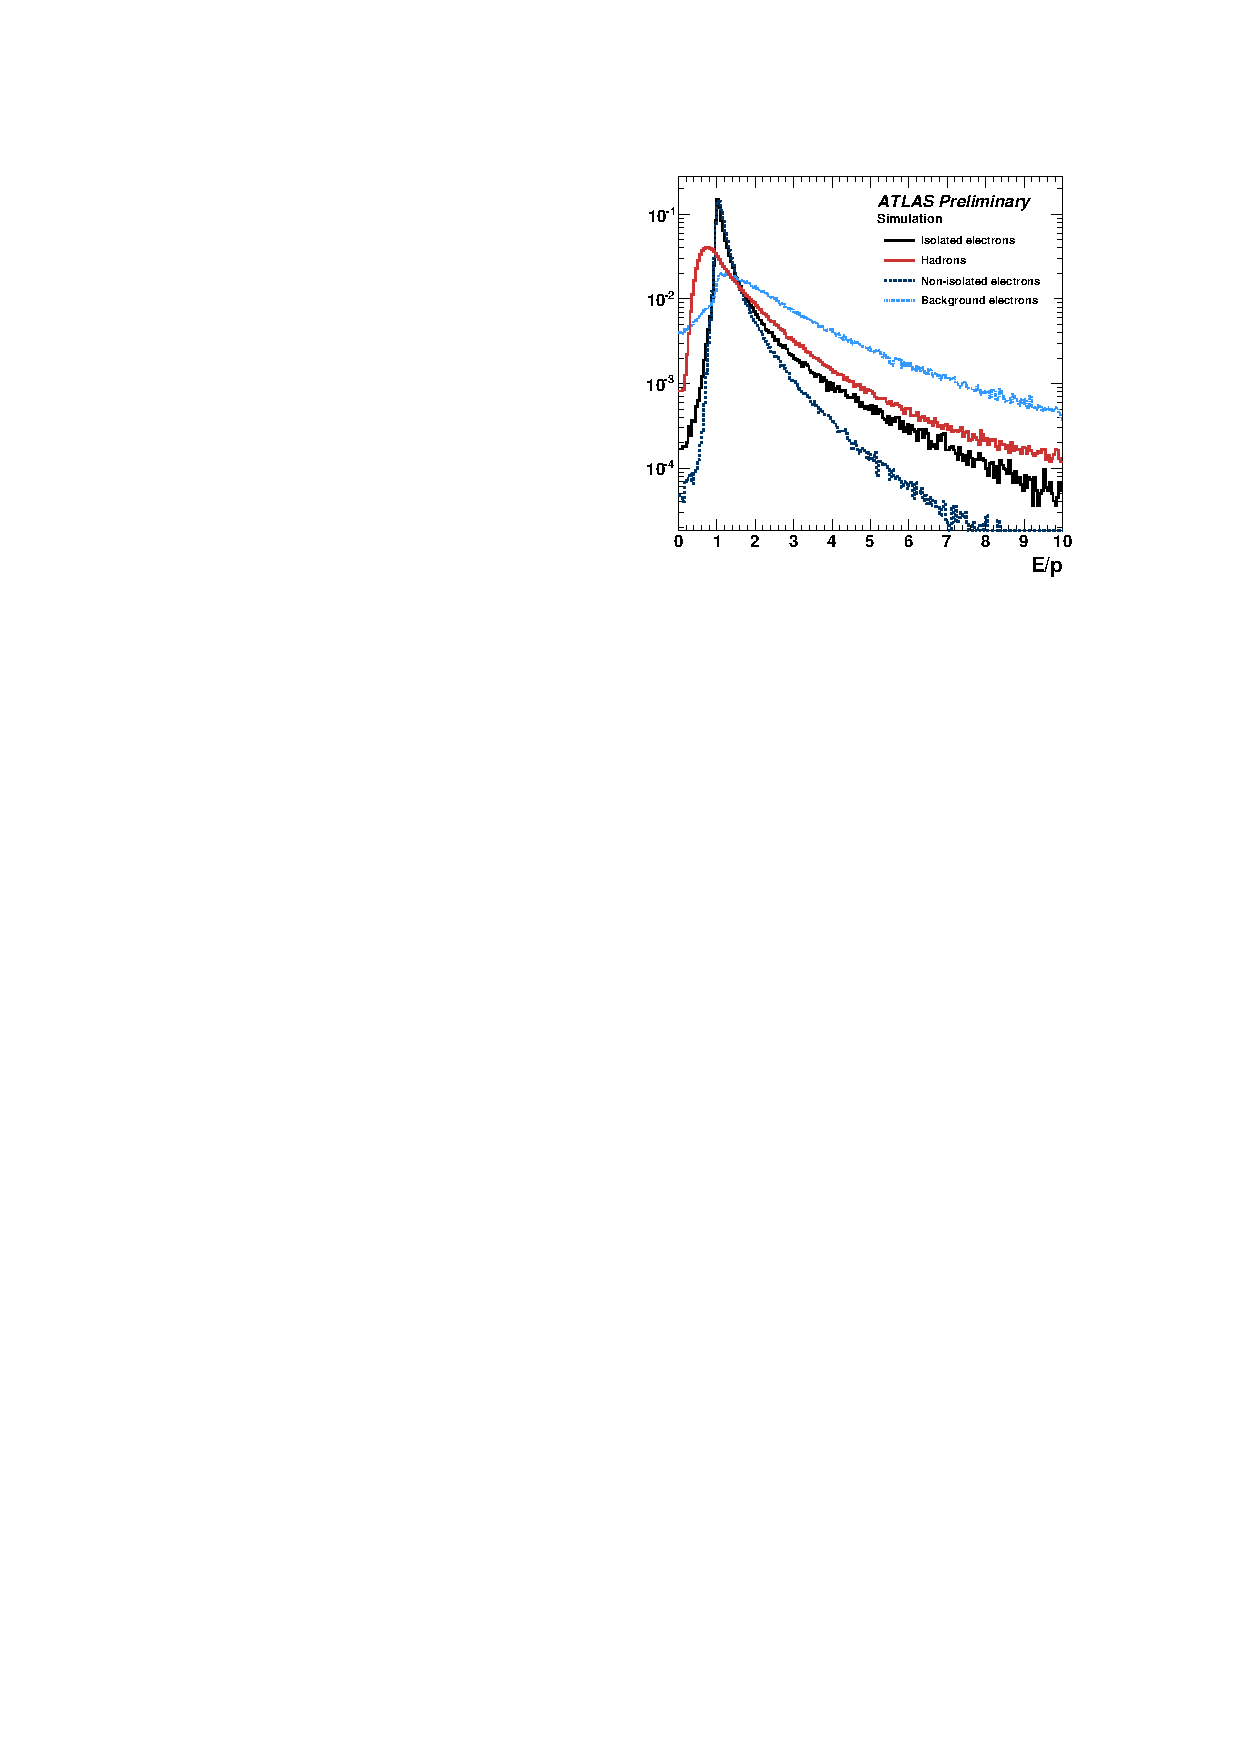
\includegraphics[width=0.2\textwidth]{imagens/egamma_padrao/egamma_padrao_ep.pdf}
        }
\caption[Distribuição de elétrons e seu ruído físico para algumas das variáveis
dos algoritmos e/$\gamma$ padrões.]
{Distribuição de elétrons e seu ruído físico para algumas das variáveis
dos algoritmos e/$\gamma$ padrões. Em preto, elétrons isolados; em vermelho,
hádrons; em azul escuro pontilhado, elétrons não-isolados; e em azul claro
pontilhado, elétrons constituintes de ruído. Extraído de \cite{expected_perf_2011}.}
\label{fig:cortes_egamma_padrao}
\end{sidewaysfigure}

É possível observar os diferentes comportamentos para cada uma das
categorias. Por exemplo, elétrons isolados na variável \gls{reta},
Figura~\ref{fig:reta}, possuem grande parte de valores próximos a 1, 
uma vez praticamente toda sua energia estará depositada no centro da 
\gls{roi}, por outro lado, hádrons distribuem sua energia em um espaço maior da
\gls{roi}, de forma que ao realizar a fração \gls{reta}, obterá-se geralmente
valores menores de 1. No caso da variável
\gls{eratio}, \ref{fig:eratio}, é esperado o mesmo valor para elétrons isolados,
onde a diferença de deposito entre as duas células de maior
energia deverá ser grande para elétrons, uma vez que os mesmos terão grande parte 
de sua energia depositada na célula de maior energia, e pequeno para os hádrons. Cada variável
tem sua distribuição especifica, mas reflete uma diferença física da interação
de hádrons e elétrons com o detector.


\subsection{HLT\_EgammaCaloRinger (HLT\_Ringer)}
\label{ssec:hlt_ringer}

\newacronym[type=Abrev,\glslongpluralkey={Redes Neurais Artificiais}]
{rna}{RNA}{Rede Neural Artificial}
\newacronym[type=Abrev]{ica}{ICA}{Análise de Componentes Independentes}
\newacronym[type=Abrev]{nlica}{NLICA}{Análise de Componentes Independentes
Não-Linear}
\newacronym[type=Abrev]{pca}{PCA}{Análise de Componentes Principais}
\newacronym[type=Abrev]{pcd}{PCD}{Componentes Principáis de Discriminação}
\newacronym[type=Abrev]{som}{SOM}{Mapas Auto-Organizáveis}

Uma outra proposta para se identificar a evolução do chuveiro no calorímetro é 
abordada pelo algoritmo alternativo proposto, afim de se identificar as
partículas \gls{em}. Como o algoritmo é proposto para atuar sobre as variáveis
do calorímetro, ele não faz distinção de elétron e pósitrons para fótons, essa
distinção pode ser realizada posteriormente utilizando a informação do \gls{id}.
Inicialmente esse algoritmo, chamado de \gls{hltringer}, foi planejado para operar no
\acrlong{l2} como uma alternativa ao \gls{t2calo}, o ambiente mais restritivo 
em questões de tempo. Ao invés de gerar diversas variáveis de interpretação física 
para a compreensão da interação da partícula com o calorímetro, como os já
citados: \gls{eratio}, \gls{reta} e \gls{Rhad1}; o algoritmo utiliza a informação anelada
de calorimetria como o seu \gls{fex} (Tópico~\ref{sssec:anelamento}) 
e um processo de discriminação para o seu \gls{hypo}. Qualquer método estatístico 
pode ser aplicado para realizar o processo de discriminação. 
Em partícular, os estudos deste trabalho utilizaram \glspl{rna} \cite{neural_networks} 
(Tópico~\ref{sssec:rna}), pois obtiveram melhor perfomance nos estudos
realizados no inicio do projeto.

Diversas técnicas de pré-processamento podem ser combinadas com redes neurais de
forma a melhorar a sua eficiência de discriminação. Estudos anteriores
\cite{tese_eduardo,tese_torres} utilizaram métodos como \gls{ica}, \gls{pca},
\gls{nlica}, \gls{som} e \gls{pcd}, obtendo resultados melhores que uma
abordagem utilizando diretamente \gls{rna}. Um caso especial de pré-processamento 
de dados, necessaria quando utilizando redes neurais, é a normalização dos dados. Esse 
pré-processamento ajusta o alcânce de energia dos anéis ao alcânce dinâmico das
\gls{rna}. Uma grande gama de métodos de normalização são utilizados, podendo
gerar alterações no espaço de representação de anéis, de forma que a
interpretação da nova representação pode ter uma melhor, ou pior, interpretação
pela \gls{rna}. As normalizações testadas para otimizar a eficiência do
\gls{hltringer} estão explicadas no Tópico~\ref{sssec:preproc_norm}.

\subsubsection{O processo de anelamento}
\label{sssec:anelamento}

\begin{figure}[hp!]
\label{fig:cons_aneis}
\centering
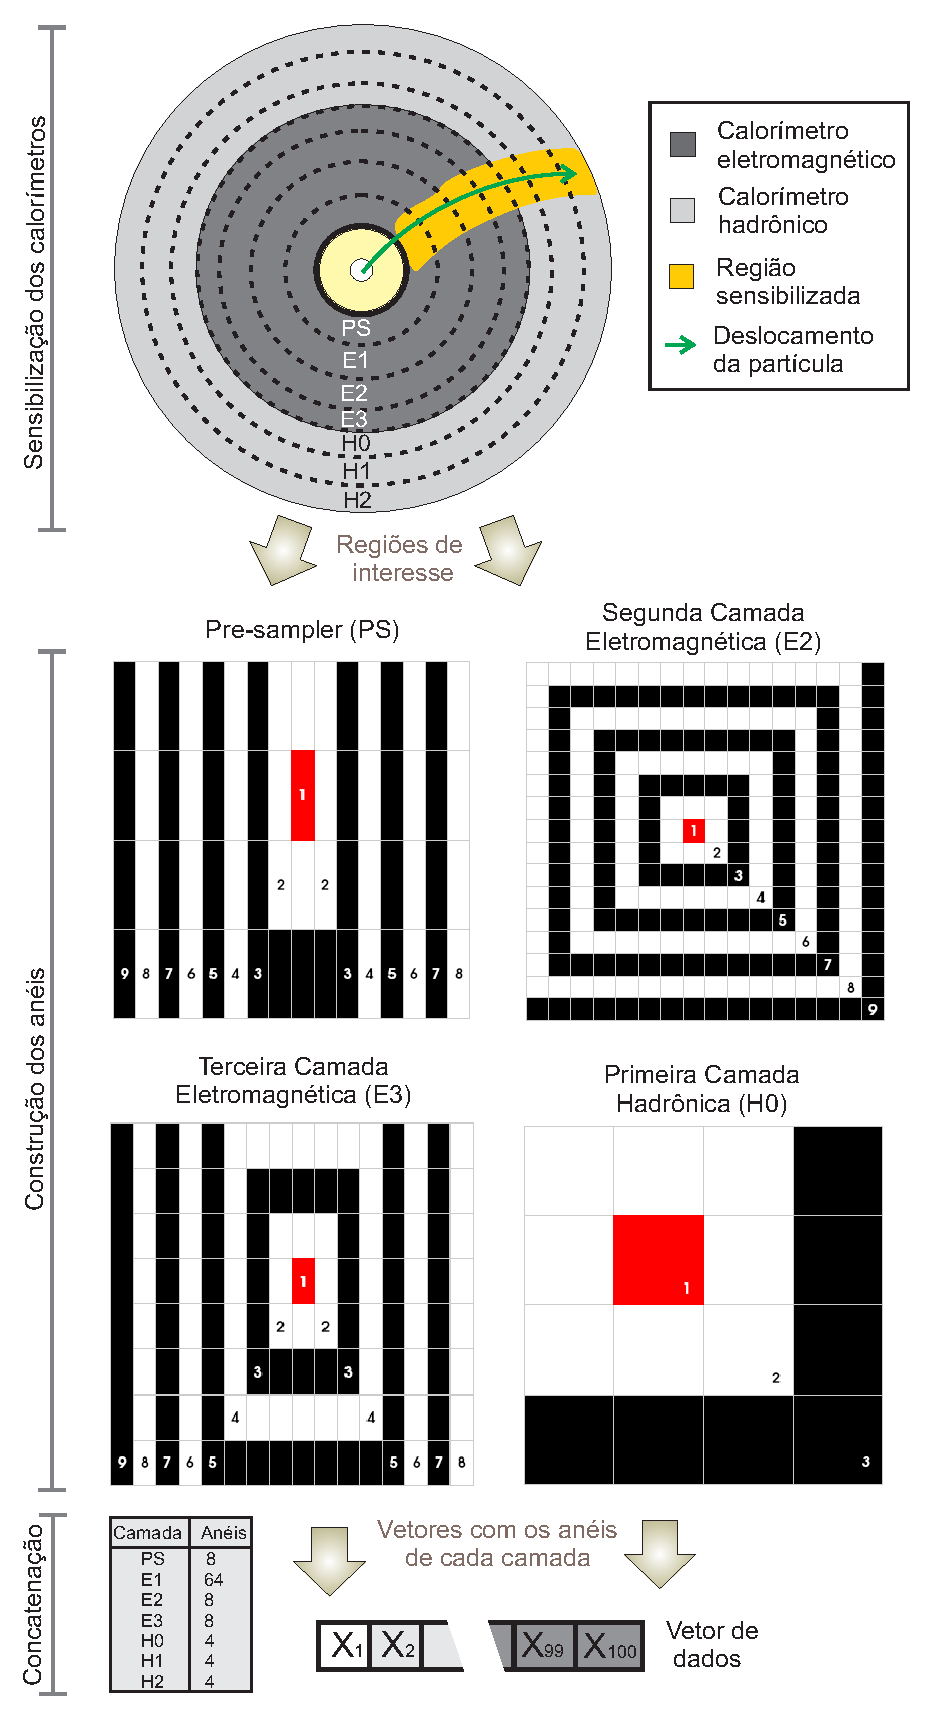
\includegraphics[height=0.9\textheight]{imagens/cons_aneis.pdf}
\caption[Diagrama do processo de construção dos anéis.]
{Diagrama do processo de construção dos anéis. Extraído de \cite{tese_eduardo}.}
\end{figure}

O processo de anelamento, esboçado na Figura~\ref{fig:cons_aneis}, é realizado
para todas as camadas (\gls{ps}, \gls{e1}, \gls{e2}, \gls{e3}, \gls{h0},
\gls{h1} e \gls{h2}) do Sistema de Calorimetria do \gls{atlas}. Como foi dito,
no \gls{l2} a semente utilizada para a construção do aglomerado é a célula quente  -- ou a célula mais
energética -- da \gls{e2} na \gls{roi} gerada a partir da posição 
fornecida pelo \gls{l1}. No \gls{hltringer}, ao invés da construção do
aglomerado, é realizada a construção de anéis concêntricos, onde essa célula
será o núcleo, e sua energia a informação contida no primeiro anel, o anel central. 
Os anéis posteriores contêm a soma da energia das células adjacentes
exteriores ao anel anterior, por exemplo, no caso do segundo anel, as células imediatamente
exteriores a célula quente. Esse processo irá se repetir até que uma região pré-determinada seja
completamente preenchida. Atualmente o valor utilizado é de $0,4\times0,4$ em
$\Delta\eta\times\Delta\phi$. Nas outras camadas, a posição da
semente é utilizada para encontrar a célula central e o processo é repetido, até
que a mesma região seja preenchida, entretanto, como a granularidade das células
do calorímetro variam conforme a segmentação longitudinal, o número de anéis variam
para cada camada. O conceito de anéis é abstrato: como o \gls{l2} calcula
um novo centro na \gls{roi} formada a partir da informação fornecida pelo
\gls{l1}, anéis podem por ventura necessitar de células exteriores a \gls{roi},
e essas, não estando disponíveis para o \gls{l2}, geram anéis incompletos,
como aqueles ilustrados para o \gls{ps} a partir do terceiro anel. 
No caso de nenhuma célula estiver disponível para um dado anel, é então atribuido valor
nulo ao mesmo para garantir que o processo complete o número necessário no
preenchimento da região. Os anéis esboçados na figura são meramente
ilustrativos, não possuindo a proporção real para cada uma das camadas, nem o
número de anéis totais para cada uma delas. Um total de 100 anéis foram 
especificados inicialmente, divididos conforme as camadas da maneira indicada na
tabela contida no final dessa figura. Note que a quantidade de anéis é proporcional 
a granularidade de cada camada. Em uma discriminação não-segmentada
(veja~\ref{sssec:rna}), os anéis são contenados em um grande vetor de dados,
como indicado.

O processo de anelamento reduz a quantidade de informação a ser analisada no
calorímetro, ao se agrupar diversas células em uma única informação, reduzindo
as $\sim$1000 células dentro da \gls{roi} em 100 anéis, ou seja, um fator de
compactação de $\sim$10$\times$. Indo além, o número total de anéis a serem
propagados para o método de discriminação pode ser reduzido através de estudo
com quantidade elevada de estatística do processo. Entretanto, a redução de informação 
é utilizada para se referir a compactação da
informação das células do calorímetro nos anéis, não podendo se comparar 
com a ordem de informação armazenada nas variáveis físicas, 
que se resumem a cerca de 5 variáveis.

Ao mesmo tempo, a interpretação física da propagação do
chuveiro é mantida, como a sua espessura lateral e profundidade longitudinal. 
Na Figura~\ref{fig:perfil_aneis} está um 
exemplo da deposição de energia de elétrons e de um dos hadrôns que
compõem os jatos hadrônicos\footnote{Para evitar a repetição, quando se
referindo a jatos no Canal \gls{eg}, estará se mencionando os hádrons individuais
que formam os jatos hadrônicos, e não o conjunto. O canal de reconstrução de
jatos, diferente do Canal \gls{eg}, reconstrói o jato como um todo, 
o que pode gerar confusão na nomenclatura.} para a \gls{e2}. Pode-se observar na parte
superior da figura a deposição de energia nas células do calorímetro, onde os
jatos possuem um perfil de deposição mais largo, como o esperado para o chuveiro
dessas partículas, quando em comparação com a deposição de energia de um
elétron. Este, por sua vez, tem sua deposição de energia concentrada no centro da
\gls{roi}. A parte inferior, contendo a deposição de energia nos anéis formados 
para cada um dos caso, demonstra a diferença de ambos, onde elétrons depositam grande parte de
sua energia no primeiro anel, e pouca energia nos anéis mais externos, enquanto
os jatos possuem um perfil mais disperso, alcançando anéis mais externos.

\begin{figure}[ht!]
\label{fig:perfil_segunda_camada}
\centering
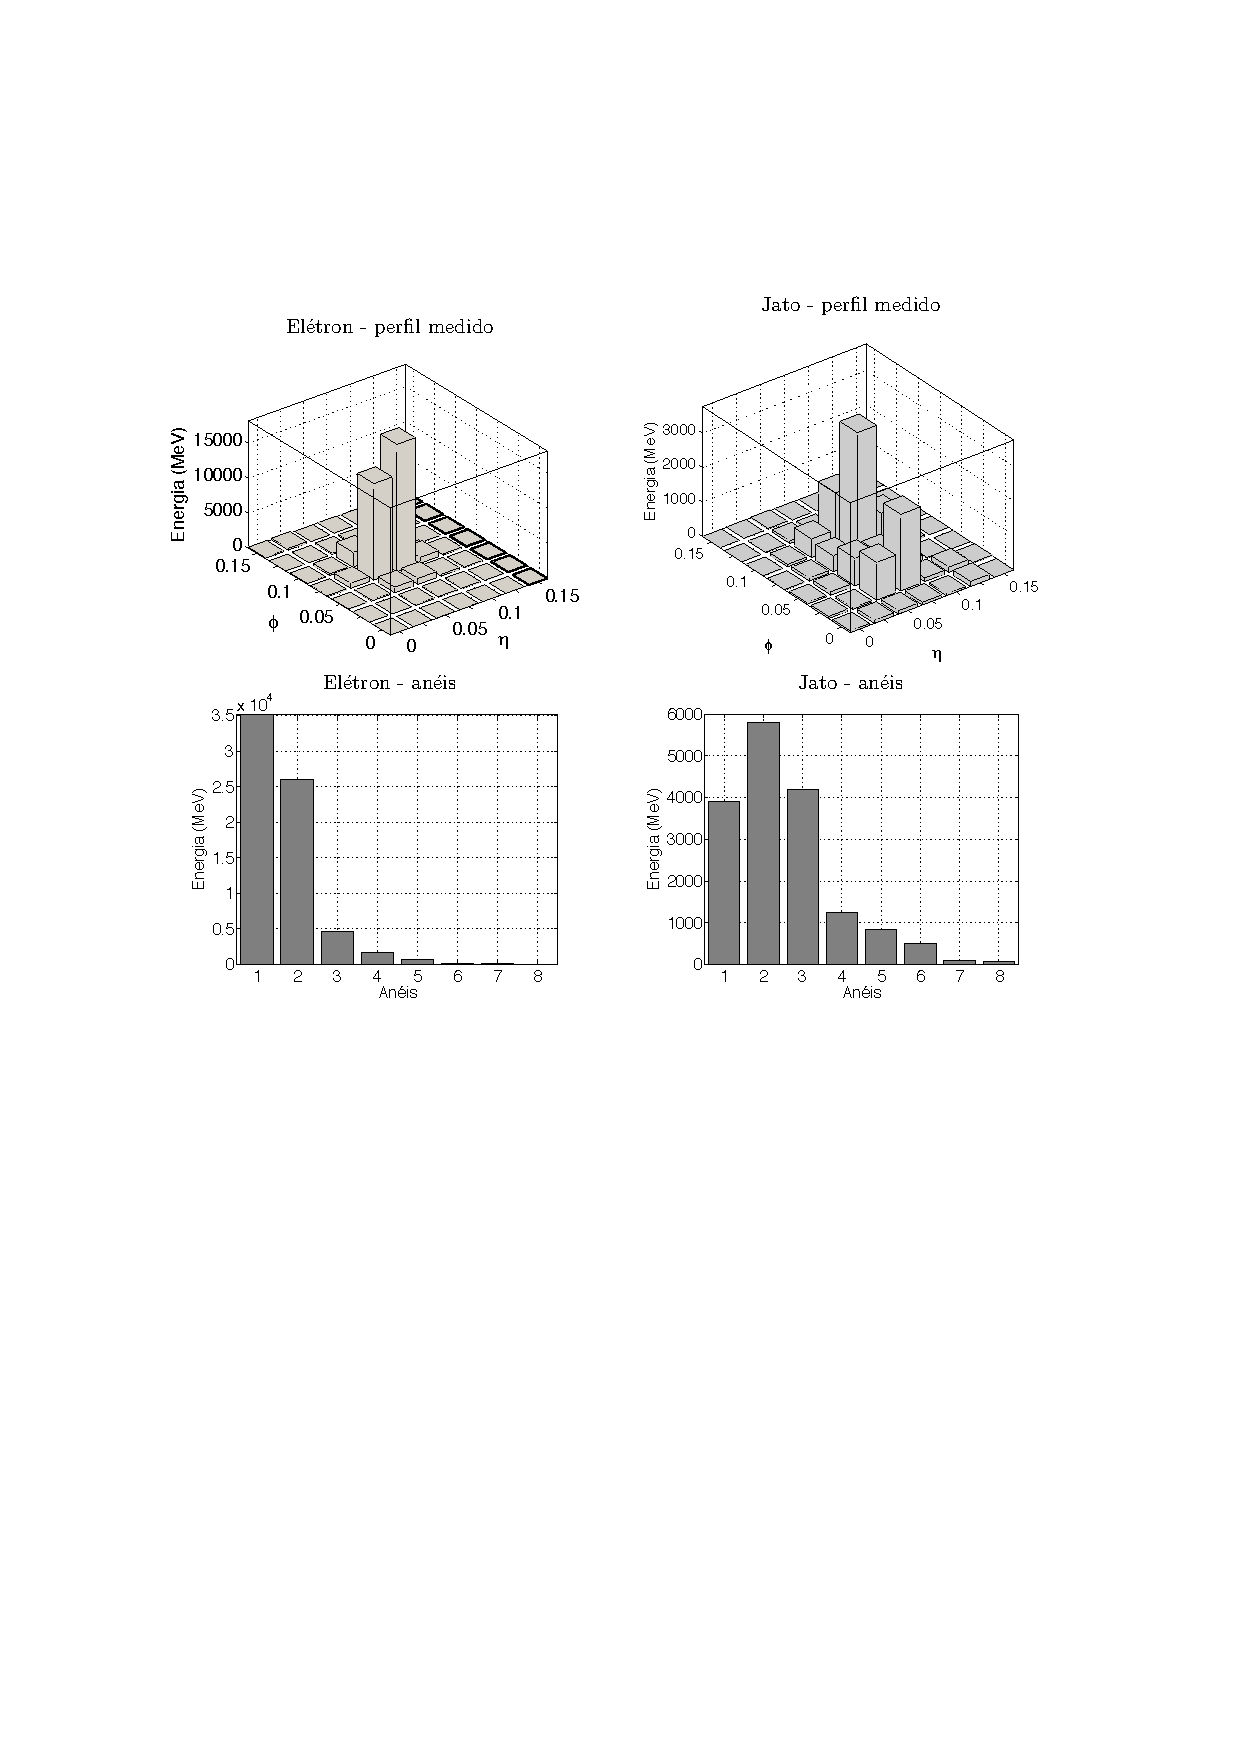
\includegraphics[width=0.9\textwidth]{imagens/segunda_camada_celulas.pdf}
\caption[Perfil de distribuição de energia nas células e anéis na segunda camada para 
elétrons e jatos.]{Perfil de distribuição de energia nas células e anéis na segunda camada 
para elétrons e jatos. Extraído de \cite{tese_eduardo}.}
\end{figure}

Quando considerando a distribuição de energia em anéis de uma maneira global,
pode-se observar a diferença dos perfis dos chuveiros \gls{em} e
\gls{had}. A Figura~\ref{fig:perfil_aneis} contêm o perfil dos 100 anéis para um
elétron (\ref{fig:perfil_aneis_eletron}) e um jato
(\ref{fig:perfil_aneis_jato}), onde a distribuição citada para elétrons e jatos
na \gls{e2} se repete para as outras camadas do \gls{ecal}, com os jatos
distribuindo sua energia nos anéis mais externos. Por outro lado, os elétrons
geralmente não alcançam as camadas hadrônicas, sendo absorvidos pela
\gls{e2} ou \gls{e3}, enquanto jatos ultrapassam o \gls{ecal} depositando
energia no \gls{hcal}. Contudo, esse fato nem sempre é verdadeiro, elétrons
muito energéticos podem acabar ultrapassando a \gls{e3} e depositando parte de
sua energia na \gls{h1}, e jatos podem também serem absorvidos no \gls{ecal},
como aquele ilustrado em \ref{fig:perfil_aneis_jato_conf}.

\begin{figure}[ht!]
\label{fig:perfil_aneis}
\centering
  \subfigure[]{%
      \label{fig:perfil_aneis_eletron}
      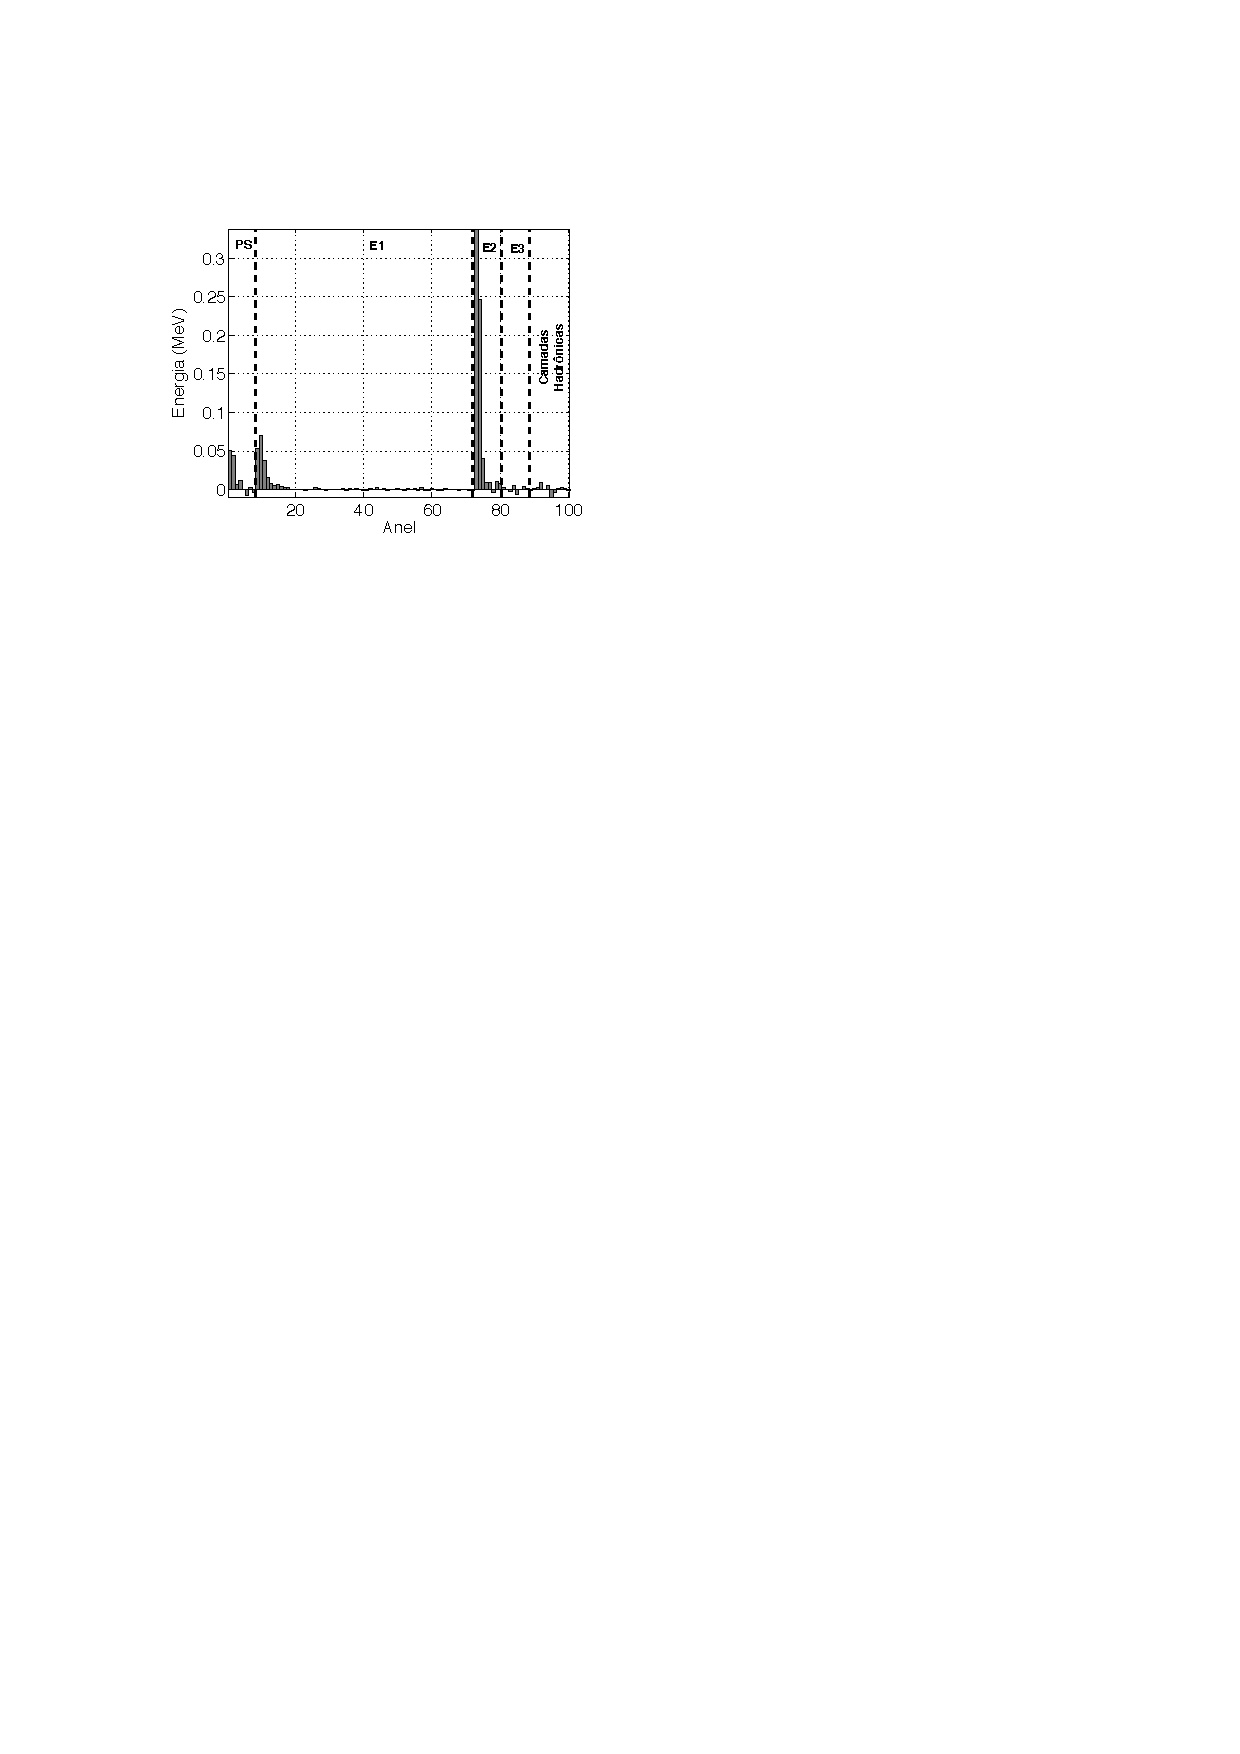
\includegraphics[width=0.45\textwidth]{imagens/perfil_aneis_eletron.pdf}
  }\hspace{0.01\textwidth}
  \subfigure[]{%
      \label{fig:perfil_aneis_jato}
      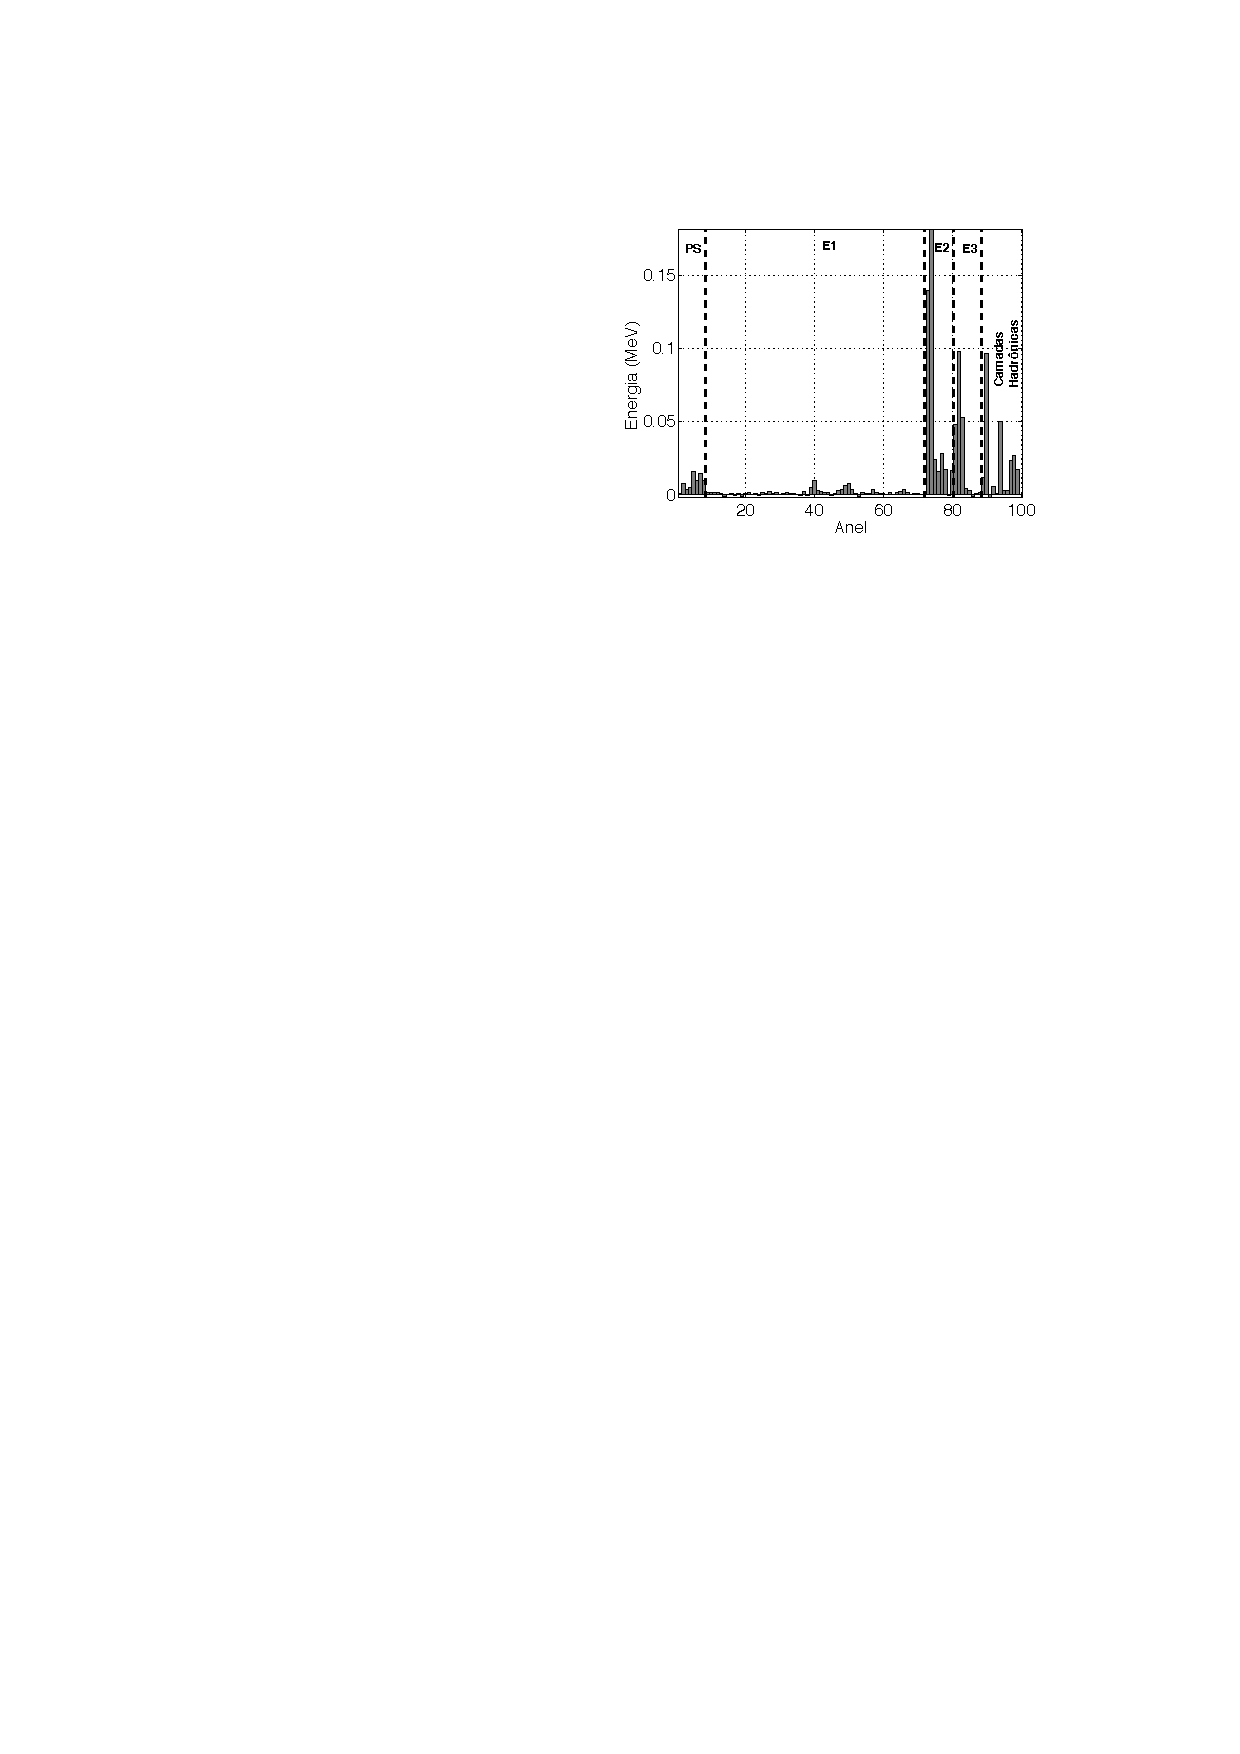
\includegraphics[width=0.45\textwidth]{imagens/perfil_aneis_jato.pdf}
  }\\
  \subfigure[]{%
      \label{fig:perfil_aneis_jato_conf}
      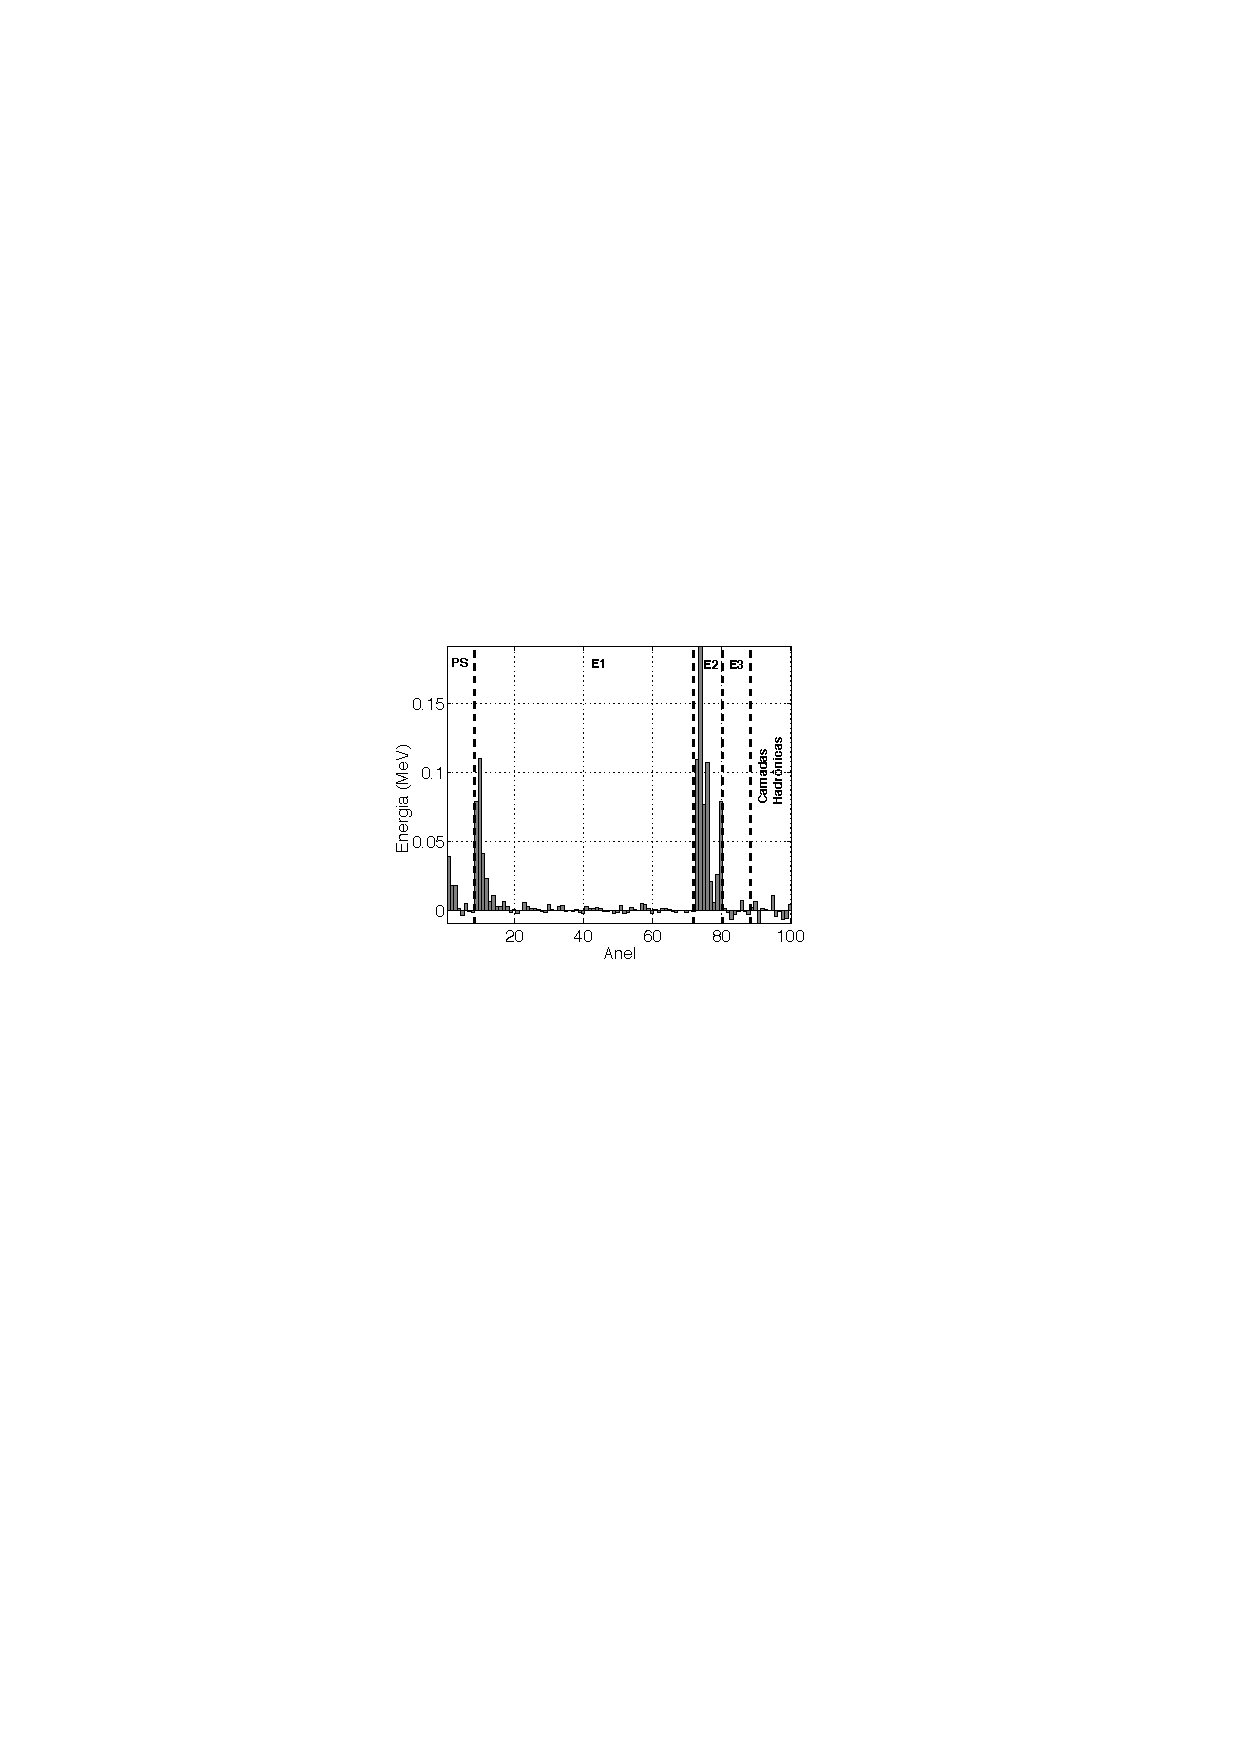
\includegraphics[width=0.45\textwidth]{imagens/perfil_aneis_jato_confundidor.pdf}
  }\\
\caption[Perfil típico para os 100 anéis de elétrons e jatos.]{Perfil típico
para os 100 anéis de elétrons (\ref{fig:perfil_aneis_eletron}) e
jatos (\ref{fig:perfil_aneis_jato}). Jatos atípicos (\ref{fig:perfil_aneis_jato_conf}) 
dificultam o processo de discriminação. A escala de energia está normalizada
pela Norma 1. Extraído de \cite{tese_eduardo}.}
\end{figure}



\subsubsection{Normalização}
\label{sssec:preproc_norm}

Neste tópico estão as descrições das normalizações testadas para a otimização do
\gls{hltringer}. Foram utilizadas normalizações presentes na literatura
utilizando tratamento estatístico dos dados, como a Esferização, MinMax, 
adicionadas de normalizações que fazem mão do conhecimento da topologia dos calorímetros, 
sua segmentação longitudinal e das diferenças entre os chuveiros \gls{em} e \gls{had}, 
buscando realçar suas características, citando entre elas a normalização
sequencial.

\paragraph{Energia Total (Norma 1)}
\label{par:norm_norm1}

Neste modo de normalização, também chamado de Norma~1, cada um dos anéis ($r$) produzidos é normalizado pela energia total 
(considerando-se todas as camadas) contida em uma região de $0,4 \times 0,4$ em 
$\eta \times \phi$ do evento fazendo-se

\begin{equation}
r_{i}' = \frac{r_i}{\overset{N}{\underset{j=1}{\sum}} r_j}~~\forall~~i=1,2,3,...,N
\end{equation}

\noindent onde $N$ é o número de anéis produzidos, considerando todas as camadas (i.e. 100). 
O objetivo desta normalização é reduzir a influência da energia de cada evento nas análises, 
mantendo, ainda assim, a proporção de energia contida em cada anel.


\paragraph{Energia da Camada}
\label{par:norm_camada}

Neste modo de normalização, os anéis ($r_c$) produzidos na c-ésima camada
(\gls{ps}, \gls{e1}, \gls{h1}, etc.) 
são normalizados pela energia contida na camada, em uma região de $0,4 \times 0,4$ em $\eta 
\times \phi$, fazendo-se

\begin{equation}
r_{c_{i}}' = \frac{r_{c_{i}}}{\overset{N_c}{\underset{j=1}{\sum}} r_{c_j}}~~\forall~~i=1,2,3,...,N_c
\end{equation}

\noindent onde $N_c$ é o número de anéis produzidos na c-ésima camada. Neste modo de normalização, 
objetiva-se equiparar, do ponto de vista energético, a informação contida em cada camada.


\paragraph{Energia da Seção}
\label{par:norm_secao}

Neste modo de normalização, os anéis ($r_s$) produzidos na s-ésima seção (eletromagnética 
ou hadrônica) são normalizados pela energia contida na seção, em uma região de $0,4 \times 0,4$ 
em $\eta \times \phi$, fazendo-se

\begin{equation}
r_{s_{i}}' = \frac{r_{s_{i}}}{\underset{j=1}{\overset{N_s}{ \sum}} r_{s_{j}}}~~\forall~~i=1,2,3,...,N_s
\end{equation}

\noindent onde $N_s$ é o número de anéis produzidos na s-ésima seção. Neste modo de normalização, 
objetiva-se equiparar, do ponto de vista energético, a informação contida em cada seção.


\paragraph{Sequencial}
\label{par:norm_seq}

Esta técnica de normalização visa amplificar as diferenças no perfil lateral dos chuveiros produzidos. 
Nesta técnica, os anéis ($r_c$) produzidos na c-ésima camada são normalizados fazendo-se

\begin{equation}
\label{eq:normalizacao_sequencial}
r_{c_{i}}' = \frac{r_{c_{i}}}{ E_{tot_{c}} - \underset{j=1}{\overset{i-1}{\sum}} r_{c_{j}} }
\end{equation}

\noindent onde $E_{tot_{c}}$ é a energia total da c-ésima camada. Esta normalização pode ser interpretada 
como uma otimização da normalização por energia da camada, amplificando a contribuição dos anéis mais 
externos ao centro da RoI, através da aplicação de fatores de normalização sucessivamente menores. Para 
evitar a amplificação de anéis contendo apenas ruído, quando o fator de normalização fica menor do que 
um dado limiar  ($E_{stop} = 100$~MeV), todos os anéis restantes passam a ser normalizados pela energia 
total da camada ($E_{tot_{c}}$). Adicionalmente, para evitar que camadas contendo apenas ruído sejam 
normalizadas, caso $E_{tot_{c}}$ fique abaixo de um dado limiar ($E_{thres} = 0,01$~MeV), nenhuma 
normalização é aplicada para a camada em questão.


\paragraph{Norma 2}
\label{par:norm2}

Cada anel foi normalizado por

\begin{equation}
r_{i}' = \frac{r_i}{||\mathbf{r}||}~~\forall~~i=1,2,3,...,N
\end{equation}

\noindent onde $||\mathbf{r}||$ é a norma 2 dos N anéis produzidos.


%\paragraph{Energia Transversa}
%\label{par:norm2}
%
%Cada anel foi normalizado por
%
%\begin{equation}
%r_{i}' = \frac{r_i}{E_T}~~\forall~~i=1,2,3,...,N
%\end{equation}
%
%\noindent onde $E_T$ é a energia transversa da RoI.


\paragraph{Esferização dos Anéis}

Cada anel foi normalizado por

\begin{equation}
r_{i}' = \frac{r_i - \bar{r_i}}{\sigma_{r_i }}~~\forall~~i=1,2,3,...,N
\end{equation}

\noindent onde $\bar{r_i}$ e $\sigma_{r_i }$ são, respectivamente, a média e o desvio 
padrão do i-ésimo anel. 


\subsubsection{Classificadores Neurais}
\label{sssec:rna}

Após a extração e normalização dos anéis pode-se utilizar uma abordagem não-segmentada, 
na qual a informação contendo as características discriminantes é concatenada em um vetor 
e então propagada para uma única \gls{rna} discriminadora, ou então uma abordagem segmentada, 
onde cada a informação normalizada da camada longitudinal do Sistema de Calorimetria é 
propagada para sua \gls{rna} específica e então combinadas em um novo
discriminador para compor a decisão. As abordagens estão esboçadas na
Figura~\ref{fig:tipo_class}. No trabalho atual foi apenas utilizada a abordagem 
não-segmentada.

\begin{figure}[ht!]
\label{fig:tipo_class}
\centering
\subfigure[]{
    \label{fig:class_nseg}
    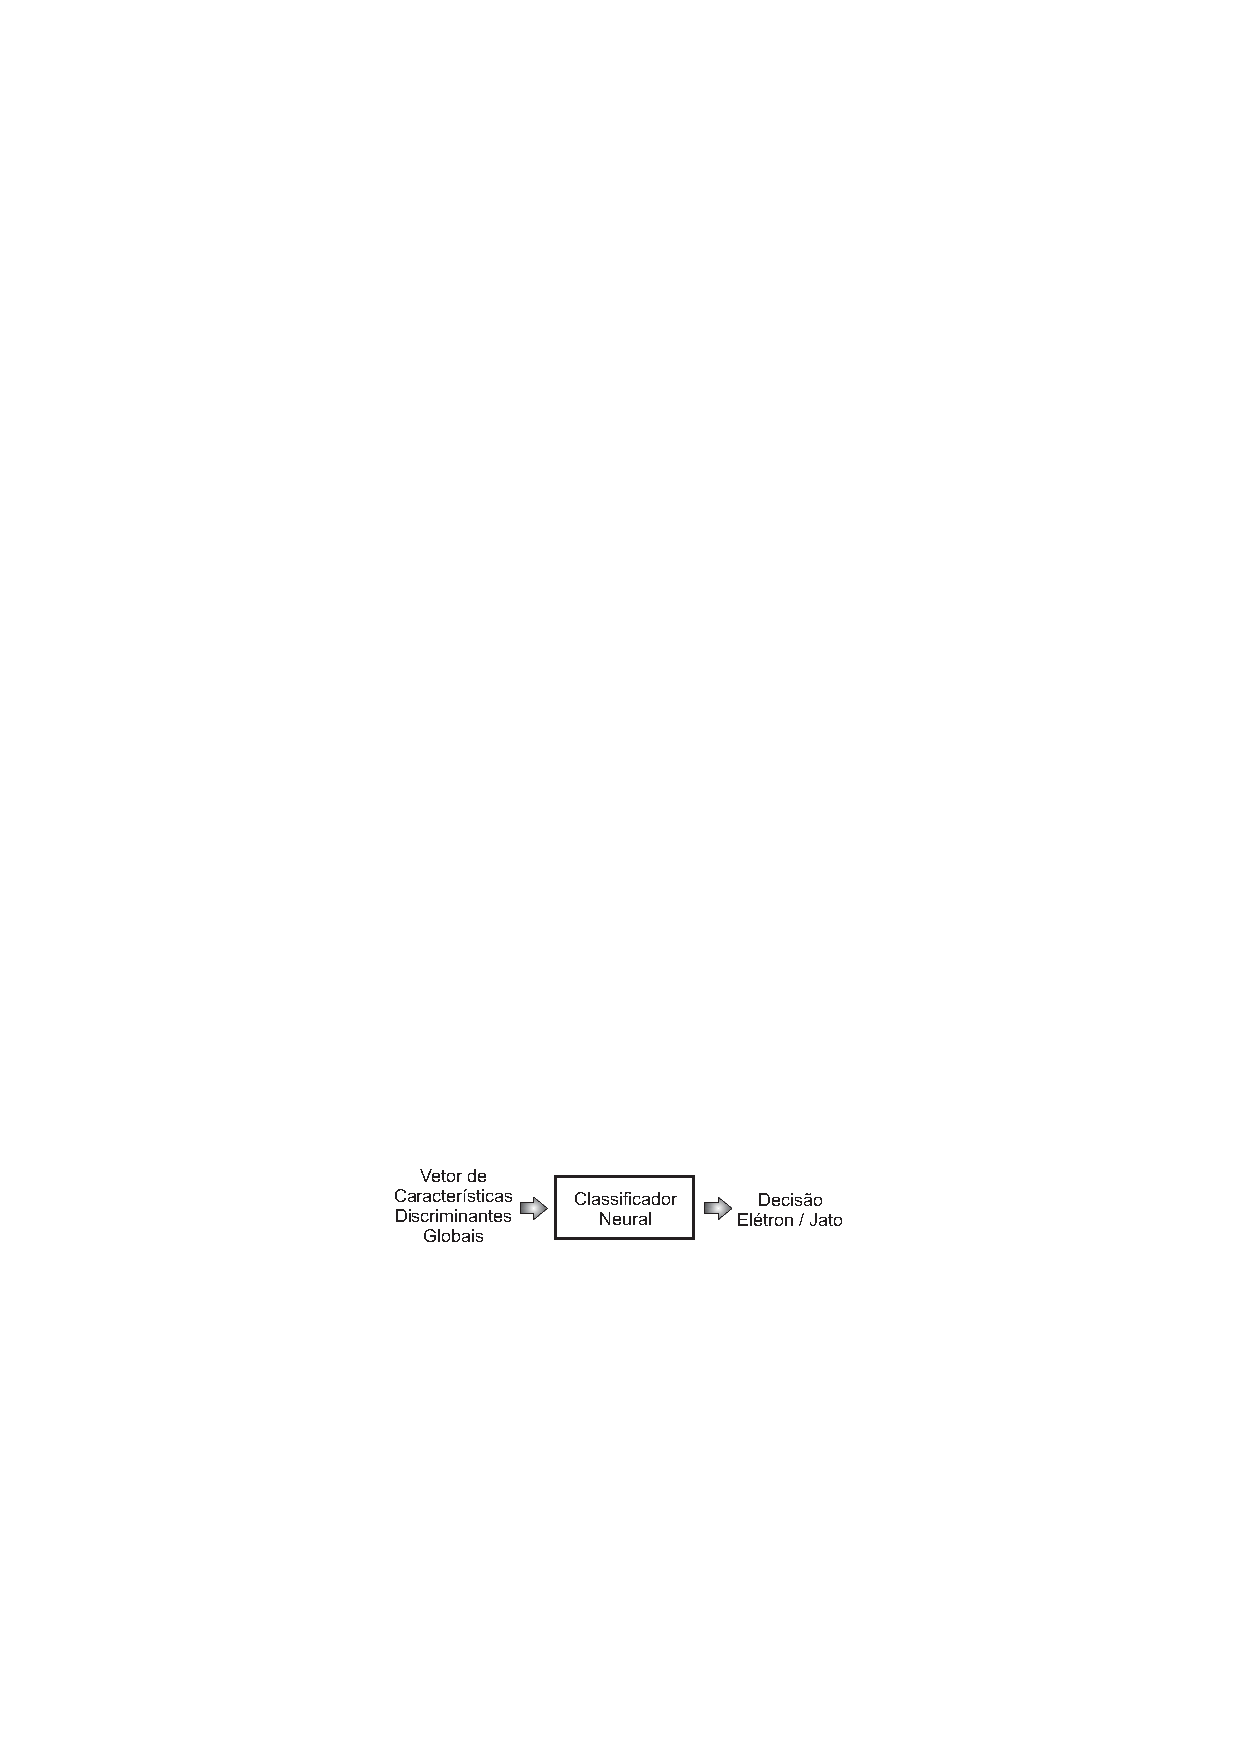
\includegraphics[width=0.5\textwidth]{imagens/classificacao_nao_segmentada.pdf}
}\\
\subfigure[]{%
    \label{fig:class_seg}
    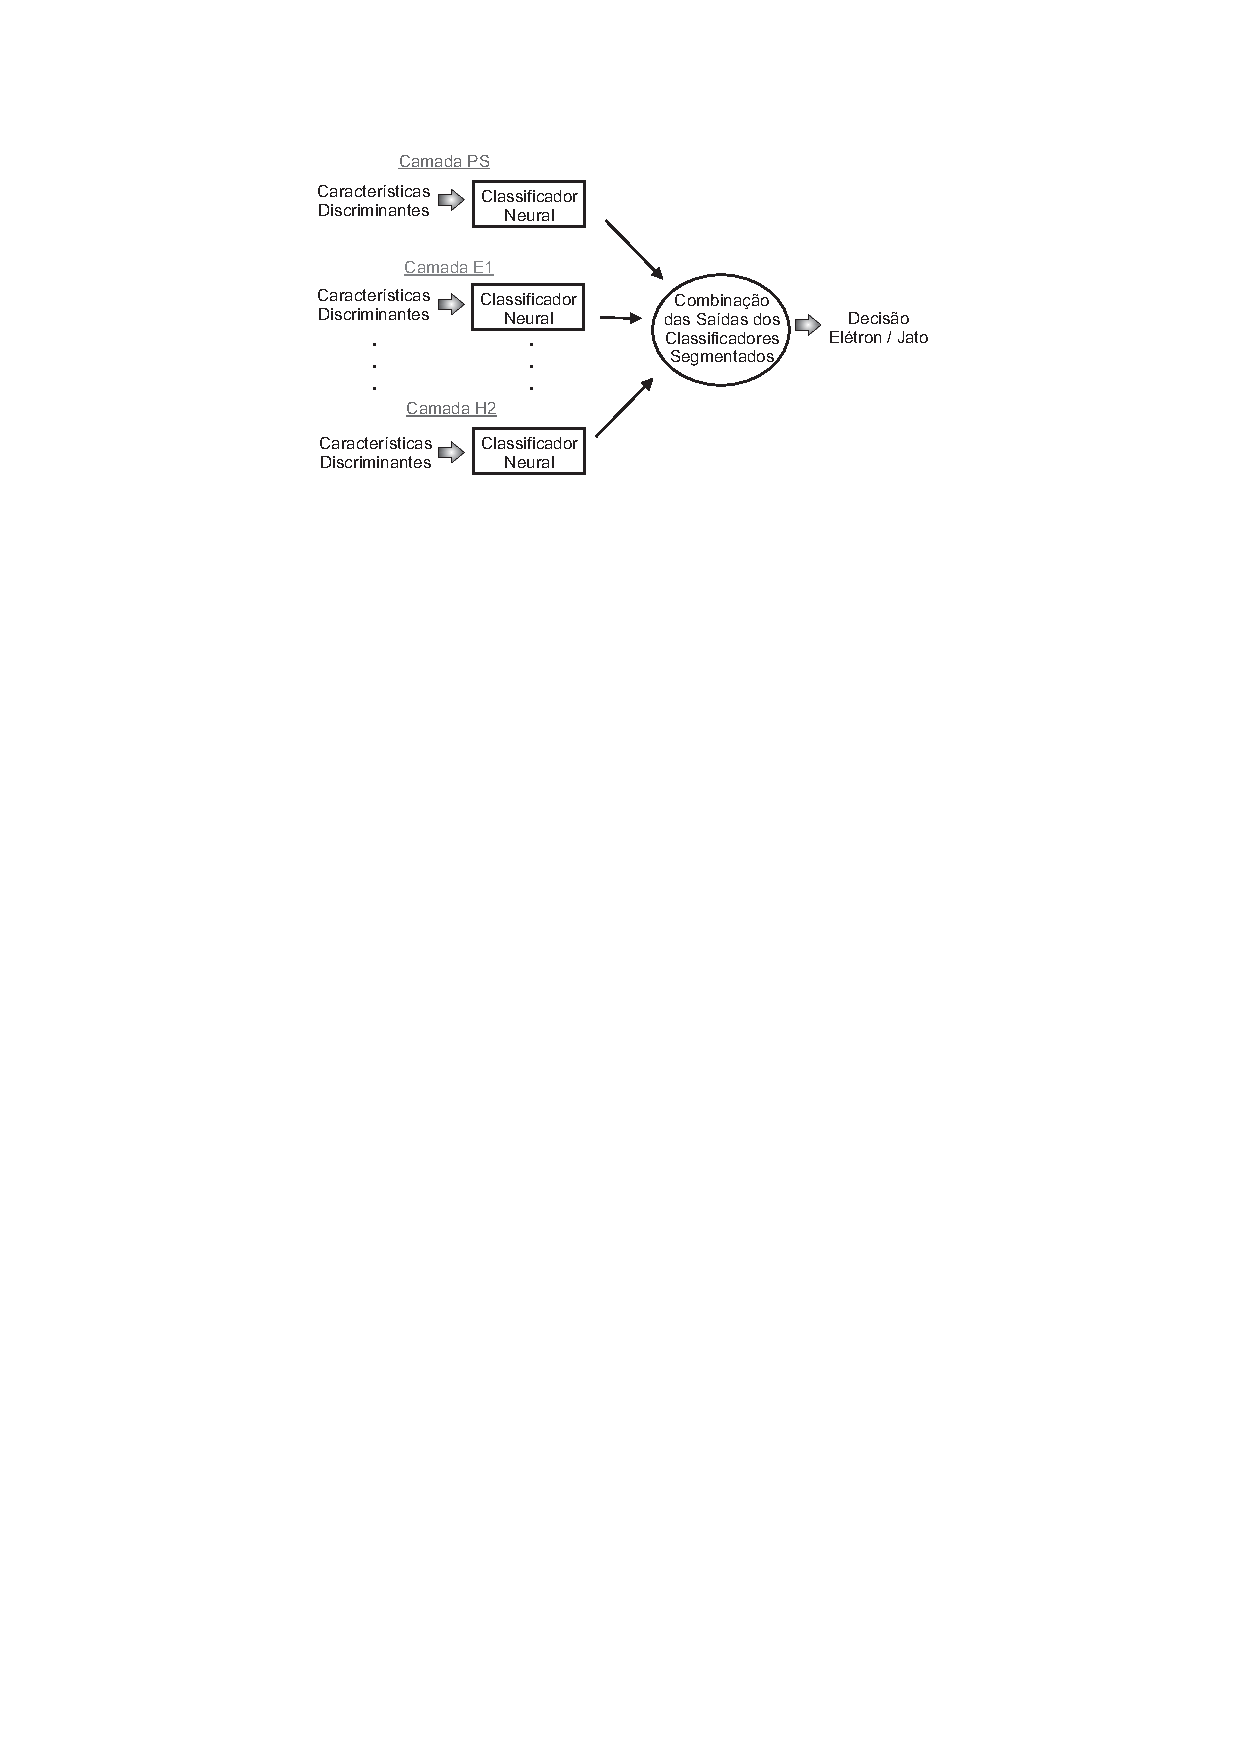
\includegraphics[width=0.7\textwidth]{imagens/classificacao_segmentada.pdf}
}
\caption[Abordagens de Discriminação: segmentada e não-segmentada.]
{Abordagem de discriminação não-segmentada
em~\ref{fig:class_nseg}, e segmentada em~\ref{fig:class_seg}. Extraído de 
\cite{tese_eduardo}.}
\end{figure}

\newacronym[type=Abrev]{rprop}{RPROP}{\emph{Resilient Back-propagation}}
\newacronym[type=Abrev]{mlp}{MLP}{\emph{Perceptron} Multicamadas}
\newacronym[type=Abrev]{mse}{MSE}{Erro Quadrático Médio}

A topologia de uma \gls{rna} composta de uma rede \gls{mlp} alimentada em
cascata, ou \emph{feed-forward}, com uma camada escondida está esboçada na
Figura~\ref{fig:topologia_rna}. Estão simbolizados três neurônios de saída, para
o caso de separação em três classes, mas a rede utilizada tem apenas uma saída,
suficiente para realizar a discriminação em duas classes, as partículas \gls{em}
compondo o sinal: elétrons, pósitrons e fótons; e o ruído físico: os
hádrons dos jatos hadrônicos. Os alvos utilizados para as classes foi de +1 para o
conjunto de sinal, e -1 para o conjunto de ruído físico.
A camada de entrada recebe o vetor de dados, com os 100 anéis normalizados, enquanto o número de 
neurônios na camada escondida varia conforme a representação dos dados, 
sendo determinado através de um estudo de exaustão. Todos os neurônios utilizam
função de ativação tipo tangente hiperbólica.

\begin{figure}[ht!]
\label{fig:topologia_rna}
\centering
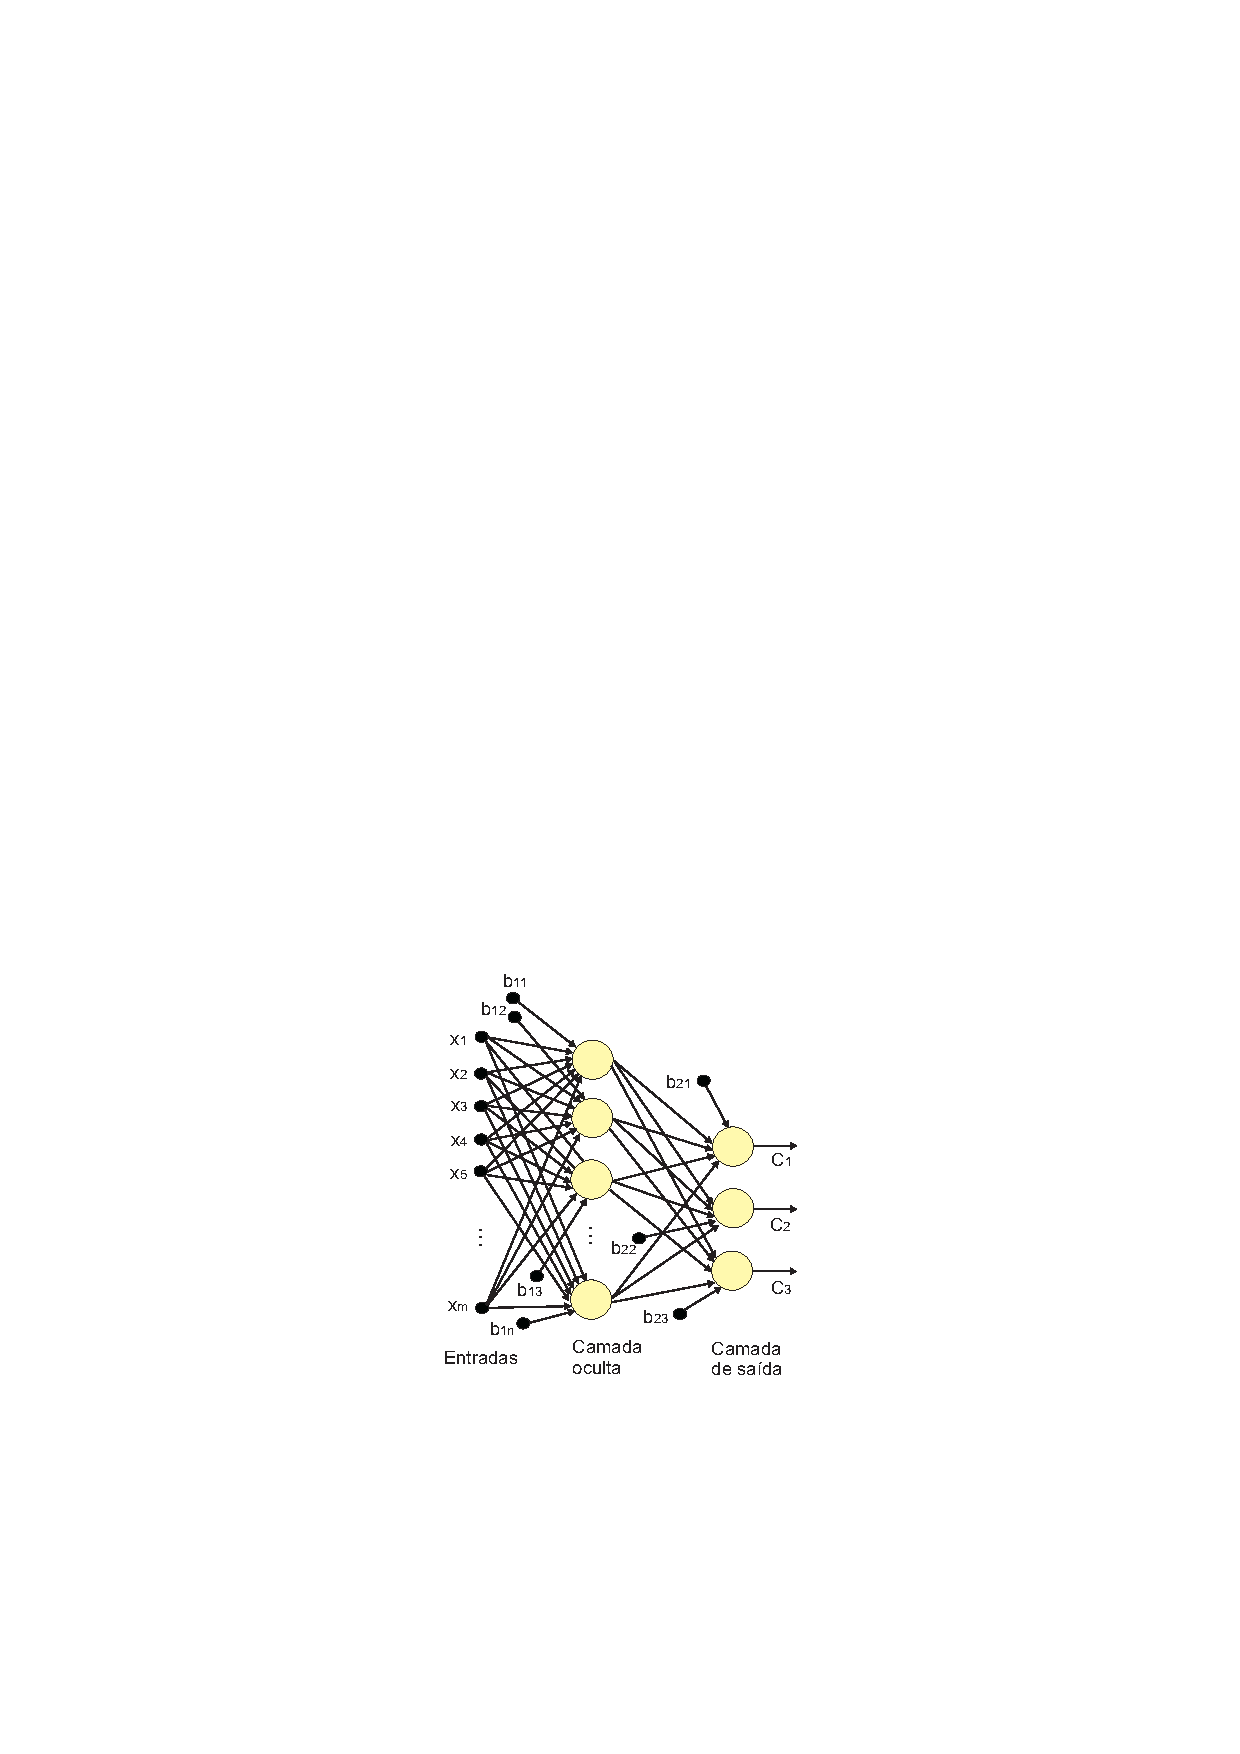
\includegraphics[width=0.4\textwidth]{imagens/topologia_rna.pdf}
\caption[Topologia de uma MLP alimentada em cascata.]{Topologia de uma
MLP alimentada em cascata. Extraído de \cite{tese_eduardo}.}
\end{figure}

É necessário realizar o treinamento das \glspl{rna} para que as mesmas possam, de
fato, reconhecer padrões. Para o processo de treinamento se
utilizou, na inicialização dos pesos, o algoritmo de \emph{Nguyen-Widrow} \cite{initnw}, 
enquanto no treinamento o \gls{rprop} \cite{rprop}, devido a sua simplicidade de uso e 
rápida convergência. Para realizar o treinamento secciona-se o conjunto de dados
em três partes: 

\newacronym[type=Abrev]{det}{\ensuremath{\text{DET}}}{Taxa de Detecção}
\newacronym[type=Abrev]{deteg}{\ensuremath{\text{DET}_{e/\gamma}}}{Taxa de Detecção de elétrons,
pósitrons e fótons}
\newacronym[type=Abrev]{detj}{\ensuremath{\text{DET}_{j}}}{Taxa de Detecção de hádrons}
\newacronym[type=Abrev]{fa}{\ensuremath{\text{FA}}}{Taxa de Falso Alarme}

\begin{enumerate} 
\item \textbf{Conjunto de treino} (neste estudo totalizando 50\% dos dados em
casos de pouca estatística e 33\% no oposto): 
no qual se será atualizado os pesos sinápticos da \gls{rna} de modo a minimizar uma função 
custo, na qual a utilizada foi o \gls{mse};
\item \textbf{Conjunto de validação} (16,6\%/33,3\%): utilizado para garantir a boa 
generalização da \gls{rna}; 
\item \textbf{Conjunto de teste} (33,3\% para ambos os casos): 
estatística não observada pela \gls{rna} durante seu treinamento, utilizada para 
testar sua perfomance. 
\end{enumerate}

Para a análise de eficiência de discriminação, alguns parâmetros precisam ser definidos:

\begin{enumerate}
\item \textbf{\gls{det}}: taxa de uma classe corretamente identificada pelo
discriminador. Geralmente se refere a taxa de sinal, no caso do Canal~\gls{eg} a
\gls{deteg}, mas também podendo ser utilizada para o caso de ruído, \gls{detj}.
Caso não identificado a classe de detecção, então se estará referindo a
\gls{deteg};
\item \textbf{\gls{fa}}: taxa da classe constituinte de ruído erroneamente
identificada pelo discriminador. No Canal~\gls{eg} a taxa de hadrôns que formam os
jatos hadrônicos identificados como \gls{eg}. Também pode
ser obtida como: $1-\gls{detj}$.
\end{enumerate}

\newacronym[type=Abrev]{sp}{SP}{Produto Soma-Produto}

Dois critérios podem ser utilizados para medir a figura de mérito da \gls{rna}
durante o treinamento, aplicando-se aos conjuntos de validação e teste: \gls{mse} 
e \gls{sp}. O \gls{mse} visa encontrar o ponto onde as saídas da \gls{rna} ficam
o mais próximo possível do alvo especificado. O \gls{sp} é relacionado por:

\begin{equation} \label{eq:produto_sp}
SP = \sqrt{ \sqrt{\gls{deteg}\times \gls{detj}}\times\frac{\gls{deteg}+\gls{detj}}{2}}\times100\%
\end{equation}

\noindent no caso de discriminação binária. Esse critério visa indicar ao
processo de treinamento o ponto onde a distinção máxima entre classes é obtido,
sendo o critério mais apropriado para \glspl{rna} destinadas ao reconhecimento de
padrões \cite{tese_torres}.

O número de épocas (ou iterações) de treinamento foi ilimitado, de forma que o
processo de treinamento somente é concluído quando ocorrem 50 falhas na tentativa
de melhora do critério utilizado como figura de mérito para a validação. 
Utilizou-se o critério \emph{Save the Best}, onde os pesos sinápticos na época com 
o melhor resultado da figura de mérito para o conjunto de teste são armazenados 
para a utilização da rede. Foi utilizado o critério de batelada, onde se sorteia os
dados a se realizarem o treinamento, com o tamanho do menor 
conjunto de dados de treinamento, geralmente sendo esse o de elétrons, para
evitar uma maior estatística de um dos conjuntos durante o treinamento. O
processo de treinamento é repetido $N$ vezes para evitar-se flutuação
estatística, inicializando novos pesos aleatórios para cada configuração 
testada.

\newacronym[type=Abrev]{roc}{ROC}{Região de Critério}

Após o treinamento é possivel especificar a \gls{det} (no caso de partículas \gls{eg}) 
e \gls{fa} através da escolha do limiar de decisão, aonde valores maiores ao limiar serão considerados
como \gls{eg} e os menores jatos. A escolha do limiar tem o seu compromisso
representados nas curvas \gls{roc}: quanto maior a \gls{det}, também será a
\gls{fa}. O \gls{sp} tenta conciliar o compromisso entre a detecção de
partículas \gls{eg} e jatos, o que não é desejado quando no \gls{sf}, onde se
deseja apenas filtrar os eventos a capacidade de armazenamento e processamento a
posteriori, evitando a perda prematura dos dados. Assim, o \gls{sp} é utilizado
apenas como figura de mérito para o treinamento das redes, e não como critério
de seleção para o limiar de decisão, que visa buscar a melhor \gls{det} sem
comprometer a capacidade de armazenamento e processamento a posteriori.

\section{O Sistema de Reconstrução (SR)}
\label{sec:sr}

O papel da reconstrução de física \cite{physics_perf_expected,atlas_computing_tdr}, 
realizada pelo \gls{sr}, é de derivar dos dados armazenados os parâmetros das partículas 
e auxiliar na informação necessária para a análise de física. 
Cada subdetector do \gls{atlas} utiliza um método individual de calibração de
sua informação, por exemplo, os calorímetros realizam a calibração da energias no
nível das suas células, e a informação armazenada pelos especialistas do
calorímetro para uma dada temporada é utilizada para evitar as células ruidosas ou mortas. 
Posteriormente cada canal de física utiliza a informação contida nos
subdetectores de modo a identificar as partículas de interesse e seus
parâmetros, realizando outras calibrações para garantir a melhor precisão
possível nesses parâmetros, de forma a facilitar e melhorar a qualidade de
descobertas, como a do bóssom de Higgs, entendimento de física ainda não bem
conhecida, como o quark \emph{top}, e outros objetivos citados em
\ref{ssec:obj_lhc}.

Muitas semelhanças podem ser observadas nos algoritmos do \gls{hlt}, em especial o
\gls{ef}, com o \gls{sr}. Na verdade, os algoritmos do \gls{sf} foram feitos
baseados no \gls{sr} com o objetivo de evitar ao máximo a polarização dos dados
armazenados. As diferenças entre os dois ambientes, como já foi dito, está na
maior restrição de tempo e robustez dos algoritmos no ambiente do \gls{sf}, de
forma que os algoritmos no \gls{sf} realizam análises menos refinadas. Por esse
motivo, os cortes utilizados no \gls{sf} são relaxados quando em comparação com
os do \gls{sr} para evitar a perda prematura de física de partículas em que não
se há muita certeza do que ocorreu. Nesses casos, prefere-se armazenar os
dados para o \gls{sf} analisar os eventos com mais detalhes e tomar uma decisão
com maior precisão, desde que isso não ultrapasse os recursos computacionais para 
armazenamento e processamento dos dados.

\subsection{\texorpdfstring{Algoritmo $e/\gamma$ Padrão}{Algoritmo eGamma Padrão}}
\label{ssec:egamma}

O algoritmo padrão de reconstrução de física a posteriori não é muito distinto
daquele descrito para o \gls{ef} da cadeia \gls{eg} no Tópico~\ref{ssec:cadeia_egamma},
inclusive já sendo realizadas algumas distinções entre os algoritmos que serão
aqui complementadas.

Primeiro, precisa-se ter em mente que o algoritmo a posteriori utiliza
parâmetros com maiores precisões. Calibrações, como a posição de \gls{eta}, e 
da energia depositada em cada camada é realizada com maior precisão. Outras
calibrações, como a posição em \gls{phi} e calibrações no nível de células,
também são realizadas no \gls{sr}, o que não ocorre para o \gls{hlt}.

Para a construção dos aglomerados de células no calorímetro se utiliza um algoritmo 
de janela deslizante \cite{sliding_window}.
Dois tipos de aglomerados podem ser construídos: os aglomerados \gls{em}, no caso de elétrons e fótons; 
e os combinados, na busca de jatos e identificação de
táons-léptons. São utilizados três passos no algoritmo, a construção das torres de
células, a procura por uma semente e o preenchimento do aglomerado, onde esses dois
últimos passos ocorrem juntos para os aglomerados combinados. 

Serão abordados apenas os aglomerados \gls{em}, uma vez apenas eles são
utilizados pelo Canal~\gls{eg}. O processo de construção é realizado apenas para 
$|\gls{eta}|<2,5$, onde é realizado a construção das torres, o Sistema de Calorímetria é 
dividido em uma grade de $0,025\times0,025$, através da soma da energia das
células das camadas longitudinais do \gls{ecal} contidas dentro da
região. Em seguida, uma janela de $5\times5$ torres
procura por uma região que ultrapasse um limiar para $\gls{Et} > 2,5$ GeV e 
que seja um máximo local (a idéia de máximo local é a mesma que àquela citada
para o \gls{l1}, presente no tópico já referênciado). Quando encontrado, é gerada uma
semente cuja posição é calculada através da ponderação de energia das células contidas 
em uma janela concêntrica a anterior mas menor ($3\times3$ torres) para evitar o
acumulo de ruído, com as posições das células.
Para remover duplicatas, ao se ocorrer multiplas sementes dentro de uma região
$2\times2$ torres, apenas a semente mais energética será armazenada. Os
aglomerados são reconstruídos com seus tamanhos 
específicos dependente da partícula e sua incidência ($3\times7$ para elétrons e fótons convertidos,
$3\times5$ para fótons não-convertidos quando incidindo no barril, e $5\times5$ na
tampa). O processo se inicia na \gls{e2} através da construção do
aglomerado a partir da posição da semente. Então o baricentro de energia é
calculado e propagado para a \gls{e1} e \gls{e3}, aonde são gerados os
aglomerados para essas camadas. Para o \gls{ps} é utilizado como centro o
baricentro de energia da \gls{e1}. A partir desse aglomerado serão retiradas 
as variáveis físicas utilizadas para representar a propagação do chuveiro, que
serão utilizadas para realizar a discriminação. Essas variáveis são algumas
daquelas contidas na Tabela~\ref{tab:cortes_em}.  
Um algoritmo alternativo também pode ser utilizado para a construção
de aglomerados topológicos, onde a idéia básica é agrupar as células 
vizinhas a semente que tiverem energia significante quando comparado ao ruído
esperado.

A informação do aglomerado é combinado com a reconstrução do traço
\cite{physics_perf_expected} das partículas para fazer a separação de elétrons e fótons, assim como melhorar o
potêncial de identificação de elétrons. O traço com o último ponto no \gls{trt}
com menor $\Delta\text{R}$ ao baricentro da \gls{e1} 
é utilizado para a combinação entre o traço e aglomerado. Os parâmetros do traço
e relação traço-aglomerado podem ser utilizados para gerar as outras variáveis
da Tabela~\ref{tab:cortes_em}.

Os requerimentos citados no \gls{sf} também se aplicam, sendo eles: \emph{loose}, 
\emph{medium} e \emph{tight}. Eles são utilizados para
identificar a característica da estatística utilizada para a análise.

Além do algoritmo padrão, a colaboração também realizou estudos de técnicas
multivariáveis, incluindo discriminadores de Máxima Verossimilhança, árvores 
de decisões ampliadas e redes neurais \cite{physics_perf_expected}.


\subsection{\texorpdfstring{$e/\gamma$ \emph{Calorimeter Ringer}
(EgCaloRinger)}{eGamma Calorimeter Ringer (EgCaloRinger)}}
\label{ssec:egringer}

Uma dificuldade encontrada para a introdução do \gls{hltringer} na cadeia de
filtragem \gls{eg} é sua configuração diferente ao \gls{t2calo}, causando o
receio, por parte da Colaboração, que ocorra a polarização dos dados. Por isso, foi requisitado a
implementação de uma versão do algoritmo para a análise a posteriori, permitindo
a utilização da ferramenta pela Colaboração e a confiança de que as partículas
selecionadas estão coerentes com a física. O \gls{egcaloringer} é a
implementação do algoritmo proposto para o ambiente \gls{sf}.

Embora a estrutura do algoritmo seja a mesma que aquela explicada para o \gls{l2}, no
Tópico~\ref{ssec:hlt_ringer}, realizando a construção dos anéis, normalizando e
então propagando para uma \gls{rna}, há diferenças nas versões devido aos ambientes de implementação, 
de maneira que as duas versões não são identicas. Primeiro, o \gls{sf} realiza a calibração da energia 
no nível das células, de forma que os anéis do \gls{egcaloringer} terão 
valores mais refinados de energia, enquanto o \gls{hltringer} utiliza o
valor cru medido pelo calorímetro. Outra mudança importante quanto a construção
dos anéis está na disponibilidade de todas as células para este, de forma que
os anéis serão completamente construídos, enquanto naquele apenas as
células disponíveis na \gls{roi} podem ser acessadas, deixando anéis em aberto. 
Finalmente, a diferença da semente utilizada para a construção dos anéis entre o \gls{sf} e \gls{l2}
também modificarão o processo de anelamento, onde o \gls{hltringer} utiliza
a célula quente da \gls{e2} contida na \gls{roi}, e sua versão a
posteriori o centro do aglomerado calculado pelo \gls{sf}, que contém uma ponderação da
distribuição de energia entre as células de todas as camadas do \gls{ecal}
contidas em uma região $3\times3$ torres (cada torre tem $0,025\times0,025$ em
$\gls{eta}\times\gls{phi}$), sendo uma posição muito mais realistica 
do centro do chuveiro.


\subsubsection{Implementação}
\label{sssec:egringer_impl}

A implementação do \gls{egcaloringer} foi realizada garantindo que a operação
dos algoritmos já implementados pela Colaboração não fossem afetados, alterando
o mínimo de código necessário dos destes e garantindo a operação normal da
reconstrução do Canal~\gls{eg}. O \gls{egcaloringer} não deveria ser executado
exceto quando explicitamente exigido pelo usuário. 

Para cumprir com esse requisito se idealizou a 
estrutura disposta na Figura~\ref{fig:implementacao_ringer}, de forma que apenas
quando adicionado a configuração via \glsdesc{jo} o algoritmo é executado.
Durante a inicialização, o \emph{egammaBuilder} organiza os algoritmos no
nível de informação dos subdetectores, adicionando os algoritmos de reconstrução
de traços, vértices e aglomerados do calorímetro, e chama a configuração do
\emph{EMPIDBuilder} que irá adicionar os algoritmos para a geração das variáveis
físicas utilizadas para a discriminação. Quando exigido na \glsdesc{jo}, o
processo de contrução dos anéis realizado pelo algoritmo \emph{RingerCaloTool} 
é adicionado durante a inicialização ao \emph{egammaBuilder}, 
que irá requisitar ao \emph{EMPIDBuilder} a adição da
execução do algoritmo de discriminação do \gls{egcaloringer} pelo
\emph{egammaEPiRingerCaloTool}, onde será executada a normalização especificada 
na \glsdesc{jo} e a propagação das informações contidas nos anéis normalizados 
na \gls{rna} também especificada. 

\begin{figure}[ht!]
\label{fig:implementacao_ringer}
\centering
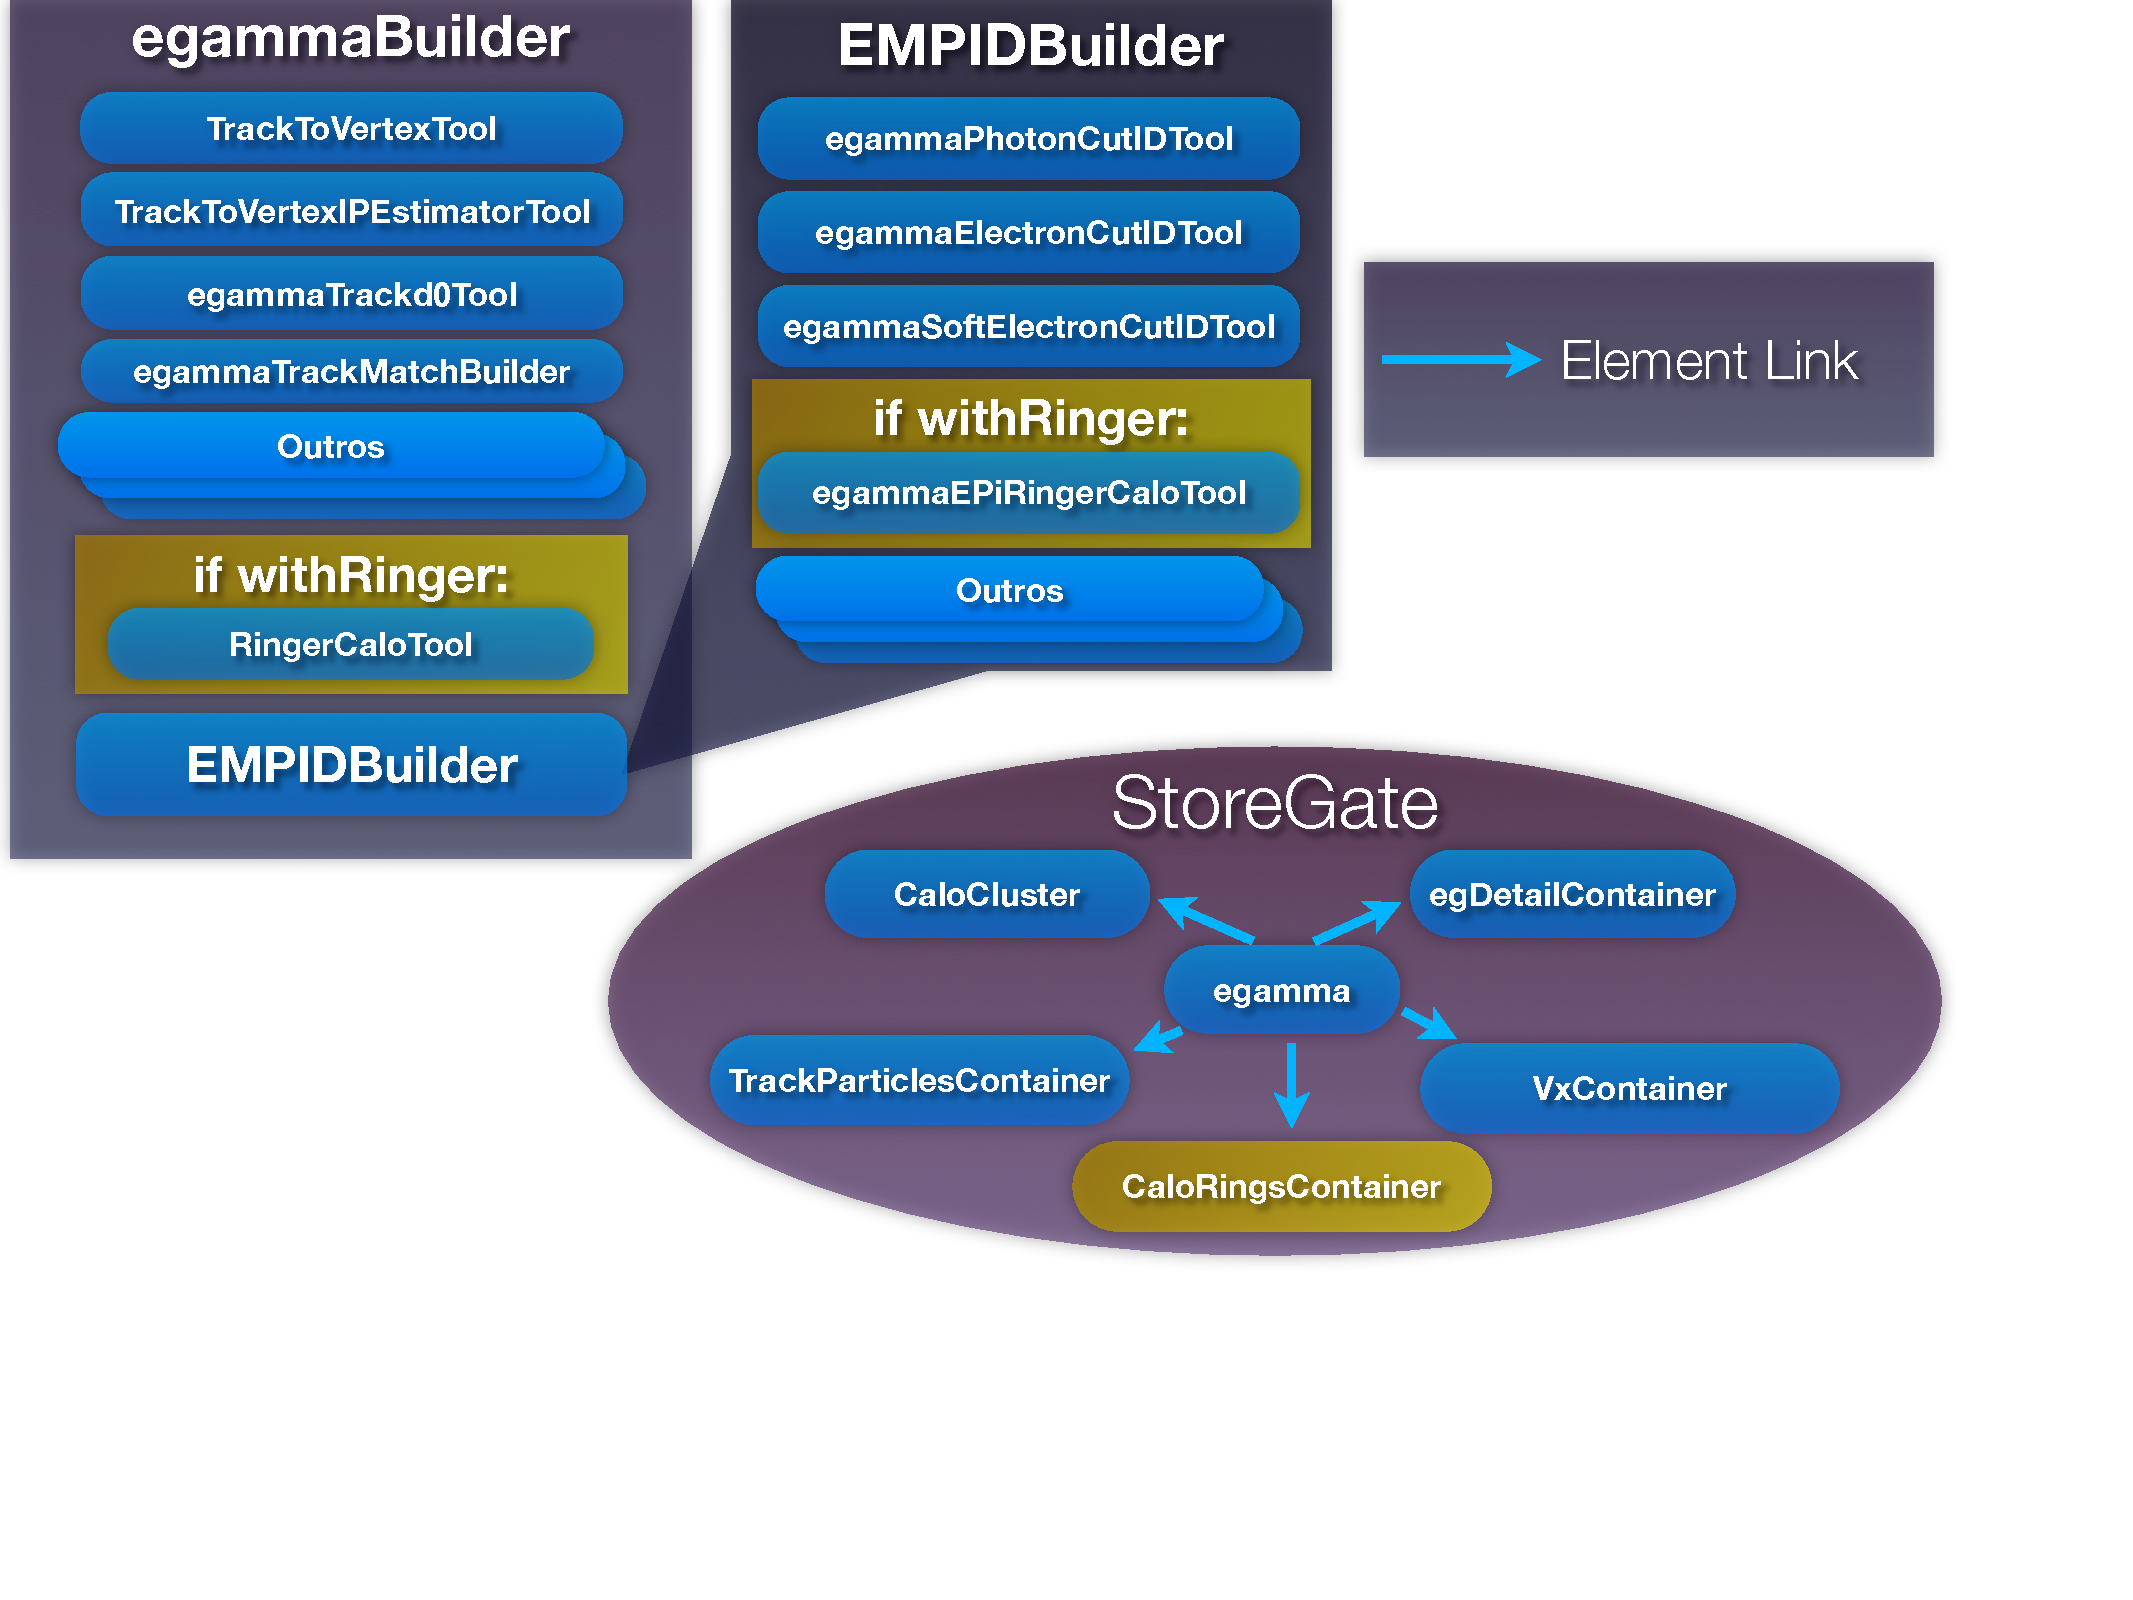
\includegraphics[width=1.0\textwidth]{imagens/implementacao_ringer.pdf}
\caption[Diagrama de implementação do \protect\gls{egcaloringer}]{Diagrama de
implementação do \gls{egcaloringer}.}
\end{figure}

Durante a execução, o \emph{egammaBuilder}
procura para cada evento os objetos de reconstrução dos subdetectores,
em busca por aglomerados e seus respectivos traços, criando um objeto 
\emph{egamma} transiente\footnote{Memória transiente é a informação contida na memória 
virtual do computador.} com as informações no \gls{sg}. A informação será
armazenada dentro recipiente \emph{egammaContainer} que irá ter \emph{Element
Links}\footnote{Pode ser interpretado com uma espécie de ponteiro de C++, embora
contenha outras informações além da posição de memória do objeto.} para o seu
respectivo aglomerado de células (\emph{CaloCluster}), traço
(\emph{TrackParticlesContainer}), vértice (\emph{VxContainer}), e detalhes como
propriedades do chuveiro, reconstrução do \emph{bremsstrahlung}, etc. (\emph{egDetailContainer}). 
O objeto \emph{egamma} é rotulado como um candidato a elétron, fóton, ou 
fóton convertido dependendo dessas informações. Se o \emph{RingerCaloTool}
estiver habilitado, durante a geração dos candidatos também será executado o
processo de geração dos anéis, que serão armazenados transientemente no
recipiente \emph{CaloRingsContainer}, também ligado ao seu objeto \emph{egamma}
aravés do elo gerado pelo \emph{Element Link}. Após o preenchimento do
\emph{egamma} com as informações do detector, o \emph{egammaBuilder} chama a
execução do algoritmo \emph{EMPIDBuilder}, onde serão geradas as variáveis 
físicas do algoritmo padrão, que serão armazenadas no \gls{sg} dentro do
\emph{egamma} através do objeto \emph{egPID}. Novamente se habilitado, após a
execução do algoritmo padrão, será realizada a execução do
\emph{egammaEPiRingerCaloTool}, que também irá armazenar a sua resposta no
\emph{egPID}.

As variáveis são então persificadas\footnote{Memória persistente é a informação
contida em disco rígido.}, onde os anéis e a saída neural só serão armazenados
se o \gls{egcaloringer} tiver sido habilitado. Na primeira implementação
realizada em Março de 2011, apenas a persificação no nível de \gls{aod} não foi
implementada. A análise em \glspl{esd} só pode ser realizada por \gls{ara},
sendo um processo relativamente complexo.
A compatibilidade com dados mais simples de análise foi realizada, como a
\gls{cbnta} e \emph{TrigEgammaNtuple}, um arquivo de análise especial gerado
pelo grupo \gls{hlt} do Canal~\gls{eg}. Essa versão está disponível apartir da
distribuição \emph{AtlasOffline-17-00-00} do \emph{Athena}.

Um segundo passo de implementação foi realizada em Agosto adicionando a
compatibilidade do algoritmo para \gls{d3pd} e \gls{aod}, mas ainda não foi
adicionado ao código oficial da Colaboração.



